\documentclass[sigconf,anonymous,review]{acmart}
%% \BibTeX command to typeset BibTeX logo in the docs
\AtBeginDocument{%
	\providecommand\BibTeX{{%
			Bib\TeX}}}

\setcopyright{none}
\copyrightyear{2025}
\acmYear{2025}
\acmDOI{XXXXXXX.XXXXXXX}

\acmConference[ACM CCS]{ACM Conference on Computer and Communications Security (ACM CCS)}{October 13--17,
	2025}{Taipei, Taiwan}
\acmISBN{978-1-4503-XXXX-X/18/06}

%%
%-------------------------------------------------------------------------------

\usepackage[linesnumbered,ruled,vlined]{algorithm2e}
\PassOptionsToPackage{table,xcdraw}{xcolor}
\usepackage{xcolor}

\usepackage{threeparttable}

\usepackage{graphicx} 
\usepackage[justification=centerlast]{caption}
\usepackage{subcaption} 

\usepackage{multirow}
\usepackage{array}


\usepackage[table,xcdraw]{xcolor} 
\usepackage{colortbl} 
\usepackage{booktabs} 
\usepackage{mdframed}
\usepackage{bm}

\usepackage{enumitem} 
\usepackage{hyperref}
\hypersetup{hypertex=true,
	colorlinks=true,
	linkcolor=blue,
	anchorcolor=blue,
	citecolor=blue}

% 防止孤行
\widowpenalty=10000
\clubpenalty=10000
\brokenpenalty=10000
\raggedbottom

\renewcommand{\topfraction}{0.95}
\renewcommand{\textfraction}{0.05}
\renewcommand{\floatpagefraction}{0.9}

\newcommand{\pandora}{{\scshape Pandora}\xspace}
%%%不需要下面这么复杂%%%
%\PassOptionsToPackage{colorlinks=true, linkcolor=blue, urlcolor=blue, citecolor=blue}{hyperref} % 传递选项
%\usepackage[colorlinks,
%linkcolor=blue,       %%修改此处为你想要的颜色
%anchorcolor=blue,  %%修改此处为你想要的颜色
%citecolor=blue,        %%修改此处为你想要的颜色,例如修改blue为red
%]{hyperref}

%%%%%%%%%%%%%%%%%%%%%%自定义四级标题%%%%%%%%%%%%%%%%%%%%%%
%\usepackage{titlesec}
%\titleclass{\subsubsubsection}{straight}[\subsubsection]
%\newcounter{subsubsubsection}[subsubsection]
%\renewcommand\thesubsubsubsection{\thesubsubsection.\arabic{subsubsubsection}}
%\titleformat{\subsubsubsection}[runin]{\normalfont\normalsize\bfseries}{\thesubsubsubsection}{1em}{}
%\titlespacing*{\subsubsubsection}{0pt}{1ex}{1ex}

\begin{document}
	
	%%标题修改%%%%
	%% The "title" command has an optional parameter,
	%% allowing the author to define a "short title" to be used in page headers.
	%\title{Evil Benign: Poisoning Attacks against Concept Drift Adaptation under Zero-Modification Condition for Target Malware}
	%\title{Devil Alliance: Poisoning Attacks against Concept Drift Adaptation under Zero-Modification Condition for Target Malware}
	%\title{Avoid arbitrarily expanding training dataset}
	%\title{Devil Alliance: Switchable Poisoning Attacks under multi attackers against Concept Drift Adaptation}
	% 2024-12-11-22-22-更新标题
	%\title{Devil Alliance: Switchable Poisoning Attack against Concept Drift Adaptation with Multi-Attacker Collaboration}
	% 2024-12-30-15-35-这个Switchable放到标题有点过了
	%\title{Devil Alliance: Poisoning Attack against Concept Drift Adaptation based on Active Learning with Multi-Attacker Collaboration}
	% 2025-3-15-20-01-去掉多攻击者
	%\title{Poisoning Attack against Concept Drift Adaptation based on Active Learning}
	% 2025-4-3-22-20-参考2025-CCF-B修改
	\title{Manipulating Uncertainty Ranking with Poisoning Attacks for Adversarial Concept Drift Adaptation}
	
	%%
	%% The "author" command and its associated commands are used to define
	%% the authors and their affiliations.
	%% Of note is the shared affiliation of the first two authors, and the
	%% "authornote" and "authornotemark" commands
	%% used to denote shared contribution to the research.
	%\author{Ben Trovato}
	%\authornote{Both authors contributed equally to this research.}
	%\email{trovato@corporation.com}
	%\orcid{1234-5678-9012}
	%\author{G.K.M. Tobin}
	%\authornotemark[1]
	%\email{webmaster@marysville-ohio.com}
	%\affiliation{%
		%  \institution{Institute for Clarity in Documentation}
		%  \city{Dublin}
		%  \state{Ohio}
		%  \country{USA}
		%}
	
	
	%%
	%% By default, the full list of authors will be used in the page
	%% headers. Often, this list is too long, and will overlap
	%% other information printed in the page headers. This command allows
	%% the author to define a more concise list
	%% of authors' names for this purpose.
	\renewcommand{\shortauthors}{Trovato et al.}
	
	%%
	%% The abstract is a short summary of the work to be presented in the
	%% article.
	\begin{abstract}
		
		Machine learning models have achieved remarkable success across various domains.
		Unfortunately, due to the continuously changing distribution of test data, deployed models can quickly become outdated—a phenomenon known as concept drift.
		To address this, Concept Drift Adaptation methods based on Active Learning (CDA-AL) have been proposed to enhance model performance by querying informative samples.
		However, limited research has been devoted to analyzing the robustness of CDA-AL.
		Our core insight centers on the susceptibility of CDA-AL's uncertainty-driven sample selection to adversarial manipulation. 
		The attacker crafts poisoned samples with high uncertainty to suppress the uncertainty ranking of the attack targets. 
		This manipulation misleads CDA-AL to misallocate its limited labeling budget to these less-informative poisoned samples, thus impeding the model's learning progress on the attack targets.
		
		PACDA's effectiveness is evaluated by using 7 experimental baselines, built by combining 7 models across 4 datasets.
		PACDA achieves an average attack success rate of over 90\% on three concept drift datasets with shorter time spans.
		Its effectiveness is further validated on a real-world concept drift dataset, APIGraph, which spans seven years and includes 300,000 samples.  
		On this dataset, PACDA attains an 88\% attack success rate while maintaining model stability, with F1-score fluctuations remaining within 0.2.  
%		In addition, we conduct long-term persistence evaluations and tests under constrained attacker capabilities, both of which yield attack success rates exceeding 80\%.
%		Our analysis of four existing countermeasuers show they fail to effectively counter PACDA, highlighting the need for robust solutions.
%		As a step forward, we propose an adaptive sample filtering method based on intra-cluster distance, which effectively mitigates PACDA attacks and enhances the performance of CDA-AL.
		
		
	\end{abstract}
	
	\begin{CCSXML}
		<ccs2012>
		<concept>
		<concept_id>10010147.10010178</concept_id>
		<concept_desc>Computing methodologies~Artificial intelligence</concept_desc>
		<concept_significance>300</concept_significance>
		</concept>
		<concept>
		<concept_id>10002978</concept_id>
		<concept_desc>Security and privacy</concept_desc>
		<concept_significance>500</concept_significance>
		</concept>
		</ccs2012>
	\end{CCSXML}
	
	\ccsdesc[500]{Security and privacy}
	\ccsdesc[300]{Computing methodologies~Artificial intelligence}
	
	
	\keywords{Concept Drift Adaptation, poisoning Attack, multi-Attacker, defenses}
	
	% 会显示在附录的最后
	%\received{20 February 2007}
	%\received[revised]{12 March 2009}
	%\received[accepted]{5 June 2009}
	
	\maketitle
	
	\section{Introduction}
\label{Sec: Introduction}
%Machine learning models are widely applied across various practical domains~\cite{2024-AAAI-AoA-estimation,2024-AAAI-Anomalous-User-Detection-on-Twitter,2024-AAAI-Designing-Biological-Sequences,2024-AAAI-Rumor-Detection}.
Supervised machine learning has been widely applied to critical security applications, including intrusion detection~\cite{yang2024recda} and malware analysis~\cite{fernando2024fesad}, where accurate and timely classification is essential for preventing breaches and mitigating threats.
However, as the gap between the testing and training data distributions widens over time~\cite{park2016active}, machine learning models performance on the testing data declines~\cite{malekghaini2023deep}.
This phenomenon, known as concept drift~\cite{2018-CCF-A-concept-drift-A-review,2024-1Q-An-overview-CDA,2024-1Q-survey-CDA}, is particularly dangerous because it can result in inaccurate predictions and potentially critical failures in high-stakes applications.

To address this challenge, numerous Concept Drift Adaptation (CDA) approaches have been proposed~\cite{2023-Q1-Concept-drift-handling,2023-Detecting-group-concept-drift-from-multiple-data-streams-1qu,aaaiYuLZ024}. 
Among them, Concept Drift Adaptation with Active Learning (CDA-AL)\cite{2023-Usenix-chenyizhen,liu2021comprehensive,krawczyk2018combining} has emerged as a promising strategy. 
In CDA-AL, the model selectively queries labels for the most informative data samples—typically those with the highest prediction uncertainty~\cite{ren2021survey,2023-Usenix-chenyizhen}—to detect and adapt to concept drift. 
These selected samples are manually labeled and incorporated into the training dataset for model retraining. 
As a result, CDA-AL improves the model's prediction accuracy on evolving data distributions.
%Obviously, providing ground-truth labels for high-uncertainty samples incurs a high cost, which is quantified as the labeling budget~\cite{yuan2022optical,hacohen2023select}.
%By learning from these informative yet uncertain samples, the model can adapt to the concept drift.
%The number of selected samples is referred to as the active learning labeling budget~\cite{hacohen2023select}, which represents the most costly human analysis resource in CDA-AL.

Existing research indicates that concept drift adaptation methods are vulnerable to data poisoning attacks.
This vulnerability arises because concept drift adaptation methods often incorporate selected samples from the test data into the training dataset.
Korycki et al.~\cite{2023-CCF-B-Adversarial-concept-drift-detection-under-poisoning-attacks} proposed a concept drift poisoning attack. In this attack, mislabeled concept drift samples are injected into the victim model’s training data to degrade its performance.
However, the threat model assumed in the above study differs from real-world concept drift adaptation, leading to three key limitations.
(1) Existing work assumes attackers can directly inject poisoned samples into the training set.
This contradicts CDA-AL, which adds only high-uncertainty samples to the training set.
(2) Prior work allows attackers to maliciously alter labels of poisoned samples~\cite{2022-ACM-Computing-Survey-Threats-to-training}. This is ineffective against active learning methods like CDA-AL. In CDA-AL, human annotators label new training data to ensure correctness.
(3) Poisoning attacks fall into two types: targeted and untargeted, based on their impact on the victim model’s performance.
Untargeted poisoning degrades the victim model’s overall performance. Targeted poisoning affects only the model’s predictions for specific attack targets.
Prior security research focuses on untargeted attacks.
In security-sensitive settings like malware detection, a drop in overall model performance raises alerts and reduces attack stealth.
The above limitations make existing concept drift poisoning attacks impractical in CDA-AL.

Because CDA-AL continuously collects testing data stream and selects retraining samples from it, the framework may become vulnerable to poisoning attacks. 
However, unlike traditional poisoning attacks that inject malicious samples directly into the training dataset in a batch manner~\cite{2022-ACM-Computing-Survey-Threats-to-training, 2024-SP-Offline-RL-Backdoor,2018-NIPS-Poison-frogs,2018-SP-poisoning-regression,2024-TIFS-Backdoor-Contrastive-Learning}, attacks against CDA-AL must exploit its adaptive learning process by planting poisoned samples in the testing data stream. 
This is a challenging task, as attackers must deceive the retraining process into mistakenly selecting poisoned samples for labeling, which are then incorporated into the retraining dataset—a scenario that, to the best of our knowledge, has not been explored before.

%The closest prior work is poisoning attacks or adversarial perturbations on CDA~\cite{, apruzzese2024adversarial};
%however, this area remains largely underexplored. 
%These studies typically assume that poisoned samples from the testing data stream are guaranteed to be incorporated into the retraining dataset, which does not align with the selective sample acquisition mechanism used in CDA-AL. 
%Moreover, their focus is primarily on untargeted attacks aimed at degrading overall model performance, overlooking the design of targeted poisoning strategies that can preserve stealth and global accuracy while manipulating specific predictions.
%However, CDA-AL operates on a continuously arriving testing stream, conventional poisoning methods~\cite{2024-SP-Offline-RL-Backdoor} \ziming{many more citations} that directly inject poisoned samples into the training set are no longer applicable. 
%Instead, the attacker must embed poisoned samples into the testing stream~\cite{2023-CCF-B-Adversarial-concept-drift-detection-under-poisoning-attacks}, allowing them to be indirectly included in retraining and thus degrade model performance.
%Nevertheless, existing poisoning attacks targeting concept drift typically assume that poisoned samples from the test stream are guaranteed to enter the training set, overlooking the selective sample acquisition mechanism employed by CDA-AL~\cite{2023-Usenix-chenyizhen}.
%Poisoning attacks on CDA-AL constitute a specialized yet critical research gap, as many security applications rely on manual analysis of complex samples to adapt to concept drift~\cite{2023-Usenix-chenyizhen}.
%Most existing poisoning attack studies focus on batch learning settings~\cite{2024-SP-Offline-RL-Backdoor,2024-SP-Audio-Backdoor}, where poisoned samples are injected into static training datasets to degrade model performance.
%In contrast, CDA-AL adapts to concept drift via streaming data, making streaming-based poisoning a more realistic threat~\cite{2021-Usenix-CDAE}.
%Furthermore, CDA-AL employs strict sample selection criteria~\cite{2023-Usenix-chenyizhen}, which significantly limits the inclusion of poisoned data and reduces the effectiveness of existing poisoning attacks.

In this paper, we present \pandora, a novel targeted \underline{p}oisoning \underline{a}ttack against co\underline{n}cept \underline{d}rift \underline{a}daptation with active learning via uncertainty \underline{r}anking m\underline{a}nipulation.
\pandora treats newly emerging concept drift samples in the testing stream as attack targets, aiming to prolong their misclassification while maintaining the overall performance of the victim model.
Specifically, \pandora generates high-uncertainty poisoned samples via adversarial perturbations.
These samples manipulate the uncertainty ranking in the testing data stream of each concept drift cycle, increasing their chances of being selected during active learning-based retraining.
The poisoned samples ultimately deplete the victim model’s limited labeling budget, thereby hindering effective learning on concept drift samples associated with the attack targets.
%that combines uncertainty-constrained search with problem space perturbations.
%Furthermore, we introduce a Shapley additive explanation method to attribute uncertainty to sample features.
%Based on features with high uncertainty influence, we optimize the generation of poisoned samples, expanding their uncertainty impact and further enhancing the robustness of the attack.
%Ultimately, \pandora prevents the victim model from acquiring informative knowledge about the attack target (e.g., attacker-specified malware samples) from the unlabeled testing data stream, leading to the misclassification of the attack targets.
%Regarding stealth, \pandora neither relies on label flipping nor degrades the victim model’s overall performance on previously collected data, thereby exhibiting strong stealthiness.
%Therefore, the attack remains undetected even if human experts within the CDA-AL framework analyze the poisoned samples.
%Moreover, our attack consumes a large portion of the labeling budget in CDA-AL, which represents the most expensive cost in active learning—human annotation.
%This cost is irreversible, as the human effort and time spent on poisoned samples cannot be recovered.
%Even if the attack is detected at a later stage, the damage caused by the depletion of these resources remains permanent.

%The key challenge of the \pandora is to generate high-uncertainty poisoned samples that are likely to be selected by the victim model, thereby exhausting its labeling budget.
%To address this, we first estimate the labeling budget consumption required to target a specific attack target.
%Then, we employ a constrained search strategy to identify high-uncertainty concept drift samples from the testing data as poisoning seeds.
%Based on these seeds, we propose a poisoned sample generation strategy that utilizes problem and feature space perturbations to exhaust the victim model's labeling budget.
%To improve the efficiency of feature-space perturbation, we employ SHapley Additive exPlanations (SHAP) for uncertainty-based feature attribution, enabling more precise feature manipulation.
%As a result, the victim model is unable to acquire informative samples related to the attack target, leading to its continuous misclassification.

%We conduct a comprehensive evaluation to demonstrate that existing CDA-AL methods~\cite{2023-Usenix-chenyizhen} are vulnerable to adversarial concept drift induced by poisoning attacks.
We evaluated the effectiveness of \pandora on five concept drift datasets: APIGraph~\cite{2020-CCS-APIGraph} , Androzoo~\cite{2016-Androzoo} and BODMAS~\cite{2021-PE-malware-dataset} for malware detection, MNIST~\cite{2017-MINIST-dataset} for image recognition, and SPAM~\cite{2010-Spam-Emali-dataset} for spam filtering.
%\pandora injects poisoned samples into the testing data stream during each retraining phase of the CDA-AL model.
Even when the number of poisoned samples is limited to no more than 0.05 of the testing stream, \pandora effectively extends the misclassification duration for over 80\% of the attack targets by at least one concept drift cycle across four datasets.
%Moreover, we observe a positive correlation between the duration of misclassification and the cumulative number of \pandora’s attacks during CDA-AL retraining.
%Empirical results on the APIGraph dataset—which exhibits the longest time span among all four datasets—show that as the cumulative number of attacks increases, more than 86\% of the attack targets experience a corresponding extension in misclassification duration.
%\pandora consistently prolongs the misclassification duration of attack targets across all four datasets, achieving an average success rate of over 80\%.
%Among these, APIGraph, which features the longest time span and largest number of attack targets, is the primary dataset for our experimental validation.
%For instance, over a 72-month period, we conducted attacks on more than 1,000 individual targets and achieved an average success rate of 88\%.
To better understand the effectiveness of \pandora under different conditions, we further analyze key factors influencing attack effectiveness, including sample selection strategies of active learning, the victim model's labeling capacity, and methods for constructing sample features.
Notably, \pandora remains effective across all settings, and we provide an in-depth analysis of the relationship between influencing factors and attack performance.

We also evaluated the effectiveness of existing targeted poisoning defense techniques against \pandora, including data sanitization~\cite{chen2018detecting}, robust training~\cite{DFP}, and input-time detection~\cite{2023-ICCV-Trigger-Detect}.
This corresponds to the three stages of potential defense methods for CDA-AL: data processing, sample selection, and model retraining.
Experimental results indicate that these methods struggle to effectively distinguish between poisoned and clean samples, leading to the failure of defenses against \pandora.
These findings highlight the urgent need for new defense mechanisms against \pandora.
To address this, we propose a poisoned sample filtering approach based on intra-cluster distance to mitigate the effects of \pandora.
Under the same poisoning attack settings, our defense method successfully prevents the extension of misclassification duration for 40\% of the attack targets.
The contributions of this paper are as follows:
\begin{itemize}
	\item We present \pandora, the first targeted poisoning attack against CDA-AL.
	\pandora causes the misallocation of labeling budget to poisoned samples by manipulating the uncertainty ranking of testing data, leading to misclassification of attack targets during the adaptation process.
	
	\item We introduce a strategy for generating high-uncertainty poisoned samples.
	By applying problem-space adversarial perturbations and concept drift direction misguidance, our method generates enough poisoned samples to exhaust the limited labeling budget.
	
	\item We evaluate \pandora across diverse datasets, model architectures, and sample selection strategies, demonstrating its effectiveness in prolonging the misclassification duration of attack targets.
	To demonstrate our commitment to open-source, we have made an anonymized version of the code available at \href{https://anonymous.4open.science/r/\pandora-Attack-B730}{https://anonymous.4open.science/r/\pandora-Attack-B730} 
	
	\item We identify critical limitations in existing defense mechanisms against \pandora.
	We present a poisoned sample filtering method based on cluster-adaptive distance to mitigate this attack.
\end{itemize}


	
	%\section{Preliminaries}
%This section presents the process of CDA-AL, as well as representative data poisoning attacks developed for static (non-drift) learning environments.

\section{Background: Concept Drift Adaptation with Active Learning}
\label{Sec: Concept Drift Adaptation}

CDA-AL is a paradigm that enhances model performance by identifying high-uncertainty samples from the testing data~\cite{2023-Usenix-chenyizhen,park2016active,vzliobaite2013active}.
%\begin{figure}[t]
%	\centering
%	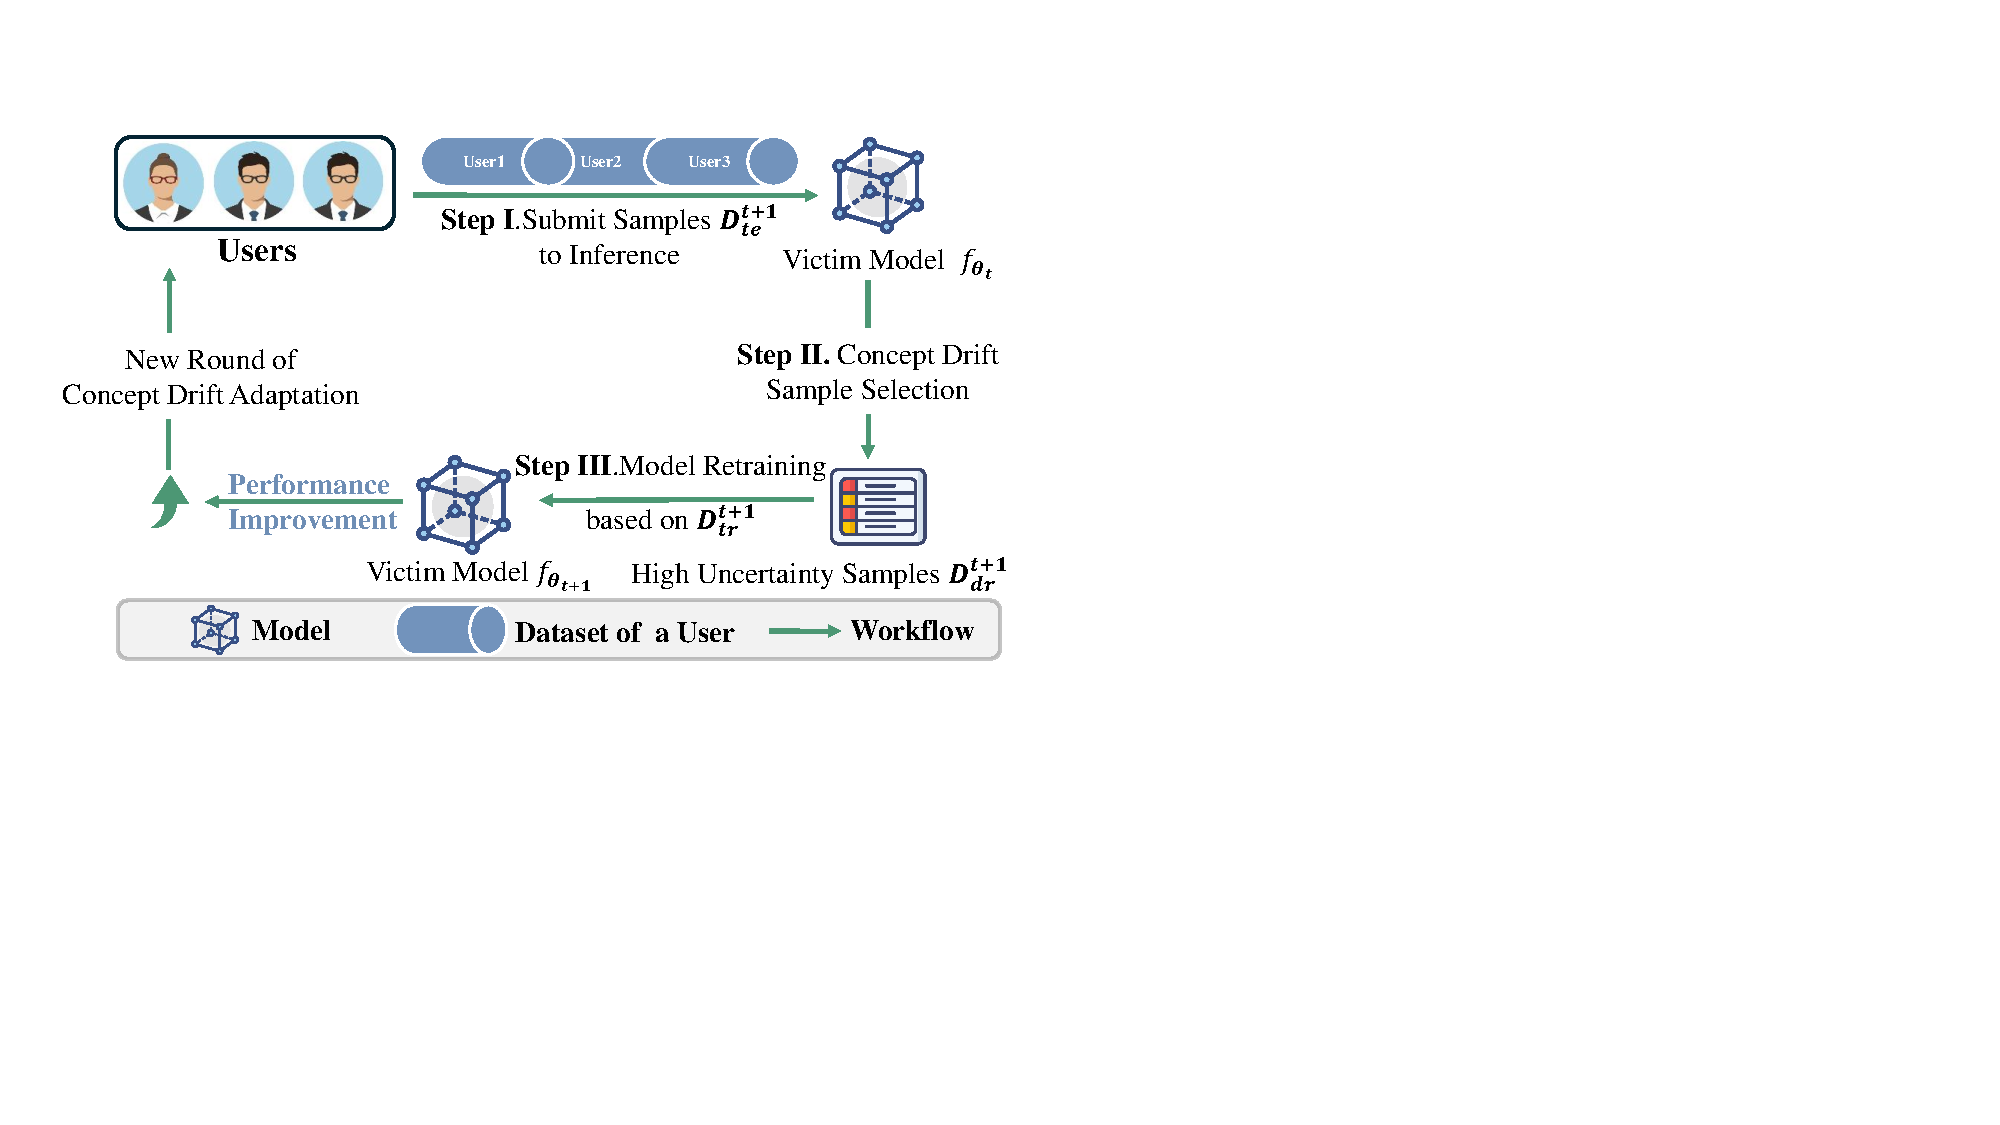
\includegraphics[width=\linewidth,keepaspectratio]{Graph/Intro_graph/Background/Concept_Drift_Adaptation_Based_Active_Learning_2025_3_27_15_23.pdf}
%	\caption{Concept drift adaptation based active learning}
%	\label{fig: CDA-AL-1}
%\end{figure}
%The overall process is illustrated in Figure~\ref{fig: CDA-AL-1}.
For consistency, we refer to the concept drift adaptation model as the victim model throughout this paper.
The entire concept drift process is composed of multiple concept drift cycles.
%The number of concept drift cycles is set to $n$ in our subsequent discussions.
Let $f_{\bm{\theta}_{n}}$ denote the victim model trained on the training data $\bm{D}^{n}_{tr}$ in concept drift cycle $n$.
$\bm{\theta}_{n}$ denotes the retrained model parameters at the end of concept drift cycle $n$, while $\bm{D}^{n}_{tr}$ refers to the updated training dataset used by the victim model during that cycle.
The unlabeled testing dataset $\bm{D}_{te}^{n}$ comprises all samples collected by the victim model throughout concept drift cycle $n$.
For concept drift cycle $n$, the concept drift adaptation process generally consists of three steps:

\emph{Step I}: Victim Model $f_{\bm{\theta}_{n-1}}$ performs inference on the input $\bm{\mathrm{x}}_{i} \in \bm{D}_{te}^{n}$ and obtain the classification confidence vector $\bm{\mathrm{c}}_{i} = f_{\bm{\theta}_{n-1}} \left( \bm{\mathrm{x}}_{i} \right)$.
	The different dimensions of $\bm{\mathrm{c}}_{i}$ indicate the model's confidence that the input $\bm{\mathrm{x}}_{i}$ belongs to a specific sample label. 
	The label with the highest confidence is selected as the predicted label $\overline{y}_{i}$ on the input $\bm{\mathrm{x}}_{i}$.

\emph{Step II}: %Based on the confidence vector $\bm{\mathrm{c}}_{i}$ obtained in the previous step, 
	The uncertainty score $\bm{\mathrm{u}}_{i}$ of $\bm{\mathrm{x}}_{i}$ is measured.
	For example, uncertainty can be measured as one minus the maximum softmax output of the network~\cite{2023-Usenix-chenyizhen}:
$\bm{\mathrm{u}}_{i} = 1-\max(\bm{\mathrm{c}}_{i},1-\bm{\mathrm{c}}_{i})$.
	We use $uncer()$ to denote uncertainty measures in the following discussion.
	
\emph{Step III}: High-uncertainty samples are selected from the testing data $\bm{D}_{te}^{n}$ as concept drift samples $\bm{D}_{dr}^{n}$.
	The size of $\bm{D}_{dr}^{n}$ is determined by the manual labeling capacity, referred to as the labeling budget $\beta$.
	Then, the concept drift data $\bm{D}_{dr}^{n}$ is manually labeled to get the ground truth label and added to the existing training data $\bm{D}^{n-1}_{tr}$ to form an updated training data $\bm{D}^{n}_{tr} = \bm{D}_{tr}^{n-1} \cup \bm{D}_{dr}^{n}$.
	The victim model $f_{\bm{\theta}_{n-1}}$ is then retrained on the updated training data $\bm{D}^{n}_{tr}$ to yield an updated model $f_{\bm{\theta}_{n}}$, as described in Equation~\ref{active learning loss}.
	\begin{equation}
		\begin{aligned}
			\bm{\theta}_{n} = \arg\min_{\bm{\theta}_{n-1}} \sum_{\bm{\mathrm{x}}_{i} \in \bm{D}^{n}_{tr}} \mathcal{L} \left( f_{\bm{\theta}_{n-1}}\left( \bm{\mathrm{x}}_{i}\right) , y_{i}  \right) \\
		\end{aligned}
		\label{active learning loss}
	\end{equation}


%\textbf{didn't you already mention this??? what is the point of this paragraph??}
%In this paper, we refer to the samples selected by the uncertainty-based selection strategy as concept drift samples, although they may not be directly affected by drift.
%Uncertainty can also result from other factors, such as when samples lie near the decision boundary in a stable distribution.
%Following prior work~\cite{2023-Usenix-chenyizhen}, we do not explicitly distinguish these samples in the following discussion since such differentiation pertains to concept drift detection rather than adaptation.

\begin{comment}
\subsection{Data Poisoning Attacks}
\label{Sec: Data Poisoning Attacks}

In data poisoning attacks, the attacker constructs poisoned data to degrade the performance of the victim model.
The most common strategy is to inject poisoned samples into the victim model’s training dataset.
As noted by Tian et al.~\cite{2022-ACM-Computing-Survey-Poisoning-attacks-and-countermeasures-in-ML} and Wang et al.~\cite{2022-ACM-Computing-Survey-Threats-to-training}, such attacks are generally categorized as targeted or untargeted.
Untargeted poisoning attacks aim to hinder the convergence of the victim model and eventually lead to denial-of-service~\cite{pmlr-v20-biggio11,2023-AAAI-yuuntargeted,wang2023analysis}.
The challenge with untargeted attacks is that they aim to degrade the performance across all data~\cite{2024-CCS-Phantom}.
Therefore, the effect of poisoned samples must outweigh that of the clean training data.
In contrast, targeted poisoning attacks aim to manipulate the victim model into making incorrect predictions on specific inputs~\cite{2024-TIFS-Backdoor-Contrastive-Learning,2021-Usenix-Poisoning-Attack-Explanation-guided-Backdoor,2023-SP-backdoor-attack}.
The inputs for which the model’s predictions are compromised are called attack targets. 
To launch a targeted poisoning attack, an adversary needs to
inject malicious knowledge into the training data while keeping other knowledge unaffected~\cite{2022-ACM-Computing-Survey-Poisoning-attacks-and-countermeasures-in-ML}.
\end{comment}

	
	\section{Threat Model}
\label{Sec: Threat Model}

The goal of \pandora is to ensure persistent misclassification of the attack targets by the victim model throughout the CDA-AL process, as shown in Equation~\ref{PANDORA-Formulation}.
\begin{equation}
	\begin{aligned}
			\max_{ \{ D_{poi}^{n} \}_{n=1}^{T} } \sum_{n=1}^{T} \mathbb{I}[ f_{\bm{\theta}_{n}}(x_{tar}) \neq y_{tar} ]
	\end{aligned}
	\label{PANDORA-Formulation}
\end{equation}
Let $x_{tar}$ denote the target sample with ground-truth label $y_{tar}$, and let $T$ represent the total number of drift periods.
We use $\mathbb{I}[\cdot]$ as an indicator function that equals $1$ if the condition holds and $0$ otherwise.
At each cycle $n$, the attacker injects poisoning data $D_{poi}^{n}$ into the training process, resulting in an updated victim model $f_{\theta_{n}}$ trained with $D_{poi}^{n}$.
By continuously introducing such poisoned data across cycles, the attacker aims to drive $f_{\theta}$ to misclassify the target sample $x_{tar}$.

We assume attackers cannot access the victim model's internal parameters or influence its training process~\cite{2017-ASIACCS-Black-Box-Attack}, including manual labeling of CDA-AL~\cite{2023-Usenix-chenyizhen}.
Attackers can only submit samples to the victim model for querying to obtain outputs such as sample uncertainty scores~\cite{2025-Baidu-Image-Recognition} and predicted labels~\cite{Virustotaluploadinterface}.
Additionally, attackers are presumed to have access to public data and the resources required to train surrogate models~\cite{2023-AAAI-surrogate-model-for-adversarial-attack}.
Consistent with previous research on active learning attacks~\cite{2021-Usenix-active-learning-backdoor}, we assume the attacker typically has knowledge of the victim model's labeling budget settings.
Moreover, the attacker can access the victim model’s prediction uncertainty.
This is based on the observation that existing machine learning services (e.g., image recognition~\cite{2025-Baidu-Image-Recognition}) provide uncertainty information to help users better interpret and utilize the prediction results.
In addition, it is important to note that although CDA-AL systems involve human analysts, their primary role is to provide reliable labels for concept drift samples~\cite{2023-Usenix-chenyizhen}.
As long as \pandora does not rely on malicious label manipulation, the attack remains inconspicuous to human analysts.
In PANDORA, all poisoned samples follow the threat model of clean-label poisoning attacks, where the labels of poisoned samples are never maliciously altered.
Compared with existing clean-label poisoning~\cite{2018-NIPS-Poison-frogs} threat models that assume free insertion of poisoned samples into the training dataset and require access to the victim model’s parameters, PANDORA imposes stricter constraints: poisoned samples must exhibit high uncertainty, and no parameter access is needed.
Therefore, PANDORA operates under a more stringent threat model than prior clean-label poisoning attacks.
	
	%\section{Design Rationale}
%\subsection{Design Challenges}
%
%\pandora faces three key challenges.
%(1) The sample selection strategy deployed in CDA-AL restricts the arbitrary injection of poisoned samples into the training data.
%Therefore, attackers must ensure that the victim model selects poisoned samples for labeling.
%(2) The sample labeling process in active learning is based on manual analysis, meaning the labels of all poisoned samples in the training data must remain correct.
%The attacker cannot degrade the victim model’s concept drift adaptation performance by tampering with the sample labels~\cite{2018-NIPS-Poison-frogs,2019-NIPS-Transferable-clean-label-poisoning-attacks-on-deep-neural-nets}.
%(3) Existing targeted poisoning attacks are typically evaluated for effectiveness on models with fixed parameters. 
%For example, backdoor attacks are often evaluated on pre-trained models~\cite{2024-TIFS-Backdoor-Contrastive-Learning,2021-Usenix-Poisoning-Attack-Explanation-guided-Backdoor,2023-SP-backdoor-attack}.
%In contrast, \pandora must ensure its attack remains effective as the victim model continuously updates its parameters.
%\pandora tackles the first two challenges.
%The final challenge is addressed through continuous attacks on the concept drift adaptation process.
%Additionally, we validate the persistence of the attack’s effectiveness on concept drift data spanning seven years, as discussed in Section~\ref{Sec: Single Attack Targets}.


\begin{figure}[t]
	\centering
	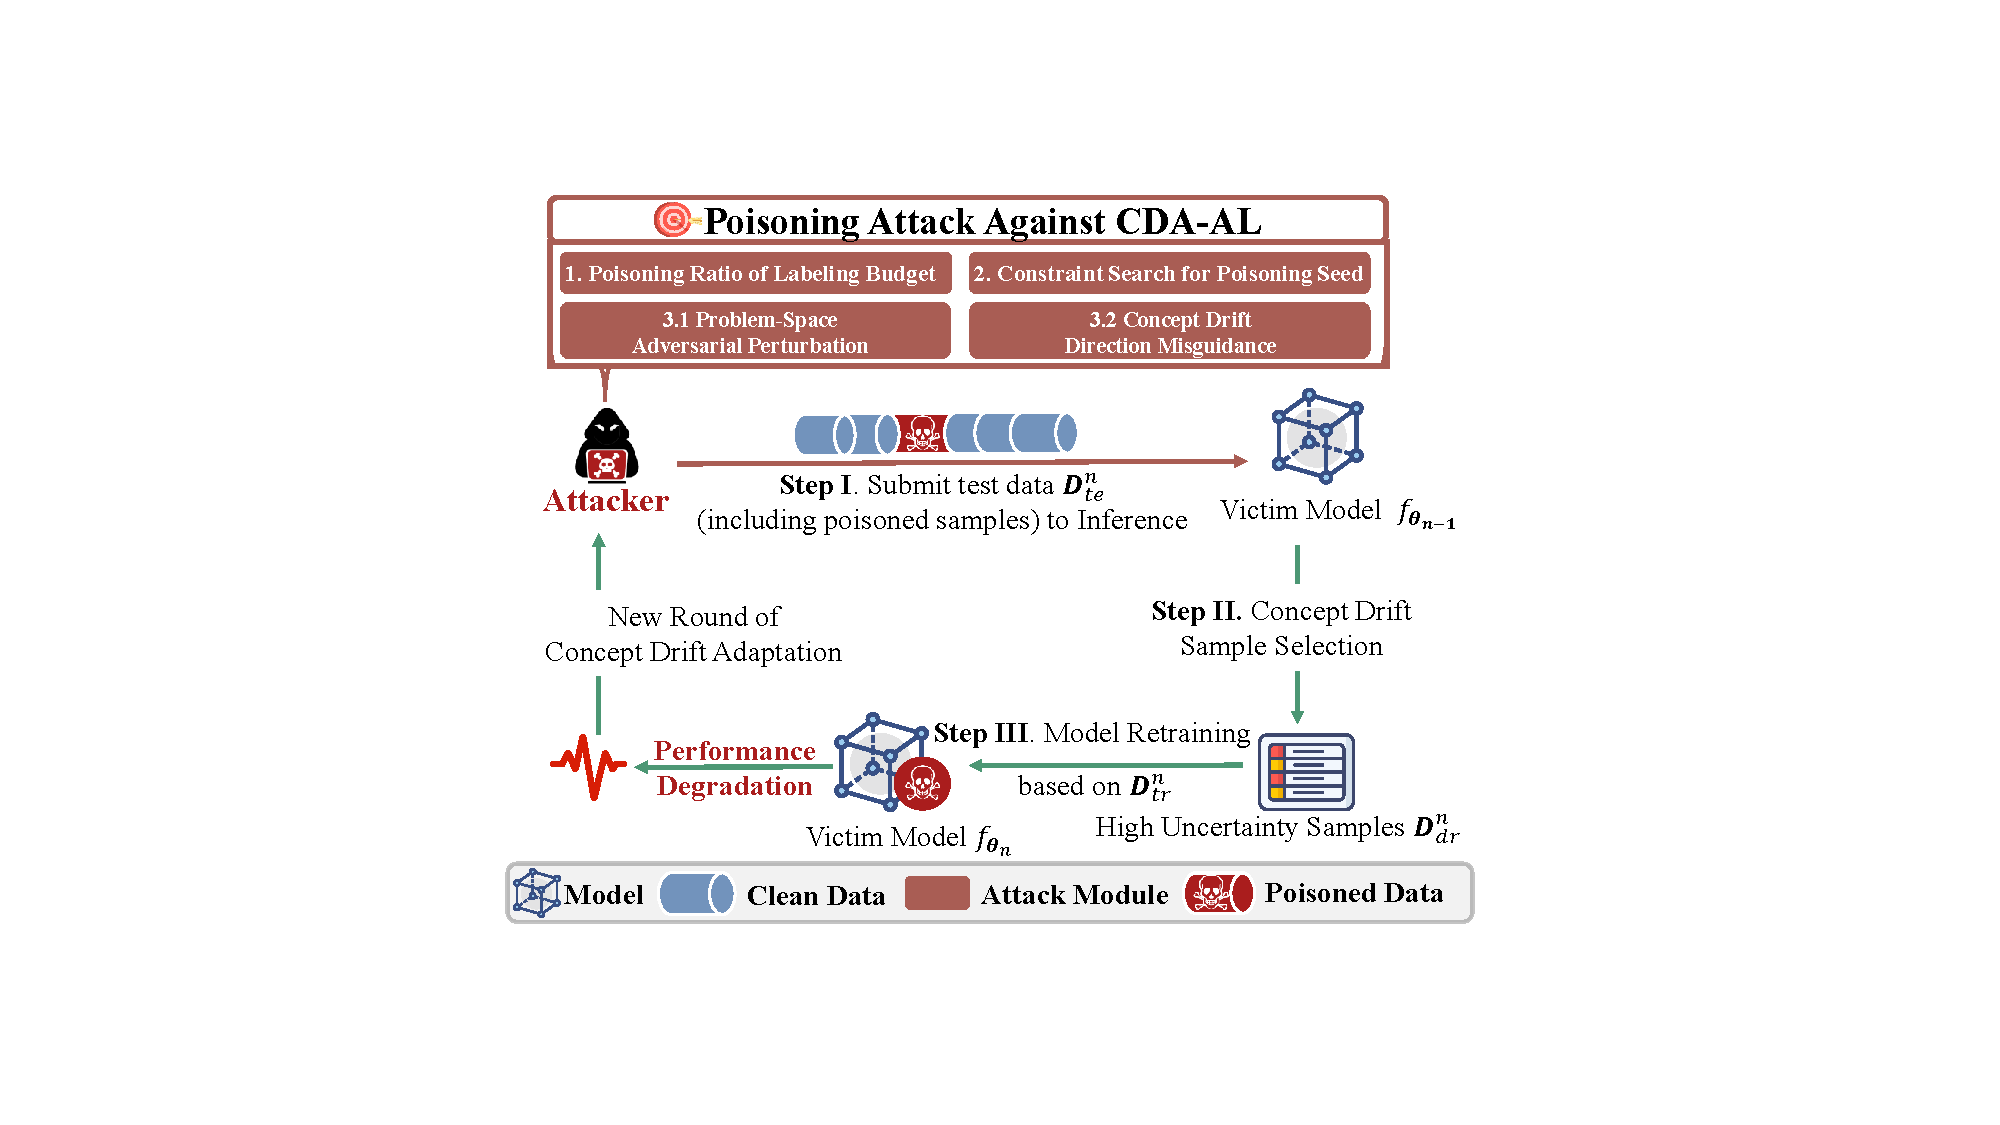
\includegraphics[width=\linewidth,keepaspectratio]{Graph/Attack_Method/PACDA_attack_process_2025_6_6_01_07.pdf}
	\caption{Poisoning Attack against CDA-AL}
	\label{fig:Attack Process}
\end{figure}

\section{\pandora}
\label{Sec: Attack Method}

We present the \pandora framework, illustrated in Figure~\ref{fig:Attack Process}.
The process begins by estimating the required poisoning ratio of the labeling budget based on the specified attack targets.
By injecting poisoned samples into the testing data stream, the attacker determines which knowledge the victim model can or cannot acquire.
Subsequently, we search the testing data stream to identify potential poisoning seeds.
Based on the identified poisoning seeds, \pandora generates poisoned samples through adversarial perturbations in the problem space, further enhancing the attack effectiveness by misleading the direction of concept drift.
Ultimately, \pandora exhausts the victim model’s labeling budget, preventing effective learning of the attack target.

We demonstrate the design of the \pandora method by using a specific concept drift cycle $n$ as an example, executing the same attack procedure in every concept drift cycle.
In concept drift cycle $n$, the complete testing dataset collected by the victim model is denoted as $\bm{D}_{te}^{n} \in \mathbb{R}^{N \times d}$ (with N samples in d dimensions).
The attack target sample $\bm{\mathrm{x}}_{tar}$ is a concept drift sample of the testing data $\bm{D}_{te}^{n}$. 
The victim model is denoted as $f_{\bm{\theta}_{n-1}}$, and its labeling budget is represented by $\beta$.
Notably, at the start of concept drift cycle $n$, the victim model is derived from the model updated at the end of concept drift cycle $n-1$. Therefore, the model parameters at this stage are denoted as $\bm{\theta}_{n-1}$.
The victim model performs uncertainty quantification on the collected testing data and ranks the samples accordingly.
The top $\beta$ samples with the highest uncertainty ranking are selected for manual analysis to obtain the concept drift data $\bm{D}_{dr}^{n} \in \mathbb{R}^{\beta \times d}$ (with $\beta$ samples in d dimensions).

\subsection{Surrogate Model Training}
Since the attacker cannot access the internal information of the victim model to perform uncertainty estimation under the black-box threat model, \pandora trains a surrogate model to provide guidance for the generation of poisoned samples.
First, the attacker cannot query the victim model for sample uncertainty scores. 
In this scenario, the adversary is restricted to accessing only the predicted labels or the output probability distribution generated by the victim model.
Other information, such as sample uncertainty, must be obtained through the surrogate model.
So we propose a surrogate model construction method based on knowledge distillation, where the surrogate model’s parameters $\bm{\theta}_{n-1}^{*}$ approximate those of the victim model $\bm{\theta}_{n-1}$.

The purpose of the surrogate model is to identify the optimal parameters $\bm{\theta}_{n-1}^{*}$ such that the prediction error between the surrogate model and the victim model is minimized for all inputs $\bm{\mathrm{x}}_{i} \in \bm{D}_{te}^{n-1}$, as shown in Equation~\ref{Surrogate Model Training}.
\begin{equation}
	\begin{aligned}
		\bm{\theta}_{n-1}^{*} = \arg\min_{\bm{\theta}_{n-2}^{*}} \mathcal{L_{\text{dist}}} \left( \bm{\theta}_{n-2}^{*}, \bm{D}_{te}^{n-1} , \bm{\theta}_{n-1} \right)
	\end{aligned}
	\label{Surrogate Model Training}
\end{equation}
Here, $\mathcal{L_{\text{dist}}}$ denotes the distillation loss function, which employs the symmetric Kullback–Leibler Divergence (KLD) to quantify the similarity between the output distributions of the surrogate model and the victim model, and optimizes the parameters of the surrogate model accordingly.
\begin{equation}
	\small
	\begin{aligned}
		\mathcal{L_{\text{dist}}} 
		&= \frac{1}{|\bm{D}_{te}^{n-1}|} \sum_{x_i \in \bm{D}_{te}^{n-1}} \frac{1}{2} \Big[ 
		\mathrm{KLD}\!\left(h(x_i; \bm{\theta}_{n-1})\,\|\,h(x_i; \bm{\theta}_{n-2}^{*} )\right) \\
		&\quad + \mathrm{KLD}\!\left(h(x_i; \bm{\theta}_{n-2}^{*})\,\|\,h(x_i; \bm{\theta}_{n-1})\right) \Big]
	\end{aligned}
	\label{KL-loss}
\end{equation}
Let $\bm{D}_{te}^{n-1}$ denote the set of samples submitted by the attacker.
For a given input $x_i$, $h(x_i; \bm{\theta}_{n-1})$ represents the predictive distribution of the victim model, while $h(x_i; \bm{\theta}_{n-2}^{*})$ denotes the predictive distribution of the surrogate model.
Note that the loss in Equation~\ref{KL-loss} consists of two KLD terms. 
The first term measures the information loss when the predictive distribution of the victim model is approximated by the surrogate model. 
The second term quantifies the reverse discrepancy, capturing how well the surrogate model’s predictions can be explained by the victim model. 
By combining both directions, the symmetric KL divergence mitigates the asymmetry of the standard KLD and provides a more balanced measure of similarity between the two predictive distributions.
In addition, with respect to the selection of training data for the surrogate model $\bm{\theta}_{n-1}^{*}$, it is crucial to properly define the query range of the testing data.
In concept drift cycle $n$, the attacker queries the testing data $\bm{D}_{te}^{n-1}$, which is obtained from the previous concept drift cycle.
This is because the victim model has already completed learning from the previous concept drift cycle.
This model is used to quantify the uncertainty of samples in the current concept drift cycle $n$.
Therefore, to ensure that the surrogate model $\bm{\theta}_{n-1}^{*}$ approximates the victim model $\bm{\theta}_{n-1}$, the attacker queries the testing data $\bm{D}_{te}^{n-1}$ and uses the query results to train the surrogate model.


\subsection{Poisoning Ratio of Labeling Budget}
\label{Sec: Surrogate Model Training}
Once the attack target $\bm{\mathrm{x}}_{tar}$ is determined, the \pandora begins by estimating the poisoning ratio of the labeling budget that needs to be exhausted from the victim model.
The attacker makes decisions based on the uncertainty ranking of the attack target $\bm{\mathrm{x}}_{tar}$.
If the uncertainty ranking $r_{tar}$ of the attack target $\bm{\mathrm{x}}_{tar}$ is higher than the labeling budget boundary $(r_{tar} < r_{\beta})$, the attack target $\bm{\mathrm{x}}_{tar}$ will be selected as a concept drift sample.
It is important to note that a higher uncertainty ranking corresponds to a smaller value of $r_{tar}$.
Then, the attack target $\bm{\mathrm{x}}_{tar}$ will be learned during the retraining process of the victim model.
The gap between the uncertainty ranking of the attack target $\bm{\mathrm{x}}_{tar}$ and the labeling budget boundary represents the primary objective of the attacker’s labeling budget consumption, denoted as $C_{n}$.
It also reflects the minimum requirement for the number of poisoned samples.
When $r_{tar} > r_{\beta}$, it indicates that the attack target $\bm{\mathrm{x}}_{tar}$ will not be selected by the victim model $f_{\bm{\theta}_{n-1}}$.
Nonetheless, the attacker will still generate some poisoned samples, even if the attack target $\bm{\mathrm{x}}_{tar}$ is not selected.
This mitigates potential mismatches between the attacker’s and the victim’s testing data, which could otherwise cause the attacker to overestimate the target’s uncertainty ranking.
Therefore, to ensure reliability, the consumption of the labeling budget is set to a fixed value $\lambda \, (\lambda \ll \bm{D}_{te}^{n})$, determined by the attacker’s computational resources.
Specifically, the amount of budget consumption $C_{n}$ for labeling is as follows:
\begin{align}
	C_{n} =
	\begin{cases} 
		(r_{\beta}-r_{tar}) + 1, \; r_{tar} < r_{\beta} \\
		\lambda , \; r_{tar} > r_{\beta}
	\end{cases}
\end{align}
Furthermore, considering the inherent randomness in sample selection and model training, we introduce an amplification factor to the originally computed label budget consumption $C_{n}$ to mitigate the effects of randomness.
The specific value of this factor is determined by the attacker's computational capabilities.

\subsection{Constraint Search for Poisoning Seed}
The attacker then searches for samples that can be used to exhaust the victim model’s labeling budget $C_{n}$.
These selected samples are referred to as poisoning seed samples.
The poisoning seed data, denoted as $\bm{D}_{seed}^{n} \in \mathbb{R}^{K \times d}$ (with $K$ samples in d dimensions), consists of samples that satisfy the uncertainty criterion defined in Equation~\ref{equncer}.
We denote each row of the testing data as a sample vector $\bm{\mathrm{x}}_{i}$, where $\bm{\mathrm{x}}_{i} = \bm{D}_{te,\,i*}^{n}$,$\forall i \in \{0, \dots, N-1\}$.
The key issue is ensuring that the poisoned samples have high uncertainty, thereby increasing the likelihood that they consume the victim model's labeling budget.
We use $uncer()$ to denote uncertainty measures in the following discussion.
So the uncertainty of these poisoned seed samples must exceed the attack target’s uncertainty, as shown in Equation~\ref{equncer}.
\begin{equation}
	\begin{aligned}
		uncer(f_{\bm{\theta}_{n-1}} \left( \bm{\mathrm{x}}_{i} \right)) > uncer(f_{\bm{\theta}_{n-1}} \left( \bm{\mathrm{x}}_{tar} \right))
	\end{aligned}
	\label{equncer}
\end{equation}
Furthermore, it is crucial to ensure that the poisoned samples exhaust the victim model’s labeling budget without enhancing its concept drift adaptation capability.
For instance, incorporating novel malware samples into the poisoning seed data may improve the victim model’s ability to detect malicious behavior, thereby undermining the attacker’s objective of causing misclassification of the attack target $\bm{\mathrm{x}}_{tar}$.
Therefore, the attacker must exclude malware samples from the poisoning seed data to avoid reducing the attack effectiveness on the target $\bm{\mathrm{x}}_{tar}$.
In addition, similarity-based filtering can be employed to prevent the inclusion of samples similar to the attack target $\bm{\mathrm{x}}_{tar}$ in the poisoned samples.
\begin{equation}
	\begin{aligned}
		(y_{j} \neq y_{tar}) \land [sim(\bm{\mathrm{x}}_{j},\bm{\mathrm{x}}_{tar})< \tau]
	\end{aligned}
	\label{E6}
\end{equation}
Each row of the poisoning seed data $\bm{D}_{seed}^{n}$ is denoted as a sample vector $\bm{\mathrm{x}}_{j}$, where $\bm{\mathrm{x}}_{j} = \bm{D}_{\text{seed}}^{n}[j,:]$,$\forall j \in \{0, \dots, K-1\}$.
The constraint condition applied to each sample vector $\bm{\mathrm{x}}_{j}$ is defined in Equation~\ref{E6}.
Samples that do not satisfy this condition are removed from the poisoning seed data $\bm{D}_{seed}^{n}$.
Finally, the refined poisoning seed data is sorted in descending order of uncertainty, with the sample at index 0 having the highest uncertainty.

\subsection{Poisoned Sample Generation}
\label{Sec: Poisoned Sample Generation}
The poisoned seed samples $\bm{D}_{seed}^{n}$ is incorporated into the victim model’s training dataset due to its high uncertainty.
However, the seed samples obtained via the constrained search strategy may not fully satisfy the required labeling budget consumption $C_{n}$.
Consequently, attack targets will still be selected and labeled manually, leading to a failure of \pandora.
To ensure the attack effectiveness, the attacker must generate an additional batch of poisoned samples such that the total number of poisoned samples is greater than or equal to the labeling budget consumption $C_{n}$.
The poisoned sample generation process consists of two parts.
The first part generates poisoned samples based on high-uncertainty poisoning seeds to exhaust the labeling budget, thereby preventing the victim model from learning samples directly related to the attack targets.
The second part constructs poisoned samples using shapley additive explanations to misguide the direction of concept drift, with the aim of eliminating samples that are implicitly related to the attack targets within the labeling budget.
The combination of the two parts prevents the victim model from effectively learning the attack targets while also hindering its understanding of the correct direction of concept drift.

\subsubsection{Problem-Space Adversarial Perturbation}
\label{Sec: Strategy I-Problem-Space Perturbation}
Adversarial perturbation is particularly effective for rapidly and cost-efficiently adjusting the uncertainty rankings of the testing data.
The problem space perturbation strategy refers to modifying the samples in the poisoning attack seed data $\bm{D}_{seed}^{n}$ to generate new poisoned samples without altering the features of these samples.
We denote each row of the attack seed data $\bm{D}_{seed}^{n}$ as a sample vector $\bm{\mathrm{x}}_{k}$, where $\bm{\mathrm{x}}_{k} = \bm{D}_{\text{seed}}^{n}[k,:]$,$\forall k \in \{0, \dots, M-1 \}$.
Due to the need for attack stealth, the samples generated by problem space perturbation must minimize the impact on other concept drift samples. 
Therefore, we select the $\epsilon$ least uncertain samples from the poisoned seed sample set for problem space perturbation. 
The smaller $\epsilon$ is, the lesser the impact on existing concept drift samples.
In this paper's subsequent attack effectiveness evaluation, we set $\epsilon$ to 5, which accounts for 0.025 of the labeling budget.
A perturbation in the problem space is applied to these samples $\bm{\mathrm{x}}_{k}$, $k \in \{0, \dots,  \epsilon-1 \}$ , resulting in a new dataset denoted as $\bm{D}_{\alpha}^{n}$.
$\alpha$ denotes the problem-space perturbation operations.
This strategy ensures that the newly generated poisoned samples exhibit high uncertainty, thereby maintaining their potential to exhaust the victim model’s labeling budget and increase the uncertainty ranking of the attack target $r_{tar}$ beyond the labeling budget boundary (i.e., $r_{tar} > r_{\beta}$).
\begin{table}[h!]
	\caption{Problem-Space Perturbation Operations}
	\label{tab: List of Problem Space Perturbation Operations}
	\setlength{\tabcolsep}{5.8pt}
	\begin{center}
		\scalebox{1.0}{
			\begin{tabular}{cc}
				\toprule
				\textbf{Dataset} & \textbf{Perturbation Operations ($\alpha$)}\\
				\midrule
				APIGraph & Rename method names to meaningless identifiers  \\ 
				\specialrule{0.05em}{1pt}{1pt}
				BODMAS & Dynamically adjust the size of the DOS STUB space  \\
				\specialrule{0.05em}{1pt}{1pt}
				MNIST & Apply sharpening to enhance the edges of the image  \\
				\specialrule{0.05em}{1pt}{1pt}
				SPAM & Insert random symbols or additional spaces  \\
				\bottomrule
		\end{tabular}}
	\end{center}
\end{table}

The reason is that machine learning models, during the feature extraction process, often ensure that non-critical perturbations $\alpha$ in the data do not affect the features in order to construct robust representations.
Therefore, when the attacker adjusts the non-essential information of a sample, the sample is altered, but its features remain unchanged.
Since existing uncertainty quantification methods are based on sample features, altering the problem space does not reduce the sample's uncertainty, ensuring that the labeling budget can be exhausted.
For example, in software applications, when key information such as permissions and API calls is extracted as features, elements like coding style and redundant code have no direct relationship with these critical features.
Examples of problem space perturbations in different domains can be found in Table~\ref{tab: List of Problem Space Perturbation Operations}.
All perturbation operations preserve the original labels of the poisoned seed samples.
The perturbation operation in the problem space is infinite, allowing for generating a sufficient number of poisoned samples.
Thus, by leveraging high-uncertainty seed samples $\bm{D}_{seed}^{n}$ and the problem space perturbation strategy, the attacker can generate poisoned samples $\bm{D}_{\alpha}^{n}$ to meet the victim model's labeling budget consumption $C_{n}$.

\subsubsection{Concept Drift Direction Misguidance}
\label{Sec: Strategy II: Feature-Space Perturbation}
The uncertainty of poisoned samples generated through problem-space adversarial perturbation is limited by the uncertainty of the seed samples from $\bm{D}_{seed}^{n}$.
Thus, it is difficult to affect samples with higher uncertainty than the poisoned seed samples.
If the portion of the labeling budget with higher uncertainty than the poisoning seed samples includes samples that affect the misclassification of the attack targets (e.g., malware sharing similar vulnerabilities with the target), the attack effectiveness may be reduced.
Since these high-uncertainty concept drift samples are beyond the control of the attacker, we need to construct poisoned samples with higher uncertainty than the poisoned seed samples to mislead the victim model in its learning of the direction of concept drift.
Building on the insights of Ledda et al., who employed perturbation search techniques to identify minimal perturbations that alter a sample's uncertainty~\cite{Ledda_2023_ICCV}, we aim to manipulate the uncertainty of poisoned samples.
However, while their method aims to reduce uncertainty, CDA-AL instead selects samples with high uncertainty.
Moreover, Ledda et al.’s approach relies on gradient information and is therefore inapplicable to CDA-AL, since our model assumes no access to parameters~\cite{Ledda_2023_ICCV}.
To address this limitation, we propose a shapley additive explanations (SHAP) based uncertainty maximization strategy that relies solely on predicted scores.
We first conduct uncertainty attribution on the samples to identify features that can increase their uncertainty.
Given the need to accommodate various models for CDA-AL, our uncertainty attribution method should be model-agnostic.
Moreover, to effectively construct poisoned samples with high uncertainty, the explanation should operate at the feature level.
Although standard conformal prediction methods can provide interpretable uncertainty estimates through credibility scores, they are unable to offer feature-level explanations of uncertainty.
Therefore, we adopt a SHAP based approach for feature level attribution of sample uncertainty.
The fundamental concepts of SHAP are provided in Appendix~\ref{Sec: Shapley Additive Explanations}.
We employ a standardized permutation-based SHAP method to interpret sample uncertainty, ultimately getting an uncertainty attribution matrix for the samples.

In selecting the analysis targets for uncertainty attribution, it is important to note that since the objective of \pandora is to prevent the victim model from learning the attack target  $\bm{\mathrm{x}}_{tar}$, the generated poisoned samples must hinder the model’s ability to adapt to concept drift.
To achieve this, samples outside the labeling budget are selected as targets for uncertainty attribution.
Their lower importance relative to in-budget samples helps avoid inadvertently strengthening the model’s adaptation capabilities.
the testing data outside the labeling budget, denoted as $\bm{D}_{shap}^{n}$ ($\bm{D}_{shap}^{n} = \bm{D}_{te}^{n} \setminus \bm{D}_{dr}^{n}$).
Then We compute the uncertainty attribution matrix of $\bm{D}_{shap}^{n}$, as shown in Equation~\ref{shap-uncer}.
\begin{equation}
	\begin{aligned}
		\bm{V}_{shap} = SHAP (\bm{D}_{tr}^{n-1},UncerSort(\bm{D}_{shap}^{n})) \\
	\end{aligned}
	\label{shap-uncer}
\end{equation}
$\bm{V}_{shap}$ represents the matrix of uncertainty feature attributions for data $\bm{D}_{shap}^{n}$.
We denote each row of the uncertainty attribution matrix as a vector $\bm{\mathrm{v}}_{i}$, where $\bm{\mathrm{v}}_{i} =\bm{V}_{\text{shap}}[i,:]$,$\forall i \in \{0, \dots, N-1 \}$.
Based on the uncertainty feature attribution vector $\bm{\mathrm{v}}_{i}$ for each sample, the attacker identifies the set of feature indices $\bm{I}_{shap}$ that have the greatest impact on increasing uncertainty.
The computation of the feature index vector $\bm{I}_{shap}$ is shown in Equation~\ref{mask}.
\begin{equation}
	\begin{aligned}
		\bm{I}_{shap} = \{ argsort(\bm{\mathrm{v}_{i}})[0:d-1]  \} \\
		\end{aligned}
	\label{mask}
\end{equation}
$d$ denotes the dimension of the feature vector for each sample.
The sorting function ranks feature indices based on their influence on sample uncertainty, such that features contributing more to increased uncertainty are assigned smaller index values.  
Therefore, the attacker can focus on modifying features with lower index values to effectively amplify uncertainty.
We selected the top 2\% of features based on their indices for modification.
Since the uncertainty-based SHAP attribution provides a linear approximation of the model's predictive uncertainty, modifying the key features with the highest attribution values increases the sample's overall uncertainty.

A sample from the APIGraph dataset is taken as an example, and its features are represented as 0-1 vectors.
This feature modification corresponds to adjusting the API call patterns in the actual application.
Since the poisoned samples are intended to consume the labeling budget, the impact of the API calls on the program's functionality does not need to be considered.
Moreover, the modifications only reduce software API calls without introducing additional sensitive behaviors, thereby preserving the original label of the sample.
For data in other domains, we replace the values of the important features with the corresponding values from samples with high uncertainty.
The perturbed samples generated in this manner are considered as a new set of poisoned attack samples $\bm{D}_{shap}^{n}$.
The attacker can further amplify the set by applying problem space perturbation to the poisoned samples $\bm{D}_{shap}^{n}$ to enhance their impact on the victim model.
	
	\section{Evaluation}
\label{Sec: Evaluation}

\subsection{Experimental Setup}
\label{Experimental Setup}
All experiments are conducted on a Windows 11 system with 96GB memory, one Intel® Core™ i7-14700K 3.4GHz CPU, and an NVIDIA GeForce RTX 4080 SUPER (16GB).

\textbf{Concept Drift Datasets:} 
The \pandora evaluation is conducted on five datasets: two synthetic datasets (MNIST~\cite{2017-MINIST-dataset} and Spam-Email~\cite{2010-Spam-Emali-dataset}) and three real-world datasets (APIGraph~\cite{2020-CCS-APIGraph}, Androzoo~\cite{2016-Androzoo} and BODMAS~\cite{2021-PE-malware-dataset}).
\begin{table}[h!]
	\caption{Concept Drift Datasets for Attack Evaluation}
	\label{tab: Victim Model Settings}
	\setlength{\tabcolsep}{5.8pt}
	\begin{center}
		\scalebox{1.0}{
			\begin{tabular}{cccc}
				\toprule
				\textbf{Dataset}&\textbf{Type}&\textbf{Duration}&\textbf{Size}\\
				\midrule
				APIGraph~\cite{2020-CCS-APIGraph} & Android Malware & 7 years   & 320,315\\ 
				\specialrule{0.05em}{1pt}{1pt}
				Androzoo~\cite{2016-Androzoo} & Android Malware & 6 years   & 265,740\\ 
				\specialrule{0.05em}{1pt}{1pt}
				BODMAS~\cite{2021-PE-malware-dataset}   & Windows Malware& 2 years  & 149,217 \\
				\specialrule{0.05em}{1pt}{1pt}
				MNIST~\cite{2017-MINIST-dataset}   & Image Classification& 5 cycles  & 70,000\\
				\specialrule{0.05em}{1pt}{1pt}
				SPAM~\cite{2010-Spam-Emali-dataset}     & Spam Emails & 8 cycles   & 9324     \\
				\bottomrule
		\end{tabular}}
	\end{center}
\end{table}
Detailed dataset information is presented in Table~\ref{tab: Victim Model Settings}. 
Android malware datasets span 7 years and naturally exhibit concept drift.
In contrast, non-timestamped datasets such as MNIST are typically partitioned into sub-datasets to simulate concept drift artificially.
The method for synthesizing concept drift is similar to those used in existing concept drift studies~\cite{ganguly2023online}.
%By clustering the dataset based on sample similarity and selecting a subset of similar samples for initial training, we simulate a realistic scenario where less similar data is gradually introduced in the subsequent testing data.
Synthetic dataset creation details are in Appendix~\ref{Sec: Synthetic Concept Drift Dataset Construction}.

%\begin{table}[h!]
%	\begin{center}
%		\caption{Android Concept Drift Dataset (APIGraph)} %标题
%		\label{tab: APIGraph Dataset-} %表标签
%		\renewcommand{\arraystretch}{0.8}  % 调整该表格的行距
%		\begin{tabular}{cccc} %c的个数表示表的列数
%			\toprule
%			\textbf{Year} & \textbf{Malware} & \textbf{Benign} & \textbf{Malware Family} \\
%			\midrule
%			Train-2012 & 3,061 & 27,472 & 104\\ 
%			Test-2013 (Cycle 1) & 4,854 & 43,714 & 172\\ 
%			Test-2014 (Cycle 2)& 5,809 & 52,676 & 175\\ 
%			Test-2015 (Cycle 3)& 5,508 & 51,944 & 193\\ 
%			Test-2016 (Cycle 4)& 5,324 & 50,712 & 199\\ 
%			Test-2017 (Cycle 5)& 2,465 & 24,847 & 147\\ 
%			Test-2018 (Cycle 6)& 3,783 & 38,146 & 128\\
%			\midrule
%			\textbf{Total} & \textbf{30,804} & \textbf{289,511} & \textbf{1,118}\\
%			\bottomrule
%		\end{tabular}
%	\end{center}
%\end{table}

In addition, concept drift datasets require the testing data to be partitioned according to the order of occurrence.
Following prior work~\cite{2023-Usenix-chenyizhen}, we adopt a similar setup. 
For datasets with timestamps, the APIGraph~\cite{2020-CCS-APIGraph} dataset serves as an example: data from 2012 is used for training, while data from 2013 to 2018 is used for testing, as illustrated in Table~\ref{tab: APIGraph Dataset}.
\begin{table}[h!]
	\caption{Android Concept Drift Dataset (APIGraph)}
	\label{tab: APIGraph Dataset}
	\setlength{\tabcolsep}{5.8pt}
	\begin{center}
		\scalebox{0.95}{
			\begin{tabular}{cccc}
				\toprule
				\textbf{Year}&\textbf{Malware}&\textbf{Benign}&\textbf{Malware Family}\\
				\midrule
				Train-2012 & 3,061 & 27,472 & 104\\ 
				%				\specialrule{0.05em}{1pt}{1pt}
				Test-2013 (Cycle 1) & 4,854 & 43,714 & 172\\
				%				\specialrule{0.05em}{1pt}{1pt}
				Test-2014 (Cycle 2)& 5,809 & 52,676 & 175\\ 
				%				\specialrule{0.05em}{1pt}{1pt}
				Test-2015 (Cycle 3)& 5,508 & 51,944 & 193\\
				%				\specialrule{0.05em}{1pt}{1pt}
				Test-2016 (Cycle 4)& 5,324 & 50,712 & 199\\
				%				\specialrule{0.05em}{1pt}{1pt}
				Test-2017 (Cycle 5)& 2,465 & 24,847 & 147\\
				%				\specialrule{0.05em}{1pt}{1pt}
				Test-2018 (Cycle 6)& 3,783 & 38,146 & 128\\
				\specialrule{0.05em}{1pt}{1pt}
				Total & 30,804 & 289,511 & 1,118\\
				\bottomrule
		\end{tabular}}
	\end{center}
\end{table}
In the subsequent concept drift experiments, the testing data of the APIGraph dataset is released progressively monthly.
For datasets without timestamps, the testing data is divided into multiple approximately equal-sized segments presented to the model sequentially.
The detailed information is provided in Appendix~\ref{Sec: Training and Testing Data Splits}.
Additionally, the Androzoo and APIgraph datasets represent similar scenarios and are primarily used for analyzing the impact of feature selection. Therefore, they are discussed in detail in Section~\ref{Impact of Feature Selection}.

\textbf{Victim Models:} 
The victim model’s configuration consists of two main parts: the model architecture and the sample selection strategy of active learning.
For experiments on the Android malware dataset APIGraph~\cite{2020-CCS-APIGraph}, we employ both traditional models (e.g., SVM) and deep learning models (e.g., ResNet).
The settings of sample selection strategies follow existing research on concept drift adaptation~\cite{2023-Usenix-chenyizhen,2022-SP-Trancending,2021-Usenix-CDAE,2023-survey-uncertainty-in-deep-neural-networks}.
For the other datasets (MNIST, SPAM, and BODMAS), the victim model is a multilayer perceptron consisting of five hidden layers, one output layer, and LeakyReLU activation functions.
%To prevent overfitting, the model includes batch normalization and dropout layers.
For the sample selection strategy, we use the classic confidence-based method~\cite{2023-survey-uncertainty-in-deep-neural-networks}.
%All configurations of model parameters are selected to guarantee that the victim model performs well in adapting to concept drift when no attacks are present.
%\begin{table}[h!]
%	\centering
%	\small
%	\caption{Parameters Setting of CDA-AL}
%	\label{tab: Parameter setting of active learning method}
%	%\renewcommand{\arraystretch}{1.2} % 调整单元格高度
%	\begin{tabular}{c|c c}
%		\hline
%		\textbf{Parameter} & \textbf{APIGraph} & \textbf{MNIST}\\ \hline
%		Optimizer  & SGD & ADAM\\ 
%		LR & 0.003 & 0.0004\\ 
%		Batch size & 1024 & 64\\ 
%		Loss & hi-dist-xent & triplet-mse\\ 
%		LR decay & 0.05 & - \\ 
%		Decay epochs & 10,500,10 & -\\
%		Learning epochs & 50 & 5\\ 
%		\hline
%		\textbf{Parameter} & \textbf{BODMAS} & \textbf{SPAM-Email} \\
%		\hline
%		Optimizer & AdamW & AdamW \\ 
%		LR & 0.0004 & 0.0004 \\ 
%		Batch size & 64 & 64 \\ 
%		Loss & BCE & BCE \\ 
%		LR decay & - & - \\ 
%		Decay epochs & - & - \\
%		Learning epochs & 50 & 5\\ 
%	\end{tabular}
%\end{table}
%Table~\ref{tab: Parameter setting of active learning method} summarizes the parameter settings for experiments conducted on four datasets: APIGraph~\cite{2020-CCS-APIGraph}, MNIST~\cite{2017-MINIST-dataset}, BODMAS~\cite{2021-PE-malware-dataset}, and SPAM-Email~\cite{2010-Spam-Emali-dataset}.
To prevent overfitting during model training, we adopted the same parameter settings as those used in existing concept drift adaptation methods~\cite{2023-Usenix-chenyizhen}
Additionally, we incorporated a dropout mechanism in the model trained on the BODMAS dataset, and employed early stopping strategies for models trained on the other three datasets to further mitigate overfitting. 
Moreover, as shown in Table~\ref{tab:Attack Effectiveness}, the victim models achieved an average accuracy of 97.94\% and an average F1 score of 0.88 on the testing data, indicating no signs of overfitting.
Other parameters is shown in Appendix~\ref{Sec: Model parameters}

\textbf{Attack Targets:} 
The attacker aims to continuously misclassify newly emerging concept drift samples during testing while maintaining the victim model’s overall performance.
So attack targets are selected from test samples emerging during the concept drift adaptation process.
%For example, in the malware dataset APIGraph~\cite{2020-CCS-APIGraph}, new malware samples from the testing data are chosen as attack targets.
Appendix~\ref{Sec: Attack Target List} provides detailed attack targets information.
In the real world, multiple attack targets may exist at the same concept drift cycle.
Therefore, we classify the evaluation of attack effectiveness into two types: single-target attack and multi-target attack, as shown in Section~\ref{Sec: Attack Effectiveness}.
This setup aims to understand better the impact of different attack targets settings on attack effectiveness.
It is worth noting that the multi-target attack setting simulates both a single attacker targeting multiple attack targets and multiple attackers independently targeting different targets simultaneously.

\textbf{Attack Baselines:} Given the absence of targeted poisoning attacks tailored for CDA-AL, we adapt representative adversarial concept drift poisoning attack methods to serve as baselines for comparison.

\begin{itemize}[leftmargin=0.35cm]
	\item Blind Pertubation: Apruzzese et al.~\cite{apruzzese2024adversarial} proposed a blind perturbation attack in the problem space that degrades concept drift adaptation performance in intrusion detection scenarios.
	Following this approach, we randomly select $\beta$ (labeling budget) samples from the concept drift testing data as perturbation targets and inject them into the testing data stream.
	\item Outdate Concept: Korycki et al.~\cite{2023-CCF-B-Adversarial-concept-drift-detection-under-poisoning-attacks} proposed a direction-shifting attack to mislead the concept drift adaptation process.
	Given that the direction of real-world concept drift is often unpredictable, we adopt a strategy that replays samples from the training dataset to mislead the victim model and degrade its adaptation performance.
\end{itemize}

\textbf{Metrics:} 
The effectiveness of \pandora is evaluated using the following metrics:
1) F1 Score: The harmonic mean of precision and recall, providing a balanced measure of the model’s overall performance on the testing data.
2) Attack Effectiveness: Effectiveness is assessed via the attack success rate (ASR), where success is defined as the victim model misclassifying the specific attack target.
Additionally, since attack targets may already be misclassified during the early stages of concept drift, we adopt a more stringent criterion for measuring attack success.
Only when the \pandora prolongs the duration of the attack target’s misclassification will the attack be regarded as successful, as defined in Equation~\ref{Attack Persistence}.
$N$ denotes the \pandora testing cycle length for the attack target $\bm{\mathrm{x}}_{tar}$. 
Function $Judge()$ compares the ground truth label $y_{tar}$ of $\bm{\mathrm{x}}_{tar}$ with the victim model’s predicted label $\overline{y}_{tar}$. 
A mismatch between them during the testing cycle indicates a successful attack.
Since all experiments in this study require running multiple testing cycles, the testing phase incurs significant time overhead.
Therefore, in subsequent experimental evaluations, the testing cycle extension is set to 1 for all cases except for dedicated attack persistence tests, which utilize a full 100\% testing cycle extension.
All reported performance metrics are averaged over five attack runs per target.
A small standard deviation reflects the consistency and stability of the results.
\begin{align}
	Judge(y_{tar}, & \overline{y}_{tar},n) =
	\begin{cases} 
		0,y_{tar}=\overline{y}_{tar} \, at \,\, $n$, \\
		1,y_{tar} \neq \overline{y}_{tar} \, at \,\, $n$.
	\end{cases}  \\
	ASR(y_{tar},& \overline{y}_{tar},n,N)  = \frac {\sum_{n=1}^{N}Judge(y_{tar}, \overline{y}_{tar},n)}{N}
	\label{Attack Persistence}
\end{align}

\subsection{Attack Effectiveness}
\label{Sec: Attack Effectiveness}
The effectiveness of \pandora is evaluated on five datasets across different domains.
Due to its long time span and real-world dataset, the APIGraph dataset~\cite{2020-CCS-APIGraph} is utilized for both single-target and multi-target attacks.
The manually synthesized concept drift datasets (MNIST~\cite{2017-MINIST-dataset} and SPAM~\cite{2010-Spam-Emali-dataset}), as well as the BODMAS malware concept drift dataset~\cite{2021-PE-malware-dataset}, contain a limited number of attack targets and span a short time period.
Therefore, they are utilized to evaluate multi-target attack scenarios.

\subsubsection{Single-Target Attack} 
\label{Sec: Single Attack Targets}
We assess the effectiveness of the \pandora with a simple attack target on the APIGraph~\cite{2020-CCS-APIGraph} dataset.
The evaluation of attack effectiveness involves more than 300 attack targets.
Appendix~\ref{Sec: Attack Target List} provides detailed information on the attack targets.

\begin{table}[h!]
	\caption{Effectiveness of Different Attack Strategies}
	\label{tab: attack-baselines}
	\setlength{\tabcolsep}{5.8pt}
	\begin{center}
		\scalebox{1.0}{
			\begin{tabular}{ccccc}
				\toprule
				\textbf{Attack Strategies}&\textbf{F1 Score} &\textbf{ACC} &\textbf{ASR (\%)} \\
				\midrule
				Blind Pertubation~\cite{apruzzese2024adversarial} & 0.92 & 0.98 & 38.16\% \\ 
				\specialrule{0.05em}{1pt}{1pt}
				Outdate Concept~\cite{2023-CCF-B-Adversarial-concept-drift-detection-under-poisoning-attacks} & 0.92 & 0.98 & 34.31\%\\
				\specialrule{0.05em}{1pt}{1pt}
				%				Noise Concept Drift~\cite{2023-CCF-B-Adversarial-concept-drift-detection-under-poisoning-attacks} & 0.92  & 0.92 &81.68\% \\ 
				%				\specialrule{0.05em}{1pt}{1pt}
				\pandora (Our Attack) & 0.90  & 0.98 & 89.22\% \\ 
				\bottomrule
		\end{tabular}}
	\end{center}
\end{table}
We first apply problem-space adversarial perturbation to generate poisoned samples.
Subsequently, by employing concept drift direction misguidance, we enhance the poisoning process for attack targets where the problem-space perturbation strategy proves ineffective.
This setup allows us to illustrate better how perturbations in the feature space can enhance the effectiveness of problem-space perturbations.
To efficiently demonstrate the effectiveness of \pandora, we compare it with two existing adversarial concept drift poisoning attack methods, as shown in Table~\ref{tab: attack-baselines}.
The \pandora demonstrates high effectiveness, achieving an average ASR of 89.22\%.
This implies that the \pandora can extend the misclassification duration of most attack targets during the process of CDA-AL.
In addition, compared to existing attack methods, \pandora significantly improves the attack success rate, with an average increase of 52.99\%.
Moreover, the overall performance of the victim model remains stable, with an F1 score of 0.9 and an accuracy of 98\%.

\begin{table}[ht]
	\caption{Concept Drift Datasets for Attack Evaluation}
	\label{tab:Attack Effectiveness}
	\setlength{\tabcolsep}{5.8pt}
	\begin{center}
		\scalebox{1.0}{
			\begin{tabular}{cccc}
				\toprule
				\textbf{Attack Target}&\textbf{ASR(\%)}&\textbf{F1 score}&\textbf{ACC(\%)}\\
				\midrule
				Mecor (Trojan-Spy) & 100\%  & 0.85 (-0.07) & 97.49(-1.07)\\ 
				\specialrule{0.05em}{1pt}{1pt}
				Mobidash (Adware) & 100\%  & 0.90 (-0.02) & 98.28 (-0.28) \\
				\specialrule{0.05em}{1pt}{1pt}
				Svpeng (Banking Trojan) & 80.00\%  & 0.90 (-0.02) & 98.26 (-0.30)\\
				\specialrule{0.05em}{1pt}{1pt}
				Smforw (Trojan-Spy) & 100\%  & 0.81 (-0.11) & 96.80 (-1.76)\\
				\specialrule{0.05em}{1pt}{1pt}
				Fobus (Data Stealing) & 42.86\%   & 0.88 (-0.04) & 97.84 (-0.72)\\
				\specialrule{0.05em}{1pt}{1pt}
				Adflex (Adware) & 100\%  & 0.90 (-0.02) & 98.26 (-0.30)\\
				\specialrule{0.05em}{1pt}{1pt}
				Vnapstore (Unknown) & 100\%   & 0.85 (-0.07) & 97.41 (-1.15)\\
				\specialrule{0.05em}{1pt}{1pt}
				Clicks (Trojan-Spy) & 60\%   & 0.90 (-0.02) & 98.40 (-0.16)\\
				\specialrule{0.05em}{1pt}{1pt}
				Mogap (Trojan-Spy) & 100\%   & 0.90 (-0.02) & 98.24 (-0.32)\\
				\specialrule{0.05em}{1pt}{1pt}
				Congur (Trojan-Spy) & 87.50\%   & 0.91 (-0.01) & 98.40 (-0.16)\\
				\bottomrule
		\end{tabular}}
		\begin{tablenotes}
			\footnotesize
			\item The proportion of poisoned samples in the monthly testing data averages less than 0.06, demonstrating a high level of attack stealth.
		\end{tablenotes}
	\end{center}
\end{table}
In Table~\ref{tab:Attack Effectiveness}, we present the top 10 malware families of attack targets with the most significant number of samples, along with their attack success rates and the performance metrics of the victim model.
In addition to the fact that 60\% of the attack targets families achieve an ASR of 100\%, we focus on whether the impact of the \pandora on the victim model’s performance is sufficiently minimal to enhance its attack stealth.
We observe that the F1 fluctuations remain within 0.2, while the ACC stays above 95\%.
The model’s average TNR under \pandora reaches 99\%, ensuring minimal false alarms.
Based on the above data, it can be concluded that the poisoned sample generation strategy based on problem-space adversarial perturbation effectively prevents the victim model from learning the attack targets while maintaining its overall performance during the CDA-AL. 
We further measured the problem-space perturbation time for programs of varying sizes. Experiments on several widely-used programs show that the average perturbation time remains under 100 seconds, as shown in Table~\ref{tab: APK obfdxuscation time}.
In addition, the process can be supported by a range of well-established tools, highlighting the cost-effectiveness of problem-space perturbation.
\begin{table}[h!]
	\centering
	\small
	\renewcommand{\arraystretch}{0.8}
	\caption{APK obfuscation Time}
	%\renewcommand{\arraystretch}{0.8}  % 调整该表格的行距
	\label{tab: APK obfdxuscation time}
	\begin{tabular}{c|c|c}
		\toprule
		\textbf{APK} & \textbf{Size (MB)} & \textbf{Obfuscation time} \\
		\midrule
		JD & 97.59 & 54.95s \\
		Taobao & 57.03 & 78.98s \\
		Little Red Book & 162.99 & 178.68s \\
		Google & 315.67 & 93.32s \\
		Wang VPN & 45.51 & 14.91s \\
		WeChat & 264.04 & 136.76s \\
		\midrule
		\textbf{Average} & 199.72 & 90.72s \\
		\bottomrule
	\end{tabular}
\end{table}
%\begin{table}[h!]
%	\caption{Time overhead of problem-space perturbation}
%	\label{tab: APK obfuscation time}
%	\setlength{\tabcolsep}{5.8pt}
%	\begin{center}
%		\scalebox{1.0}{
%			\begin{tabular}{ccc}
%				\toprule
%				\textbf{APK}&\textbf{Size (MB)}&\textbf{Time Overhead}\\
%				\midrule
%				JD & 97.59 & 54.95s \\
%				\specialrule{0.05em}{1pt}{1pt}
%				Taobao & 57.03 & 78.98s \\
%				\specialrule{0.05em}{1pt}{1pt}
%				Little Red Book & 162.99 & 178.68s \\
%				\specialrule{0.05em}{1pt}{1pt}
%				Google & 315.67 & 93.32s \\
%				\specialrule{0.05em}{1pt}{1pt}
%				Wang VPN & 45.51 & 14.91s \\
%				\specialrule{0.05em}{1pt}{1pt}
%				WeChat & 264.04 & 136.76s \\
%				\bottomrule
%		\end{tabular}}
%	\end{center}
%\end{table}

Since the victim model is continuously updated during the concept drift adaptation process, it is necessary to test whether \pandora's effectiveness persists over time.
To ensure a fair comparison across different attack targets, we standardized the testing period.
The testing cycle for each attack target is extended to 200\% of the original duration of misclassification, based on the initial misclassification results (as shown in Appendix~\ref{Sec: Attack Target Initial Survival Time (APIGraph)}).
For instance, if the attack target is detected as malicious in the fourth month after its first appearance, we conduct an 8-month attack effectiveness test.
The attack is considered successful only if the \pandora extends the target’s misclassification duration for the whole 8 months.
To illustrate attack persistence trends, we selected malware samples per month from January 2013 to December 2018 as attack targets.
During the six-year concept drift adaptation process, an average Attack Success Rate (ASR) of 87.33\% was achieved, as shown in Figure~\ref{fig:Attack Persistence-APIGraph}.
Therefore, it is evident that the \pandora ensures the attack targets remains persistently misclassified throughout the long-term concept drift adaptation process of the victim model.
This poses a significant threat to the field of concept drift adaptation, as the core objective of concept drift adaptation methods is to minimize the duration of misclassification.
\begin{figure}[h!]
	\centering
	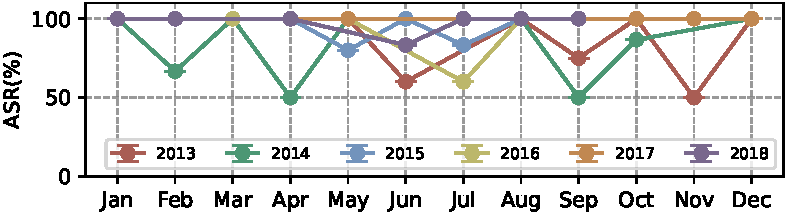
\includegraphics[width=\linewidth,keepaspectratio]{Graph/Evaluation/Figure9-update.pdf}
	\caption{Attack Persistence over 6 years }
	\label{fig:Attack Persistence-APIGraph}
\end{figure}

The effectiveness of the \pandora using the problem-space adversarial perturbation in poisoned sample generation has already been validated. 
Next, we evaluate the effectiveness of the concept drift direction misguidance.
We selected 138 families with less than six months of survival for comparative analysis. 
We divided the attack targets into five groups based on the duration of the attack test.
The results of the attack’s effectiveness are presented in Figure~\ref{fig:feature-space perturbation strategy}.
\begin{figure}[h!]
	\centering
	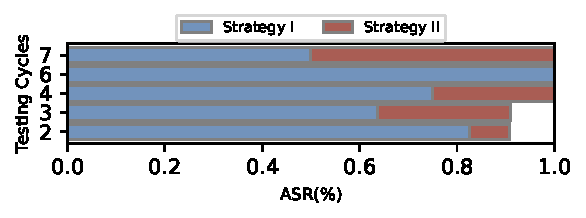
\includegraphics[width=\linewidth,keepaspectratio]{Graph/Evaluation/Figure26.pdf}
	\caption{Feature-space perturbation strategy}
	\label{fig:feature-space perturbation strategy}
\end{figure}
After introducing the concept drift misguidance based on the shapley additive explanations, the attack success rate improved for most targets, reaching an average of 91.3\%.
This represents a 10.9\% increase compared to the previous attack success rate achieved with the problem-space perturbation strategy.
The increase in ASR is due to the attacker’s ability to generate poisoned samples with higher uncertainty than those produced using the problem-space adversarial perturbation strategy.
After applying concept drift misguidance, the average uncertainty ranking of the poisoned samples increased by 66.2\%.
This further demonstrates the complementary roles of the two modules in the generation of poisoned samples by \pandora.

In addition, since computational cost is a primary concern in machine learning scenarios, the attacker’s model was weakened to reduce computational overhead.
Specifically, we weaken the model by reducing the number of neural network layers in the encoder or classifier.
Following state-of-the-art Android malware concept drift adaptation methods~\cite{2023-Usenix-chenyizhen}, which employ an encoder and classifier, we tested four weakened settings based on the victim model, as shown in Figure~\ref{fig:Attack-effectiveness-model-heterogeneity}.
ENC denotes the encoder, CAL represents the classifier, and W indicates a decrease in the model’s capacity, reflected in a reduction of model parameters.

\begin{figure}[h!]
	\centering
	\includegraphics[width=\linewidth,keepaspectratio]{Graph/Evaluation/Figure10_1.pdf}
	\caption{Attack Effectiveness under Weakened Capabilities}
	\label{fig:Attack-effectiveness-model-heterogeneity}
\end{figure}
\begin{figure*}[t]
	\centering
	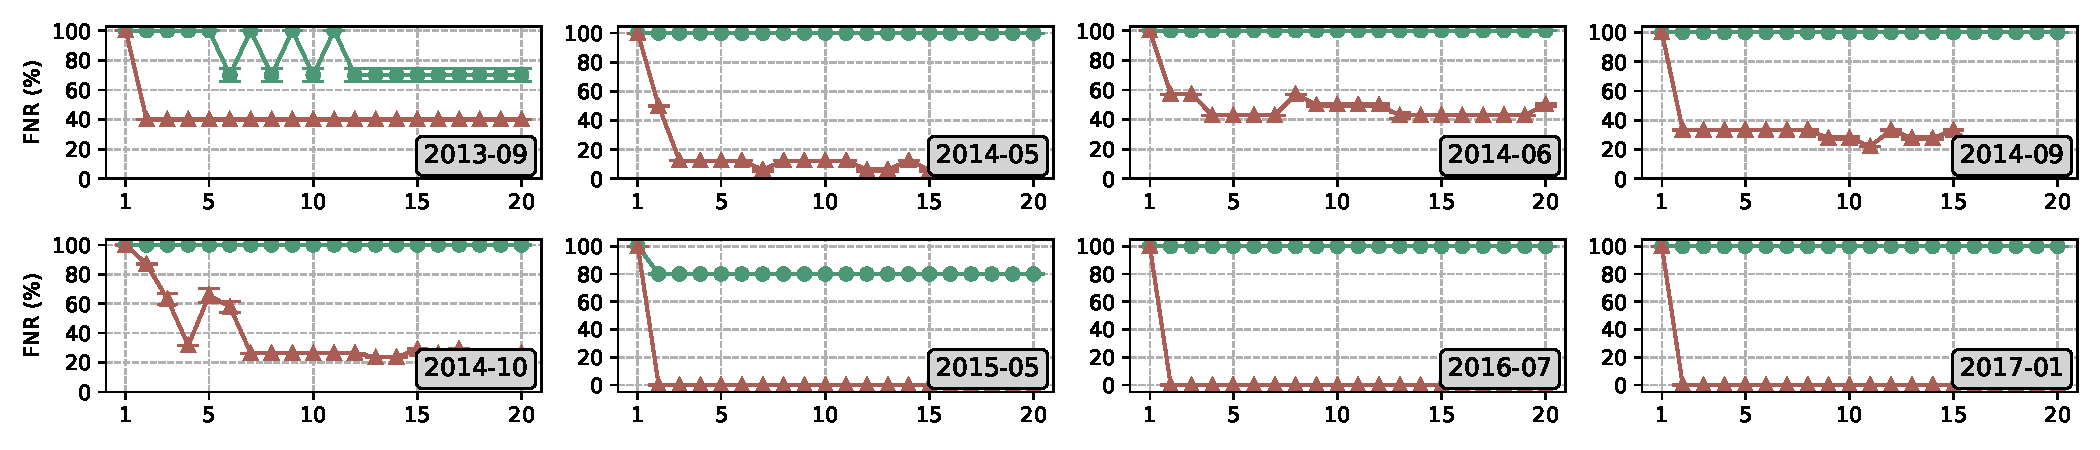
\includegraphics[width=\linewidth,keepaspectratio]{Graph/Evaluation/api_multi_attackers_fnr_1-up.pdf}
	\caption{Attack Effectiveness with Multi-Target Attack (6 year Attack Testing)}
	\label{fig: Attack Effectiveness with Multi-Target Attack}
\end{figure*}

Previous studies have shown that when the attacker’s capabilities are limited, the effectiveness of poisoning attacks decreases~\cite{2022-ACM-Computing-Survey-Threats-to-training}.
However, \pandora mitigates this issue, achieving an average attack success rate of 81.17\% with limited attacker capabilities, as shown in Figure~\ref{fig:Attack-effectiveness-model-heterogeneity}. 
We also found that weakening the encoder reduces the attack success rate by nearly 10\%, which is more significant than weakening the classifier.  
This indicates that the encoder part of the surrogate model plays a crucial role in approximating the capabilities of the victim model.
Additionally, we found that weakening both the encoder and the classifier in the attacker’s surrogate model does not result in the lowest attack success rate.
Under this configuration, the attack success rate is even higher than that of the setup where only the classifier is weakened, at 86\% compared to 83\%.
This phenomenon contradicts the expectation that attackers must invest more computational resources to achieve a higher attack success rate.
By analyzing the set of attack targets under different configurations, we found that when the surrogate model is weakened, its selection of attack targets is significantly biased.
In the synchronized weakening setting, only 55\% of the attack targets remain compared to the control group, highlighting the need to assess attack effectiveness under constrained attacker capabilities using ASR and the number of attack targets.
To address this issue, we define the Number of Successful Attack Targets (NSAT) and the Relative Attack Success Rate (RASR), which represents the ratio of successfully attacked targets in the weakened attacker’s setup to those in the control group, as shown in Equation~\ref{attack seed formula 1}.
\begin{equation}
	\begin{aligned}
		RASR = \small NSAT_{weak}/\small NSAT_{control}
	\end{aligned}
	\label{attack seed formula 1}
\end{equation}
As model capability weakens, RASR declines, with the weakest setup showing a 43.18\% drop.
While a reduced scope of attack targets weakens the attacker’s capabilities, the relative attack success rate increases, posing a significant threat to concept drift adaptation by enhancing resource utilization efficiency even under constrained conditions.

\subsubsection{Multi-Target (Attacker) Attack} 
\label{Sec: Multi Attack Targets}
As described in Section~\ref{Experimental Setup}, the multi-targets setting simulates two practical scenarios: (1) a single attacker launching attacks against multiple targets, and (2) multiple attackers independently targeting different targets.
For clarity and ease of analysis, we adopt the first scenario, where a single attacker conducts multi-target attacks, as the basis for the following discussion.
Multiple attack targets may emerge within the same concept drift cycle in real-world scenarios. 
Therefore, \pandora also supports a multi-target attack mode.
In the multi-target attack setting, the attacker performs \pandora on multiple attack targets simultaneously.
To evaluate the effectiveness of the \pandora in a multi-target setting, we selected 8 months with different attack targets for testing, covering a 6-year evaluation period, as illustrated in Figure~\ref{fig: Attack Effectiveness with Multi-Target Attack}.
For each multi-target setting, we conducted a 20-month attack test.
Detailed information on the settings can be found in Appendix~\ref{Sec: Attack Target List}.
The multi-target attack achieved an average success rate of 97.5\% across different testing times, demonstrating its effectiveness in executing the \pandora on multiple targets.
During the 80-month attack test, only the attack success rate in May 2015 was not 100\%, although it still maintained an effective success rate of 80\%.
The high attack success rate in a multi-target setting is due to the coverage effect of labeling budget consumption across different attack targets.
When multiple attack targets are present, once the labeling budget for the most uncertain attack target is exhausted, the labeling budget for the other attack targets is also concurrently depleted.
Consequently, the \pandora incurs a low cost, as a single attack benefits multiple targets simultaneously.

Then we discuss the scenario where multiple distinct attackers simultaneously target different attack targets.
In terms of attack effectiveness, the success rate in the multi-attacker setting is consistent with that in the single attacker setting with multiple attack targets.
This is because, as previously analyzed, the poisoned samples generated for different attack targets do not interfere with one another.
In fact, poisoned samples crafted for attack targets with the highest uncertainty can even facilitate the misclassification of other attack targets.
Furthermore, we observe that when attack effects are mutually beneficial, attackers tend to cooperate, thereby reducing the overall attack cost. Specifically, multiple attackers can identify the attack target with the highest uncertainty and use it as a common target, allowing them to share the costs involved in poisoned sample generation.
%接下来我们讨论多个不同攻击者对不同攻击目标同时进行攻击的情况。
%在攻击效果方面,多攻击者的攻击成功率与单一攻击者攻击多个目标设置下的攻击成功率是一样的。
%因为如上述分析所示,针对不同攻击目标生成的投毒样本彼此之间不会产生相互干扰,反而是具有最高不确定性的攻击目标生成的投毒样本可以辅助其他攻击目标成功实现误分类的攻击效果。
%并且我们发现在攻击效果可以彼此收益的情况下,攻击者之间会倾向于相互合作,进而降低整体的攻击成本。
%因为多个不同的攻击者可以选出攻击目标中不确定性最高的样本作为群体攻击目标,进而分摊投毒样本生成过程中的各种开销。
\begin{table}[h!]
	\caption{Multi-Target Attack across Four Ddatasets}
	\label{tab: asz }
	\setlength{\tabcolsep}{5.8pt}
	\begin{center}
		\scalebox{1.0}{
			\begin{tabular}{ccccc}
				\toprule
				\textbf{Datasets}&\textbf{Targets}&\textbf{F1-Testing} &\textbf{F1-Validation} &\textbf{ASR (\%)} \\
				\midrule
				APIGraph & 331  &  0.76\textsubscript{\textcolor{black}{-0.15}} & 0.99 & 92.92\% \\ 
				\specialrule{0.05em}{1pt}{1pt}
				MNIST & 1,398  & 0.78\textsubscript{\textcolor{black}{-0.12}} & 0.99 & 79.98\%\\
				\specialrule{0.05em}{1pt}{1pt}
				BODMAS & 222  &  0.92\textsubscript{\textcolor{black}{-0.06}}& 0.92 &80.63\% \\ 
				\specialrule{0.05em}{1pt}{1pt}
				SPAM & 168  &  0.91\textsubscript{\textcolor{black}{-0.07}} & 0.99 &74.40\% \\ 
				\bottomrule
		\end{tabular}}
	\end{center}
\end{table}

In certain special cases, the attacker may need to target all attack targets simultaneously.
This represents a special scenario within multi-target attacks.
Therefore, we tested the effectiveness of \pandora on all attack targets at different concept drift time points.
The average attack success rate reaches 81.98\% (as shown in Table~\ref{tab: asz }), with a notably high success rate of 92.92\% achieved on the real-world concept drift dataset, APIGraph.  
Moreover, we observe that the victim models maintain high F1 scores on the initial validation set under attack across different datasets, with an average of 0.99.
This demonstrates that our method preserves the victim model’s previously learned knowledge, even when targeting all attack targets, thereby highlighting the stealth of the proposed attack.
The impact on test performance (F1-Testing) varies across datasets, reflecting how limited access to new samples can hinder the model’s adaptation to concept drift.
The performance degradation on the BODMAS and SPAM datasets is relatively minor, with average F1-score drops of less than 0.07, indicating a lower intensity of concept drift in these scenarios.
In contrast, the APIGraph and MNIST datasets exhibit more substantial performance changes, with average F1-score drops of around 0.14.
This suggests stronger concept drift and a higher reliance on the victim model for effective learning from drifted samples.
Nevertheless, \pandora stealth remains unaffected in both cases, as the testing data is unlabeled, and the victim model cannot promptly detect its performance degradation.

\subsection{Attack Influencing Factors}
\label{Sec: Attack Influencing Factors}

We have demonstrated the effectiveness of \pandora.
To further investigate how real-world conditions affect attack performance, we analyze the factors influencing \pandora using a real-world Android malware dataset (APIGraph~\cite{2020-CCS-APIGraph}) spanning seven years.

\subsubsection{Impact of Different CDA-AL Strategies}
Existing concept drift adaptation strategies in sensitive domains~\cite{2023-Usenix-chenyizhen,2022-SP-Trancending,2021-Usenix-CDAE} can be broadly categorized into four types. 
In addition to the uncertainty-based strategies discussed in Section~\ref{Sec: Concept Drift Adaptation}, the remaining approaches fall into three categories. 
To ensure the generality of our findings, we evaluate the effectiveness of \pandora across all these representative adaptation strategies.

\begin{itemize}[leftmargin=0.35cm]

\item CADE~\cite{2021-Usenix-CDAE} trains an encoder with labeled data to learn compressed input representations. 
It uses a distance function to identify concept drift samples that deviate from the training data.
\begin{equation}
	\begin{aligned}
		d_{i} = ||\bm{\mathrm{z}}_{i}-\bm{\mathrm{zc}}_{i}||_{2} \\
	\end{aligned}
	\label{CADE}
\end{equation}
Specifically, $\bm{\mathrm{z}}_{i}$ represents the latent space embedding of the sample $\bm{\mathrm{x}}_{i}$ obtained from the encoder. 
A sample is a concept drift instance if its distance $d_{i}$ to the nearest training sample in the encoder’s latent space exceeds a predefined threshold.
\item TRANS~\cite{2022-SP-Trancending}
applies conformal prediction~\cite{2005-high-cite-Algorithmic-learning-in-a-random-world} to concept drift adaptation.
It calculates a testing sample’s non-conformity score, credibility (proportion of calibration samples with higher scores), and confidence (1 minus the opposite label’s credibility). 
Low scores indicate potential drift.
\item HCL~\cite{2023-Usenix-chenyizhen}
proposes the latest concept drift adaptation strategy, combining an encoder and classifier. 
Its training loss $\mathcal{L}(\bm{\mathrm{x}}_{i})$ integrates hierarchical contrast loss $\mathcal{L}_{hc}(\bm{\mathrm{x}}_{i})$ and classification loss $\mathcal{L}_{ce}(\bm{\mathrm{x}}_{i})$.
\begin{equation}
	\begin{aligned}
		\mathcal{L}(\bm{\mathrm{x}}_{i}) = \mathcal{L}_{hc}(\bm{\mathrm{x}}_{i}) + \mathcal{L}_{ce}(\bm{\mathrm{x}}_{i}) \\
	\end{aligned}
	\label{CADE}
\end{equation}
Samples with higher loss values are more likely to be affected by concept drift, as different samples incur different loss levels during inference.

\end{itemize}
%The evaluation includes both traditional model uncertainty approaches and concept drift adaptation strategies that leverage advanced machine learning techniques, such as contrastive learning.
%As shown in Figure~\ref{fig:Attack-effectiveness-Concept-Drift-Strategy}, the experimental results demonstrate that our attack consistently achieves an attack success rate exceeding 80\% across four various concept drift adaptation strategies.
%Furthermore, during the attack process, the performance metrics of the primary task remain stable, with the F1 consistently exceeding 0.88 across all strategies.
%Notably, the ASR reaches 92.77\% when targeting the currently optimal concept drift adaptation method (HCL).
%The primary reason \pandora achieves the highest attack success rate on HCL is that HCL selects concept drift samples based on their loss function values, making the constructed poisoned samples significantly impact the retraining process of the victim model.
%As a result, ensuring the security of concept drift adaptation methods has become an urgent challenge requiring immediate attention.
% Version
%The evaluation includes traditional uncertainty-based approaches and advanced concept drift adaptation strategies, such as contrastive learning.
%As shown in Figure~\ref{fig:Attack-effectiveness-Concept-Drift-Strategy}, \pandora achieves an ASR exceeding 80\% across all four strategies while maintaining stable primary task performance, with F1 consistently above 0.88.
%Notably, \pandora achieves a 92.77\% ASR against the optimal concept drift adaptation method (HCL).
\begin{figure}[h!]
	\centering
	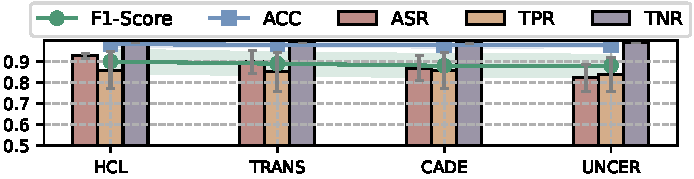
\includegraphics[width=\linewidth,keepaspectratio]{Graph/Evaluation/Figure13.pdf}
	\caption{Different Concept Drift Adaptation Strategies}
	\label{fig:Attack-effectiveness-Concept-Drift-Strategy}
\end{figure}
The evaluation covers traditional uncertainty-based methods and advanced concept drift strategies like contrastive learning.
As shown in Figure~\ref{fig:Attack-effectiveness-Concept-Drift-Strategy}, \pandora achieves over 80\% ASR across all four strategies while maintaining F1 scores above 0.88.
\pandora attains a 92.77\% ASR against the latest adaptation method (HCL).
%These results highlight the urgent need to address security challenges in concept drift adaptation methods.

%\begin{figure}[h!]
%	%\vspace{-0.8em}
%	\centering
%	\subfloat[Different Strategies]{
%		\label{fig11-1}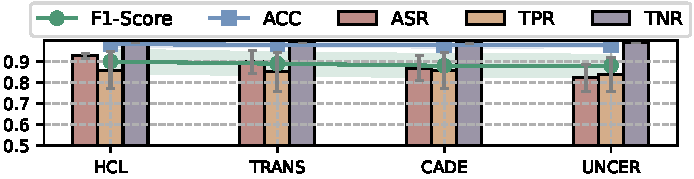
\includegraphics[width=4.25cm, height=2.9cm]{Graph/Evaluation/Figure13.pdf}
%	}
%	\subfloat[Labeling Budget]{
%		\label{fig11-2}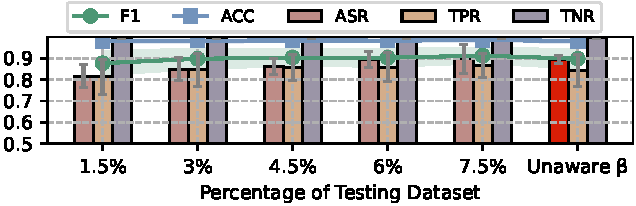
\includegraphics[width=4.25cm, height=2.9cm]{Graph/Evaluation/Figure14_3.pdf}
%	}
%	\caption{xxxxxxxxxxxxx.} 
%	\label{fig111}
%	%\vspace{-1em}
%\end{figure}

\subsubsection{Impact of Labeling Budget}
\label{Sec: Attack Effectiveness under Different Label budget}
The labeling budget represents the cost of manual labeling and is one of the most valuable resources in CDA-AL.
We evaluated the attack effectiveness under six different labeling budget settings.
Each labeling budget setting represents its proportion of the testing data, following the settings of existing studies~\cite{2023-Usenix-chenyizhen}.
The first five labeling budget settings assume the attacker knows the victim model’s labeling budget.
In contrast, the last setting assumes the attacker cannot access the victim model’s labeling budget.
When the attacker is unaware of the labeling budget settings, poisoned samples are generated based on the maximum computational capacity of the attacker. 
In this experiment, we set the attacker’s capacity four times the potential labeling budget computation capacity.
\begin{figure}[h!]
	\centering
	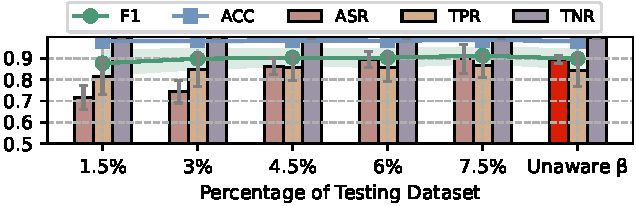
\includegraphics[width=\linewidth,keepaspectratio]{Graph/Evaluation/Figure14_4.pdf}
	\caption{\pandora Under Different Labeling Budget}
	\label{fig:Attack-effectiveness-Label-Budget}
\end{figure}
As shown in Figure~\ref{fig:Attack-effectiveness-Label-Budget}, \pandora remains effective across budgets, with an average attack success rate of 85.10\%.
Even without access to the victim model’s labeling budget, the attacker can still achieve a high attack success rate by leveraging the maximum available resources, reaching 89.33\%.
The high attack success rate, even without access to detailed labeling budget information, is due to the significantly lower cost of poisoning attacks than the victim’s concept drift adaptation cost, which is primarily driven by labeling expenses.
Thus, the attacker can generate as many poisoned samples as possible to consume the victim model’s labeling budget.
This strategy is inspired by DDoS~\cite{mirkovic2004taxonomy} attacks, where the attacker maximizes attack traffic without knowing the victim’s total resources to achieve the attack objective.
Moreover, even if the scale of poisoned samples in the \pandora attack exceeds the labeling budget, it is unlikely to raise suspicion.
This is because the poisoned samples are injected into the unlabeled testing data stream during each concept drift cycle, and the volume of this stream is substantially larger than the victim model’s monthly labeling budget.
As a result, \pandora exhibits strong stealth. 
Furthermore, it is extremely difficult for the victim model to detect poisoned samples within the testing data stream due to the massive volume of incoming data, which makes full inspection infeasible.

%In our setup, the label budget reflects a victim model’s real-world capabilities.\footnote{According to Kaspersky’s 2023 statistics~\cite{Kaspersky-Android-Malware-Threat-Statistics}, the total number of Android malware samples for the year reached 1.12 million. Using the commonly assumed 9:1 ratio of benign to malicious samples, the total number of benign and newly detected malicious samples per month is estimated to be 11.2 million.}
%The maximum budget of 300 samples represents approximately 9\% of the monthly test data, which is equivalent to the manual analysis of 83,761 samples each month in real-world scenarios.
%An estimated cost of 22 USD per sample (obtained through interviews with security vendors) translates to 1.84 million USD per month, representing a substantial financial burden for security companies.

%\subsubsection{Impact of Data Collection Capability}
%In multi-target attacks, there is a special case where the attack target consists of all the test data.
%In this case, the attacker’s poisoning seed samples need to be the highest uncertainty samples from the test dataset, making data collection capability crucial to its effectiveness.
%So we conducted attack experiments with five settings on four datasets.
%\pandora relies on identifying high-uncertainty attack seeds to generate poisoned samples.
%The uncertainty of these seeds is influenced by the attacker’s data collection capabilities, affecting the overall attack effectiveness.
%Tests were conducted across four datasets under different data collection capacities to analyze their effects on attack performance, as illustrated in Figure~\ref{fig:Impact of Data Collection Ability}.
%\begin{figure}[t]
%	\centering
%	\includegraphics[width=\linewidth,keepaspectratio]{Graph/Evaluation/figure17-v3.pdf}
%	\caption{Impact of Data Collection Ability}
%	\label{fig:Impact of Data Collection Ability}
%\end{figure}
%No clear correlation was observed between reduced data collection capability and diminished attack effectiveness.
%Across all four datasets, reduced data collection sometimes improved attack performance. 
%For instance, in the MNIST dataset, attacks with 90\% data collection capability outperformed those with 100\% capability in over 80\% of the attack test cycles.
%Similarly, in the APIGraph~\cite{2020-CCS-APIGraph} dataset, 50\% capability occasionally surpassed 100\% in specific periods.
%The above analysis shows that attack effectiveness relies more on the presence of high-uncertainty samples than on data collection capability alone.
%Even when there are differences in data quantity and distribution between the attacker and the victim model, attackers can still achieve significant success by acquiring such samples.

\subsubsection{Impact of Feature Selection}
\label{Impact of Feature Selection}
Both APIGraph and Androzoo are Android malware datasets designed to capture concept drift. By comparing the differences in attack performance between these two datasets, we analyze how variations in feature construction affect the attack effectiveness.
Since APIGraph employs a more advanced feature extraction method, we selected the classic DREBIN~\cite{2014-NDSS-drebin} approach for feature extraction on the Androzoo dataset.
Experiments show that \pandora still achieves strong performance, with an attack success rate over 90\%.
Moreover, compared to the no-attack setting, the victim model shows only a 0.01 change in F1 score and less than 1.5\% variation in FNR, indicating strong stealthiness of the attack.
The ability of \pandora to achieve a high attack success rate under various feature selection methods demonstrates the robustness and generalizability of our attack strategy.

On AndroZoo, the multi-target ASR averaged 81\%, confirming PANDORA’s effectiveness, though lower than the 97.5\% on APIGraph, indicating that drift intensity and feature extraction affect attack performance.

\subsubsection{Impact of Problem-Space Perturbations}
\label{Impact of Problem-Space Perturbationsn}
Table 1 shows cheap problem-space perturbations; other strategies are also viable. Our supplementary tests (AndroZoo) with six perturbation strategies preserved Drebin features and achieved a 90\% ASR, demonstrating PANDORA’s robustness.

\subsubsection{Impact of Incomplete Test Data}
\label{Impact of Incomplete Test Data}
With 30\%, 50\%, or 70\% of test data, success averages 75.6\% (APIGraph, single-target). Poisoned samples use high-uncertainty benign seeds found without full distribution knowledge.

\subsubsection{Impact of Unknown Uncertainty Strategy}
\label{Impact of Unknown Uncertainty Strategy}
Without uncertainty estimates, PANDORA transfers via confidence approximations.
On APIGraph, attacks on HCL and CADE with UNCER achieve 75\% ASR, as different strategies give similar rankings for sample selection.

\subsection{Ablation Study}
To effectively demonstrate the importance of each component in \pandora, we conduct ablation studies by removing key elements of the attack pipeline.
This allows us to evaluate the necessity of each component and analyze the underlying factors contributing to \pandora’s success.
\begin{table}[h!]
	\caption{Attack value assessment necessity analysis}
	\label{tab: Attack Value Assessment necessity analysis}
	\setlength{\tabcolsep}{5.8pt}
	\begin{center}
		\scalebox{0.9}{
			\begin{tabular}{ccc}
				\toprule
				\textbf{Ablation Component}&\textbf{Ablation-ASR (\%)}&\textbf{ASR (\%)} \\
				\midrule
				Poisoning Ratio Estimation & 10.87  &  89.22\textsubscript{\textcolor{red}{\textbf{+78.35}}} \\
				\specialrule{0.05em}{1pt}{1pt}	
				Constraint Search for Poisoning Seed & 10.99  &  89.22\textsubscript{\textcolor{red}{\textbf{+78.93}}} \\
				\specialrule{0.05em}{1pt}{1pt}
				Poisoned Sample Generation & 10.87  &  89.22\textsubscript{\textcolor{red}{\textbf{+78.35}}} \\
%				CADE (Data Based) & 72.43\textsubscript{\textcolor{ForestGreen}{\textbf{-14.47}}}  & 86.90 \\
				\bottomrule
		\end{tabular}}
	\end{center}
\end{table}
As described in Section~\ref{Sec: Attack Method}, the \pandora framework consists of three main components.
Our ablation study focuses on analyzing the impact of these three core components.
We conduct the ablation study on the APIGraph concept drift dataset~\cite{2020-CCS-APIGraph}, which features the longest duration of concept drift.
%\subsubsection{Impact of Attack Value Assessment}
%Analyzing the attack value of attack targets provides crucial support for the \pandora.
%To demonstrate the significance of this step, we conduct ablation experiments where attackers skip the attack value assessment phase and proceed directly to poisoning seed sample selection and poisoned sample generation.
%This approach implies that attackers target all new malware, leading to a significant increase in attack cost.
%\begin{table}[h]
%	\centering
%	%	\renewcommand{\arraystretch}{0.9}  % 调整表格的行距
%	\small
%	\caption{Attack value assessment necessity analysis}
%	\label{tab: Attack Value Assessment necessity analysis}
%	%\renewcommand{\arraystretch}{0.75}  % 调整该表格的行距
%	\begin{tabular}{ccc}
%		\toprule
%		% \textbf{Setting} & \textbf{Ablation-ASR} & \textbf{ASR} & \textbf{Improvement} & \textbf{Sample Reduction} \\
%		\textbf{Stratege} & \textbf{Ablation-ASR (\%)} & \textbf{ASR (\%)}\\
%		\midrule
%		HCL (Model Based) & 81.73 & \textbf{92.77}\textsubscript{\textcolor{red}{\textbf{+11.04}}}\\
%		CADE (Data Based) & 72.43 & \textbf{86.90}\textsubscript{\textcolor{red}{\textbf{+14.47}}}\\
%		%UNCER & 61.50 & \textbf{82.86}\textsubscript{\textcolor{red}{\textbf{+21.36}}}\\
%		\bottomrule
%	\end{tabular}
%\end{table}
%Existing concept drift adaptation strategies are primarily divided into data-driven and model-driven approaches.
%Therefore, in the attack value assessment module, we selected two representative strategies, CADE and HCL, from each category for evaluation. 
%For the labeling budget, we chose a medium-level sample labeling capacity and set the labeling budget to 200.
%Removing the attack value assessment module causes \pandora to indiscriminately target all emerging malware families without prioritization.
%Experimental results show an average 15.62\% drop in attack success rate, underscoring the critical importance of this component in ensuring attack effectiveness.
%Moreover, indiscriminately expanding the set of attack targets significantly increases the overall attack cost.
As shown in Table~\ref{tab: Attack Value Assessment necessity analysis}, when the attacker lacks poisoning ratio analysis, they cannot determine the number of required poisoned samples.
As a result, seed samples are directly injected into the testing stream.
Due to the limited number of poisoned samples, the labeling budget is not effectively consumed, reducing the attack success rate to 10.87\%.
Disabling the poisoned seed search forces the attacker to randomly perturb testing samples, resulting in poisoned data with low uncertainty.
This weakens labeling budget consumption, yielding an attack success rate of 10.99\%.
Finally, without the poisoned sample generation module, the attacker fails to produce samples aligned with labeling budget consumption requirements, again causing a drop in success rate to 10.87\%.
	
	\section{Potential Defenses}
\label{Sec: Potential Defenses}
CDA-AL methods lack directly relevant and effective defenses against poisoning attacks.
While Lin et al.~\cite{2021-GLOBALCOM-acctive-learning-under-malicious-mislabeling-poisoning-attacks} proposed defenses for active learning poisoning attacks based on static unlabeled and clean datasets. 
However, these assumptions break down in CDA-AL, where unlabeled data evolves and clean datasets quickly become outdated.
Therefore, we evaluated \pandora against three representative targeted poisoning attack defense mechanisms~\cite{chen2018detecting,DFP,2023-ICCV-Trigger-Detect}.
The three methods correspond to the three possible stages at which defenses can be deployed within the CDA-AL framework. 

\begin{itemize}[leftmargin=0.35cm]
	\item \textbf{Data Sanitization (Data Processing)}: activation clustering~\cite{chen2018detecting} (AC) is a data inspection method that assumes poisoned data forms a distinct cluster within the target class, either small or distant from the class center.
	
	\item \textbf{Input-Time Detection (Sample Selection)}: Liu et al.~\cite{2023-ICCV-Trigger-Detect} observed that targeted poisoning attacks often embed triggers into attack targets to induce misclassification.
	However, such triggered samples exhibit consistent corruption robustness (CRC) under input perturbations. Leveraging this observation, they proposed detecting targeted poisoning attacks by analyzing robustness variations.
	
	\item \textbf{Robust Training (Model Retraining)}: Data-Free Pruning~\cite{DFP} (DP) defends against data poisoning attacks by pruning neurons that remain dormant for clean data, based on the assumption that poisoned and clean samples activate different subsets of neurons.
	
%	\item \textbf{Fine-Tuning (FT)}~\cite{FT} can mitigate targeted poisoning attacks, but it requires labeled training dataset to avoid overfitting.
	
%	\item  \textbf{Fine-Pruning (FP)}~\cite{FP} mitigates poisoned models by pruning neurons dormant on clean validation data, measuring average neuron activation, and removing the least active ones. 
\end{itemize}
%\begin{table}[t]
%	\caption{Existing Defenses Against \pandora} %标题
%	\label{tab: Analysis of Existing Defenses Against Poisoning Attacks (TPA)} %表标签
%	\centering
%	\renewcommand{\arraystretch}{0.9}  % 调整表格的行距
%	\small
%	\begin{tabular}{|c|c|c|}
%		\hline
%		\textbf{Method}  & \textbf{F1-score} & \textbf{Avarage ASR Decrease (268 Months)}  \\ \hline
%		AC~\cite{AC} & 0.90 &  16.5\%\\ \hline
%		DFP~\cite{DFP}   & 0.87 & 21.8\%  \\ \hline
%		FT~\cite{FT}   & - & without extensive labeled training dataset   \\ \hline
%		FP~\cite{FP}   & - & without clean labeled validation dataset   \\ \hline
%		ICDF(Our) & 0.90 &  \textbf{39\%}  \\ \hline
%	\end{tabular}
%\end{table}

Defenses based on feature separability (AC) and model parameter adjustments (DFP) are applicable, but their defensive effectiveness is limited.
As shown in Figure~\ref{fig:ICDF Defense Motivation}, t-SNE
visualization reveals that \pandora's use of attack seeds creates intricate entanglement between poisoned and clean samples in the
feature space (the APIGraph dataset's test data from June 2013).
As a result, existing defenses cannot distinguish between clean and poisoned samples, so they cannot fully defend against \pandora attacks.
\begin{figure}[h!]
	\centering
	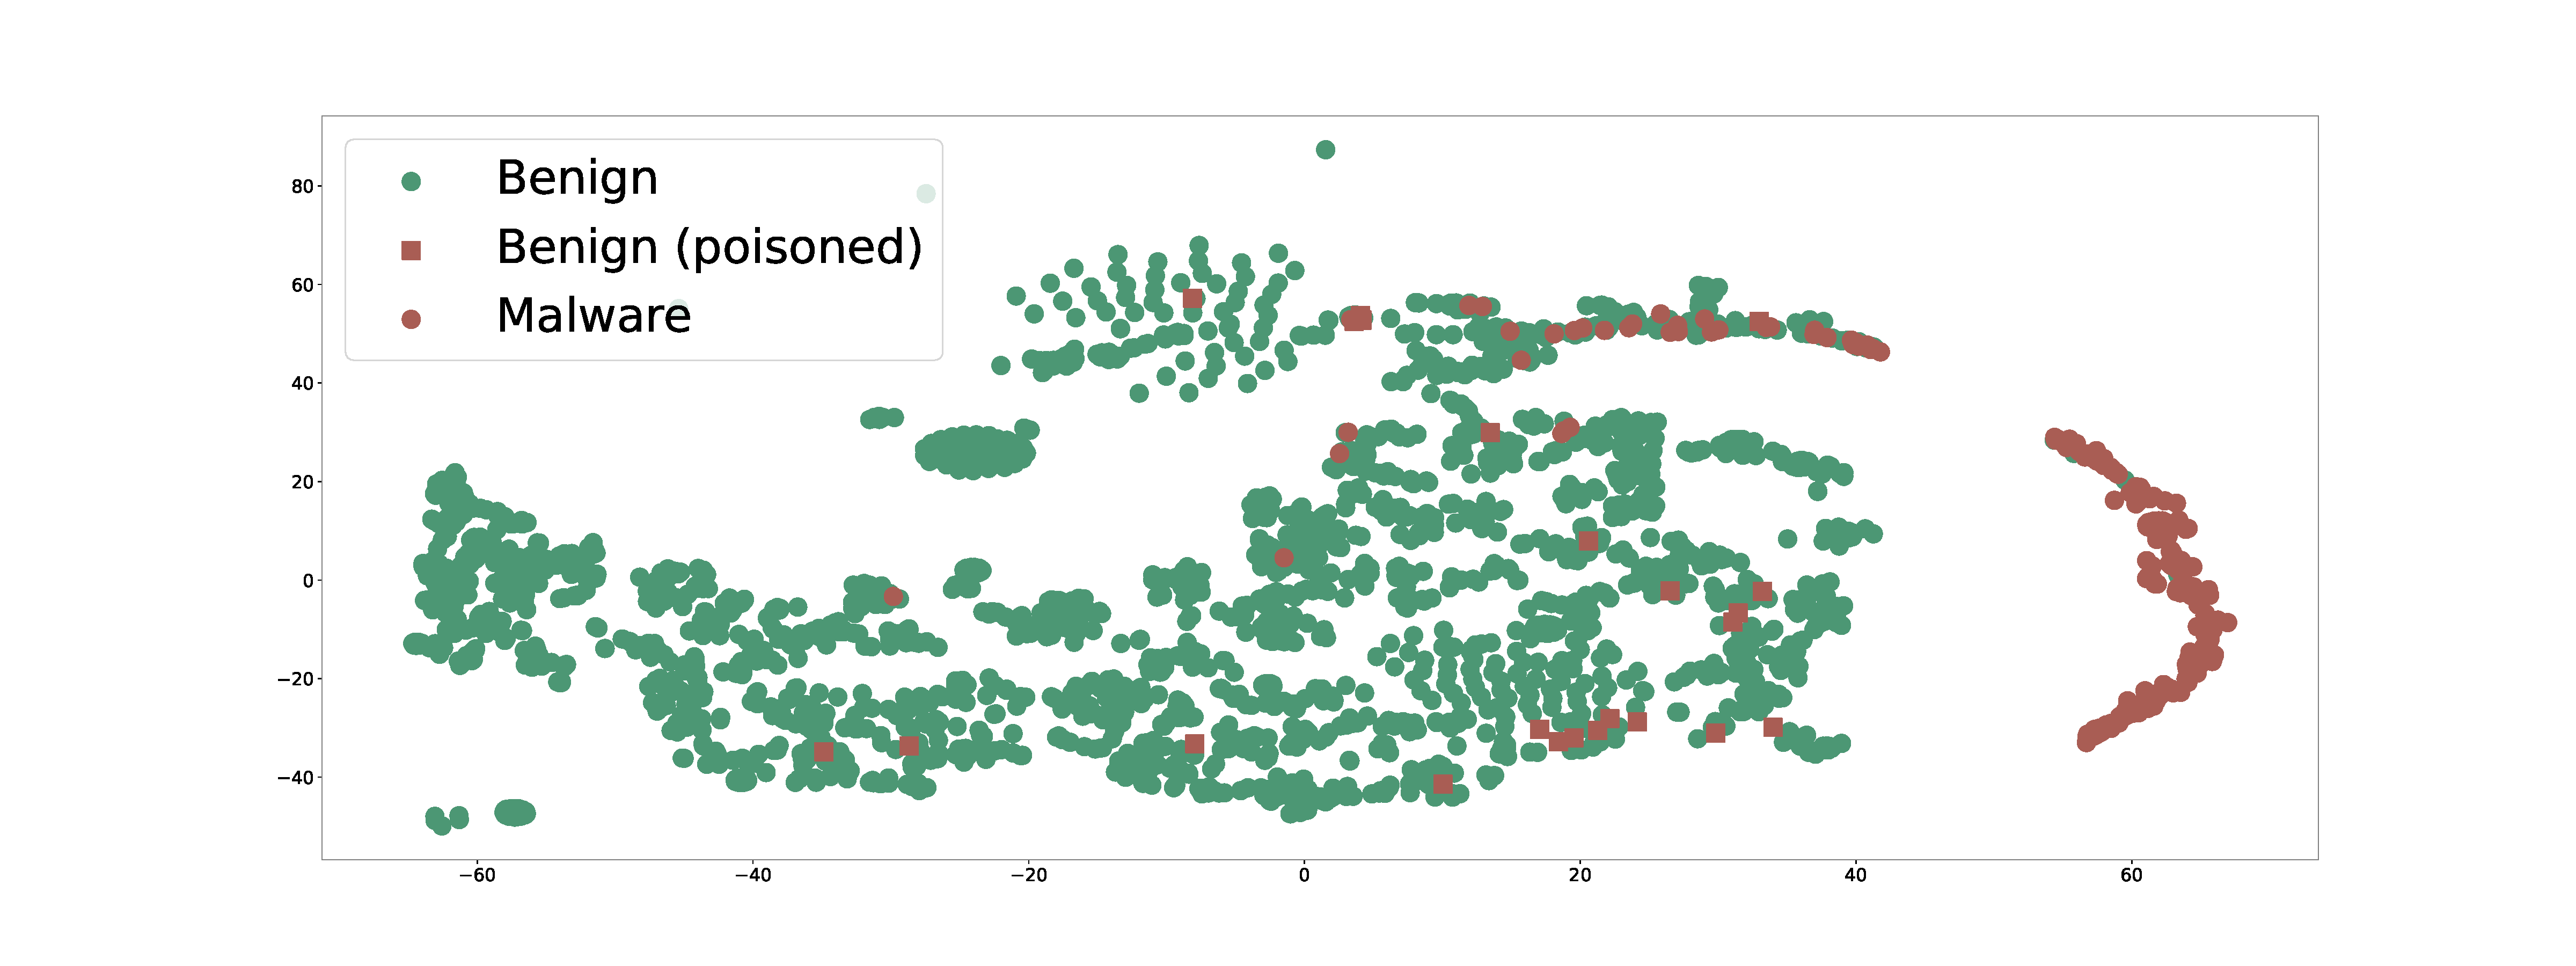
\includegraphics[width=\linewidth,keepaspectratio]{Graph/Evaluation/Figure20.pdf}
	\caption{ICDF Defense Motivation}
	\label{fig:ICDF Defense Motivation}
\end{figure}
Thus, the attack success rate decreases by less than 20\% on average. Specifically, the ASR drops by 16.5\% under the AC defense and 21.8\% under DFP.
Given these limitations, we explore alternative defense strategies in countering \pandora.

Intra-Cluster Distance Filtering (ICDF): In the \pandora, the attacker relies on poisoning seed samples to generate poisoned samples, reducing costs and leading to similarity among the poisoned samples.
Different poisoned samples may originate from the same seed sample.
We measure this similarity using Euclidean distance in the feature space, the basis for our defense method (ICDF).
Unlike AC-based defenses, ICDF filters poisoned samples by exploiting the similarities between the poisoned samples themselves.
%Motivated by this observation, we propose an adaptive sample filtering method based on intra-cluster distance.
%Unsupervised clustering algorithms (e.g., K-means) are applied to the concept drift samples, partitioning the data into $\mathcal{C}$ clusters.
%Each cluster $c \in \mathcal{C}$ contains multiple concept drift samples, and the intra-cluster distance threshold $\tau$ is determined by calculating the mean Euclidean distance between any two samples within the same cluster.
%For each cluster $c$, samples with distances to other samples smaller than the cluster-specific threshold $\tau$ are removed.
So, we propose an adaptive sample filtering method based on intra-cluster distance.
Specifically, using an unsupervised clustering algorithm (e.g., K-means), we partition the concept drift samples into a set of clusters $Clu$ ($Clu= \{c_{1},c_{2},..,c_{k} \}$).
Each cluster $c_{k}$ calculates an intra-cluster distance threshold $\tau$ (Equation~\ref{ICDF Defense Method}) as the mean Euclidean distance $d_{Euc}(\bm{\mathrm{x}}_{i}, \bm{\mathrm{x}}_{j})$ between its samples.
\begin{equation}
	\begin{aligned}
		\tau = \frac{1}{|c_{i}| (|c_{i}| - 1)} \sum_{i \neq j} d_{Euc}(\bm{\mathrm{x}}_{i}, \bm{\mathrm{x}}_{j}) \quad i,j \in c_{k}
	\end{aligned}
	\label{ICDF Defense Method}
\end{equation}
$|c_{i}|$ is the number of samples in the cluster $c_{i}$.
Samples with distances smaller than $\tau$ to others in the same cluster are removed.
%\begin{figure}[t]
%	\centering
%	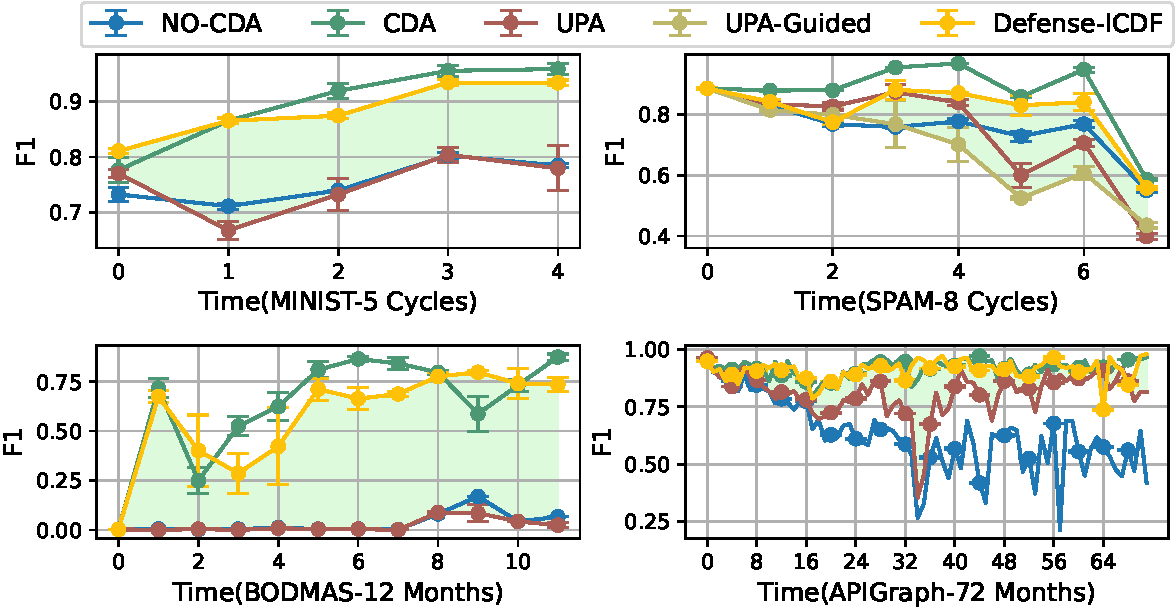
\includegraphics[width=\linewidth,keepaspectratio]{Graph/Evaluation/Figure19_1.pdf}
%	\caption{ICDF Defense (Multi-Target \pandora)}
%	\label{fig:ICDF Defense against Untargeted Poisoning Attack}
%\end{figure}
%\begin{figure}[h!]
%	%\vspace{-0.8em}
%	\centering
%	\subfloat[ICDF Defense Single-Target]{
%		\label{fig11-1}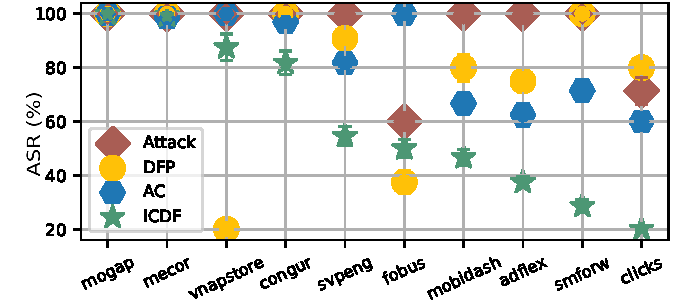
\includegraphics[width=3.90cm, height=2.9cm]{Graph/Evaluation/Figure-last_1.pdf}
%	}
%	\subfloat[ICDF Defense Multi-Target ]{
%		\label{fig11-2}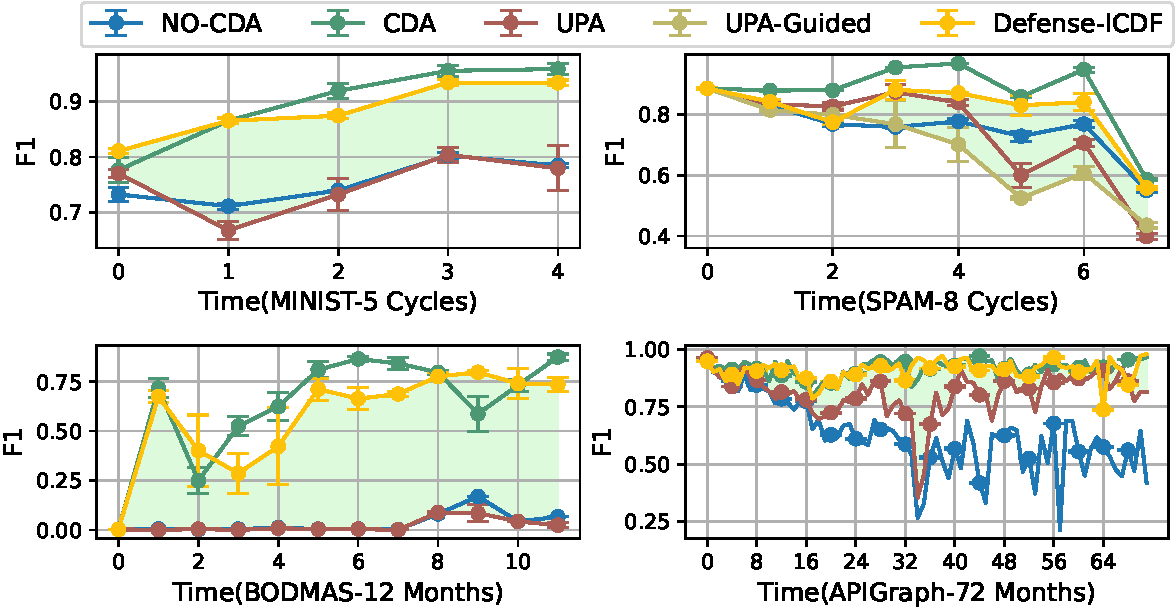
\includegraphics[width=4.60cm, height=2.9cm]{Graph/Evaluation/Figure19_1.pdf}
%	}
%	\caption{xxxxxxxxxxxxx.} 
%	\label{fig111}
%	%\vspace{-1em}
%\end{figure}
%The defense effectiveness against UPA is shown in Figure~\ref{fig:ICDF Defense against Untargeted Poisoning Attack}, demonstrating that the proposed defense method is effective across all four datasets.  
%For clarity, we used green shading to indicate the portion of model performance improvement after applying the ICDF defense method compared to the model performance under attack.
%Notably, in the MNIST and BODMAS datasets, the model performance during certain testing periods even exceeded the optimal performance of concept drift adaptation.  
%This demonstrates that our defense method not only filters out poisoned samples but also enhances the performance of concept drift adaptation itself.
%Among the datasets, the BODMAS dataset exhibited the greatest improvement, with an average F1 increase of 0.52 and a maximum increase of 0.78.
%\textbf{The ICDF defence effectively counters multi-target attack across all four datasets.}
%Green shading highlights performance improvements after applying ICDF, with notable gains in MNIST and BODMAS, where model performance during some periods surpassed the optimal performance of concept drift adaptation.
%The superior performance over the best original concept drift adaptation is due to ICDF's clustering approach, which removes poisoned samples and reduces data redundancy in clean samples, improving training efficiency.
%Although there is a lack of research in the concept drift field, studies in computer vision have shown that data redundancy reduces model training efficiency~\cite{kong2023peeling}.
%Since improving concept drift adaptation is beyond the scope of this study, we will address it in future research.
\begin{figure}[h!]
	\centering
	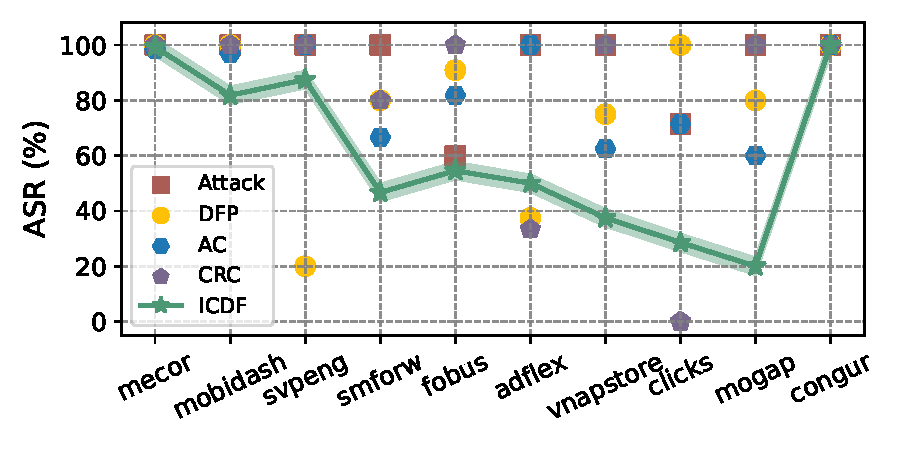
\includegraphics[keepaspectratio,height=3.5cm]{Graph/Evaluation/Figure-last.pdf}
	\caption{ICDF Defense (Single-Target \pandora)}
	\label{fig:APIGraph-targeted-defense}
\end{figure}
ICDF achieved the best defense effect under single-target attack mode, reducing the success rate of \pandora by 39\% across the Top 10 target sets, as shown in Figure~\ref{fig:APIGraph-targeted-defense}. 
While other defense methods demonstrated some effectiveness, they were 20.29\%, 12.43\% and 22.43\% less effective than ICDF, respectively.
We observed that, with the exception of ICDF, which consistently reduced the attack success rate across all attack targets, other defense methods inadvertently increased the attack success rate for certain targets.
%In the fobus family, the other three defense methods resulted in an average increase of 51.72\% in the attack success rate.
Moreover, ICDF effectively reduces the attack success rate of \pandora while causing only a 0.03 drop in F1-score compared to the no-attack scenario, thereby maintaining stable overall concept drift adaptation performance.
We also conducted defensive testing under an enhanced attack strategy that introduces misleading concept drift.
The attack success rate was reduced by 32.6\%, under the same experimental settings as those used in the attack effectiveness evaluation.
We also conducted defense tests against multi-target attacks across four different datasets, as shown in Table~\ref{tab:dma }.
The attack success rate decreased by an average of 54.97\% across the four datasets.
Therefore, our ICDF defense method also demonstrates strong effectiveness in defending against multi-target attack scenarios.
Moreover, after introducing the ICDF defense method, the F1 score on the four datasets was restored to an average of 0.91, indicating that the normal concept drift adaptation performance was not affected.
\begin{table}[htbp]
	\caption{ICDF Defense (Multi-Target \pandora)}
	\label{tab:dma }
	\setlength{\tabcolsep}{5.8pt}
	\begin{center}
		\scalebox{1.0}{
			\begin{tabular}{ccccc}
				\toprule
				\textbf{Datasets}&\textbf{Targets}&\textbf{F1-Attack} &\textbf{F1-Defense} &\textbf{ASR-Decrease} \\
				\midrule
				APIGraph & 734  &  0.76 & 0.90\textsubscript{\textcolor{red}{\textbf{+0.14}}} & 21.26\% \\ 
				\specialrule{0.05em}{1pt}{1pt}
				MNIST & 1,398  & 0.78 & 0.82 \textsubscript{\textcolor{red}{\textbf{+0.04}}}& 75.47\%\\
				\specialrule{0.05em}{1pt}{1pt}
				BODMAS & 222  &  0.92 & 0.99\textsubscript{\textcolor{red}{\textbf{+0.07}}} &54.05\% \\ 
				\specialrule{0.05em}{1pt}{1pt}
				SPAM & 168  &  0.91 & 0.94\textsubscript{\textcolor{red}{\textbf{+0.03}}} &69.04\% \\ 
				\bottomrule
		\end{tabular}}
	\end{center}
\end{table}

To better demonstrate the effectiveness of the ICDF method, we analyze the variation in defense performance under different parameter settings.
We selected the APIGraph dataset, which spans the longest time period, for defense parameter analysis.
The number of clusters was the only parameter requiring manual configuration during the defense.
We conducted analyses under both single-target and multi-target attack scenarios.  
We evaluated four cluster settings (6, 10, 20, and 40) under the multi-target attack. 
The mean F1 score across these four settings was 0.91, with a variance of 0.0025.
Given the large number of attack targets in the single-target setting, we selected a subset of representative malware families for detailed evaluation.
In the single-target attack, we selected the family 'clicks' (with the best ICDF defense performance) and the family 'mogap' (with the worst ICDF defense performance) from the Top 10 attack targets.
For each family, we conducted four experiments with clustering parameter settings of 6, 10, 20, and 40 and observed that the defense performance remained consistent across all settings.
This indicates that the defense parameter settings have minimal impact on defense effectiveness, which can effectively reduce the deployment costs of the defense method.
	
	\section{Related Work}
\label{sec: Related work}
\textbf{Poisoning Attacks Against Active Learning}.
Zhao et al.~\cite{zhao2012sampling} investigated the security of sampling strategies in active learning. 
However, their approach assumes that attackers can remove samples from the testing data, preventing the victim model from collecting them. 
In contrast, attackers typically do not have control over the victim model’s data collection process.
Miller et al.~\cite{miller2014adversarial} discussed adversarial threats in active learning, highlighting the risk of manipulation in the sample selection process. However, their attack is indiscriminate and lacks stealth.
Vicarte et al.~\cite{2021-Usenix-active-learning-backdoor} proposed a backdoor attack against active learning, leading to misclassification of specific attack targets.
Nevertheless, their method requires embedding triggers into the attack targets, which introduces considerable overhead during the concept drift process.
This overhead arises from the need to continuously update the triggers to keep pace with the evolving victim model throughout the adaptation.
In contrast, our \pandora requires no modifications to the attack targets.

\textbf{Adversarial Concept Drift}.
Korycki et al.~\cite{2023-CCF-B-Adversarial-concept-drift-detection-under-poisoning-attacks} pointed out that existing drift detectors cannot distinguish between real and adversarial concept drift. 
Their proposed adversarial concept drift scenario assumes a strong adversary capable of directly manipulating the victim model’s training dataset, which contrasts with our setting, where only selected samples are labeled and used for training in CDA-AL.
Apruzzese et al.~\cite{apruzzese2024adversarial} analyzed the impact of adversarial perturbations occurring simultaneously with real concept drift in the context of intrusion detection.
However, their study primarily focuses on the intrusion detection scenario, with limited analysis and validation in other domains.
Moreover, their attack methods are limited to the problem space and do not account for the influence of feature space perturbations.
In addition, they typically assume that the victim model does not utilize data filtering mechanisms such as active learning.
	
	%\section{Future Work and Conclusion}
%%%%%%%%%%%%%%%%%%%%%%2025-Usenix-投稿拒绝版本%%%%%%%%%%%%%%%%%%%%%%%%
%\noindent In this study, we introduce an efficient framework for poisoning attack against concept drift adaptation (\pandora). 
%In the following, we discuss some limitations of our attack method and outline potential future research directions.
%
%%\textcolor{blue}{Although \pandora may not extensively search for poisoning seed samples, we have multiple attack strategies to choose from, which do not compromise the overall attack effectiveness.}
%
%\textbf{Limitation of \pandora}: In the process of \pandora, it is necessary to rely on poisoned seed samples with high uncertainty scores. 
%However, in some cases, such high uncertainty score samples may not appear in the test dataset of the current month or the attack value of new malware samples is unstable. 
%To enable \pandora to adapt to such scenarios, we adopt strategies to relax the uncertainty score constraints or employ a freeze attack strategy.
%Refer to Appendix \ref{Sec: Attack Value Unstable} for details about attack value unstable and freeze attack.
%%Freeze attack strategy can effectively help us to solve the problem of inability to obtain attack seed samples. 
%Nevertheless, we acknowledge that freeze attack may potentially reduce the success rate or stealthiness of the attack. 
%In future research, we plan to overcome these limitation.
%
%%\textcolor{blue}{Currently, there is a lack of defense methods against \pandora. In the future, research could consider starting with the detection of poisoning samples.}
%
%%\textcolor{blue}{Our attack is versatile, so in the future, we plan to construct more concept drift datasets to verify the effectiveness of the attack.}
%
%\textbf{More Datasets for Validation}: In this research, we primarily concentrate on validating the effectiveness of our attacks using concept drift datasets of Android malware.
%%The primary reason for this focus lies in the fact that currently, publicly accessible concept drift datasets in the security domain are predominantly centered around Android malware.
%However, our \pandora has universal applicability to concept drift adaptation.
%In the future, we aim to collaborate with security vendors to gather additional malicious objects from various scenarios, including spam detection, malicious PDF identification, and Windows malware detection. This will enable us to construct a more diverse and comprehensive concept drift dataset, and subsequently validate the effectiveness of our \pandora.
%%%%%%%%%%%%%%%%%%%%%%2025-Usenix-投稿拒绝版本%%%%%%%%%%%%%%%%%%%%%%%%

%%%%%%%%%%%%%%%%%%%%%%2025-CCS-投稿版本%%%%%%%%%%%%%%%%%%%%%%%%
%\subsection{Future Work}
%In this study, we introduce an efficient framework for poisoning attack against concept drift adaptation (\pandora). 
%In the following, we discuss the limitations of this work and point to several future directions.

%\noindent \textbf{(i) Dependency to Attack Seed Samples:} 
%The effectiveness of our attack demonstrates that searching for attack seed samples is a viable approach, and modifying samples can effectively alter their uncertainty scores, as illustrated in Figure~\ref{fig:Case Study of Uncertainty Dynamics}. However, \pandora still relies on attack seed samples to reduce attack costs. In future work, we aim to eliminate this dependency and explore seed-free approaches.

% 这话不说了,说了没准被当作审稿意见
%Specifically, precise handling of sample uncertainty in sensitive domain data will be a critical focus of our research.
%\noindent \textbf{(i) Optimal Defenses Parameters:} 
%We have successfully implemented effective defenses against the \pandora, further research could focus on enhancing the model's concept drift adaptation performance while simultaneously mitigating the attack success rate.
%Moreover, during the defender's unsupervised clustering process, the number of clusters must be specified as a defense parameter. 
%While different numbers of clusters correspond to varying levels of defense strength, future research could explore adaptive methods for setting defense parameters.
%A future direction is to explore efficient techniques to compute the optimal defense parameters.
%We have implemented effective defenses against the \pandora, future research could focus on improving concept drift adaptation performance while reducing the impact of attacks.
%Additionally, in the defender's unsupervised clustering process, specifying the number of clusters is a key defense parameter. 
%Since varying cluster numbers impact defense strength, future work could explore adaptive methods to compute optimal defense parameters at different time.\
%\noindent \textbf{(i) Generalization to Continual Learning:} 
%Although this study primarily focuses on the security of concept drift adaptation methods, we plan to extend our research to address the security challenges associated with continual learning in future work. 
%Concept drift adaptation primarily addresses the challenge of evolving data distributions within a single task over time, while continual learning focuses on sequentially learning across multiple tasks. 
%Despite their differences in the types of learning tasks they target, both approaches aim to tackle the challenges posed by the dynamic and ever-changing data environments of the real world.
%Our study focuses on the security of concept drift adaptation methods, future work we want to study security challenges in continual learning.
%While concept drift adaptation handles evolving data distributions within a single task, continual learning addresses sequential learning across multiple tasks.
%Despite these differences, both approaches aim to address the challenges of dynamic and ever-changing real-world data environments.
%This study focuses on the security of concept drift adaptation methods based on active learning.
%In future work, we aim to extend our research to the security of continual learning, as both learning paradigms are designed to address the challenges posed by dynamic and ever-changing real-world data environments.
%The continuous changes in real-world environments also present opportunities for attackers.
% 这个举例不说了,免得审稿人顺着问出问题来
%For instance, in the context of malware detection, a binary classification task on the same dataset falls within the research area of concept drift adaptation.
%In contrast, a multi-class classification task for malware families aligns with the domain of continual learning, as new malware families continuously emerge.
%\noindent \textbf{(ii) More Real-World Concept Drift Datasets:} 
%Although research on concept drift detection and adaptation has advanced rapidly in recent years, most existing concept drift datasets are either synthesized from pre-existing datasets or have a limited time span, making them unsuitable for long-term concept drift studies.
%Therefore, we plan to further collect more real-world concept drift datasets in the future to facilitate the advancement of research in this area.
%We aim to make further contributions to the model security research community.
%While concept drift research has advanced, most datasets are synthetic or have limited time spans. 
%In the future, our work will focus on collecting more long-term concept drift datasets from the real world.
%In industrial risk control, concept drift datasets are crucial as they directly affect physical safety.
%\noindent \textbf{(ii) Robust Active Learning FrameWork:} 
%The proposed defense method introduces a security component to existing CDA-AL approaches, resulting in increased computational costs. 
%Future research will explore integrating poisoned sample filtering into the concept drift sample selection process, aiming to further reduce the cost of \pandora defenses.
%Our defence method adds a security component to CDA-AL, increasing computational costs.
%Future work will integrate poisoned sample filtering with concept drift sample selection to reduce \pandora defence costs and improve adaptation performance.

\section{Limitation and Discussion}

\textbf{Existence of Attack Seeds}.
\pandora relies on poisoning seeds to craft effective poisoned samples.
Experiments across four datasets show that suitable seeds can be identified for most targets.
We also consider extreme cases with no seeds, such as when the attack target is the most uncertain sample in the testing data.
In such cases, attackers can delay releasing the attack target and wait for the next concept drift cycle to obtain viable seeds, as long-term misclassification holds more value than immediate impact.
Moreover, by leveraging SHAP-based feature space perturbation, we can elevate the uncertainty of less uncertain samples and use them as substitute seeds. 
Thus, \pandora remains feasible even when seeds are temporarily unavailable.

\textbf{Completeness of Testing Data Collection}.
To launch \pandora, the attacker must collect testing data to compute uncertainty rankings for the attack targets.
The completeness of the collected testing data directly affects the accuracy of these rankings.
Our design introduces a fixed labeling budget consumption mechanism to address potential uncertainty ranking errors caused by incomplete testing data, as detailed in Section~\ref{Sec: Surrogate Model Training}.
Furthermore, in real-world scenarios, attackers can leverage publicly available threat intelligence platforms, such as VirusTotal~\cite{Virustotaluploadinterface}, where new testing data samples are published monthly with unique hash identifiers.
This allows attackers to align testing data more effectively, enhancing the efficiency of \pandora.

%\subsection{Attacker Cost Analysis}
%\label{Sec: Attacker Cost Analysis}
%The attacker’s cost structure is complicated, including manual labeling, poisoned seed sample search, and sample generation costs.
%The main labeling cost is used for the search of poisoned samples, which is much smaller than the annotation cost in the active learning process of the victim model, as the attacker only needs to focus on a small number of highly uncertain samples within each test cycle (accounts for 0.025 of the labeling budget.).
%Attackers need to pay a specific cost for the construction of poisoned samples.
%This part involves the construction of the corresponding problem space after the feature space is determined.  
%Large language models can assist attackers in constructing poisoned samples, such as poisoned images and text.
%The problem-space construction of malware samples is inherently more complex.
%However, there are also mature tools available to use~\cite{virboxprotector}.
%We tested mainstream tools and found that the average processing time was 75 seconds per sample.
%The average size of the samples is 199.72MB, and the sample list is shown in Table \ref{tab: APK obfuscation time}. 
%In addition to the fact that automated tools in the industry have significantly reduced the cost of constructing poisoned samples for attackers, existing academic research has shown that related construction is feasible, with the construction time for a single sample being 10 minutes~\cite{2023-CCS-Query-Based-Evasion-Attack}.
%
%\begin{table}[htbp]
%	\centering
%	\small
%	\renewcommand{\arraystretch}{0.8}
%	\caption{APK obfuscation Time}
%	%\renewcommand{\arraystretch}{0.8}  % 调整该表格的行距
%	\label{tab: APK obfuscation time}
%	\begin{tabular}{c|c|c}
	%		\toprule
	%		\textbf{APK} & \textbf{Size (MB)} & \textbf{Obfuscation time} \\
	%		\midrule
	%		JD & 97.59 & 54.95s \\
	%		Taobao & 57.03 & 78.98s \\
	%		Little Red Book & 162.99 & 178.68s \\
	%		Google & 315.67 & 93.32s \\
	%		Wang VPN & 45.51 & 14.91s \\
	%		WeChat & 264.04 & 136.76s \\
	%		\midrule
	%		\textbf{Average} & 199.72 & 90.72s \\
	%		\bottomrule
	%	\end{tabular}
%\end{table} 

%\textcolor{blue}{The time overhead for the attacker is significantly less than the time required for model updating, therefore the attack can be successfully executed.}

%To fully demonstrate the rationality of attack in the problem space, we test the time cost of obfuscation operations.
%We aim to demonstrate that attackers can quickly map poisoned samples from the feature space to the problem space. We select APKs of different types and sizes. 
%Then, we test their repackaging and obfuscation time, as shown in Table \ref{tab: APK obfuscation time}. 
%Based on the time-based test result, we can observe that the average attack time overhead for a single sample in the problem space is less than 5 minutes. 
%Since the concept drift adaptation model is typically updated monthly, attackers have sufficient time to execute the Poisoning attack.
% 从正文中摘出来的部分,也是时间开销相关的,整合到附录吧
%After fully confirming the effectiveness of the attack method, we conduct tests on the attack time cost, as shown in Table \ref{tab: Attack time cost}.
%We evaluat data from 2013 to 2018 and found that the current optimal concept drift adaptation method has an average feature space attack time cost of 5 minutes and 49 seconds. 
%Because of the different sizes of malware packages, the time cost for problem space attacks varies significantly.
%Therefore, we select various types of software, including e-commerce, gaming, and social media, to test the time cost of problem space attack operations. 
%The experimental results show that the average time cost for a single sample problem space attack operation is 6 minutes and 8 seconds. 
%In summary, the total time cost of the entire attack process is significantly lower than the model update frequency of mainstream concept drift adaptation methods.

\textbf{Use Cases and Limitations}.
\pandora is primarily designed for adversarial concept drift scenarios in the security domain (e.g., malware or spam detection), where misclassified attack targets still deliver expected functionalities, making the attack less likely to be noticed by end users.
While \pandora also achieves high attack success in benign drift settings (e.g., image recognition, as shown on the MNIST dataset), the persistent and noticeable misclassifications are more likely to trigger user complaints, thereby reducing attack stealthiness.

Our evaluation of attack effectiveness primarily focuses on the APIGraph~\cite{2020-CCS-APIGraph} dataset, as it spans a long time period and represents a real-world concept drift scenario.
However, due to the lack of large-scale, publicly available datasets, our evaluation is limited to synthetic datasets for real-world concept drift scenarios in domains such as image and text.
Such scarcity of real-world datasets is also a well-known limitation in existing concept drift research~\cite{ganguly2023online,2023-Usenix-chenyizhen,2021-Usenix-CDAE}.

\textbf{Future Work}.
Another important future direction is to extend our research to the security of continual learning~\cite{han2023data,guo2024persistent}.
As both concept drift adaptation and continual learning are machine learning paradigms designed to address the challenges posed by ever-changing real-world data environments~\cite{wang2024comprehensive}, they share similar motivations. 
However, continual learning typically assumes the emergence of new tasks over time, whereas concept drift assumes a fixed task with shifting data distributions.
This key difference motivates our future work, which aims to explore the impact of data poisoning attacks within continual learning frameworks.
Moreover, targeted poisoning attacks in the context of CDA-AL remain underexplored, resulting in a limited number of effective defense strategies—particularly in security domains such as malware detection.
As future work, we aim to further enhance the robustness of CDA-AL against targeted poisoning attacks.

\noindent 
	
	\section{Conclusion}
In this paper, we propose a novel poisoning attack against concept drift adaptation with active learning.
Our attack manipulates the uncertainty ranking of testing data by injecting poisoned samples, causing a misallocation of the labeling budget and hindering effective learning of attack targets.
To reduce poisoned sample construction costs, we design a generation method that builds on naturally occurring concept drift samples.
Our approach also improves the stability of poisoned sample generation by combining problem space perturbations with uncertainty-based feature attribution.
Extensive experiments show that CDA-AL is highly vulnerable to \pandora, especially in sensitive domains like malware detection.
We further analyze existing defenses, expose their limitations, and introduce a novel filtering method tailored to the concept drift adaptation process.
	
	%\bibliographystyle{plain}
	%\bibliography{reference}
	\bibliographystyle{ACM-Reference-Format}
	\bibliography{reference}
	\appendix
	
	
	\section*{Ethical Considerations}
\label{Sec: Potential Ethical Concerns}
The primary purpose of our research is to evaluate the security of CDA-AL, as related methods have received attention from researchers. 
Even though the intent is strict about evaluating the weaknesses of CDA-AL, potential ethical concerns are associated with our research. 
For example, attackers can leverage our methods to improve malware. 
Therefore, following previous research precedents~\cite{2020-SP-Kerckhos-principle,2021-CCS-Evasion-Attack-Graph-Attack,2023-CCS-Query-Based-Evasion-Attack}, we will restrict code sharing to verified academic researchers.

\section{Supplementary Content}
\subsection{Notation}
\label{Sec:Notation}
Table~\ref{tab:Symbol List} presents the symbols used in the description of the \pandora.

%\begin{table}[h]
%	\centering
%	\caption{List of Symbols on Concept Drift Adaptation}
%	\begin{tabular}{|>{\centering\arraybackslash}p{1.0cm}|>{\centering\arraybackslash}p{6.0cm}|}
%		\hline
%		\multicolumn{2}{|c|}{\textbf{Notation}} \\ \hline
%		\textbf{Symbol} & \textbf{Description} \\ \hline
%		\small $f_{\bm{\theta_{t}}}$ & \small Victim model with parameters $\bm{\theta_{t}}$ \\ \hline
%		\small $\bm{D}^{t}_{tr}$ & Training dataset of victim model \\ \hline
%		\small $\bm{D}_{te}^{t+1}$  & \small Test dataset between $t$ and $t+1$ \\ \hline
%		\small $\bm{D}_{dr}^{t+1}$ & \small Concept drift samples between $t$ and $t+1$ \\ \hline
%		\small $\beta$ & \small Label budget of the victim model\\ \hline
%		\small $\bm{\mathrm{x}_{tar}}$ & \small Attack target\\ \hline
%		\small $C_{t+1}$ & \small Labeling budget consumption for the specific attack target\\ \hline
%		\small $\bm{D}_{seed}^{t+1}$ & \small Poisoning attack seed dataset\\ \hline
%		\small $f_{\bm{\theta}_{t}^{*}}$ & \small Surrogate model with parameters $\bm{\theta_{t}^{*}}$ \\ \hline
%		\small $\bm{V}_{shap}$ & \small Uncertainty feature attributions for test dataset \\ \hline
%		\small $\bm{D}_{\alpha}^{t+1}$ & \small Poisoned samples generated by problem space perturbation  \\ \hline
%		\small $\bm{D}_{shap}^{t+1}$ & \small Poisoned samples generated by feature space perturbation \\ \hline
%	\end{tabular}
%	\label{tab:Symbol List}
%\end{table}

\begin{table}[h!]
	\caption{List of Symbols on Concept Drift Adaptation}
	\label{tab:Symbol List}
	\setlength{\tabcolsep}{5.8pt}
	\begin{center}
		\scalebox{0.9}{
			\begin{tabular}{cc}
				\toprule
				\textbf{Symbol}&\textbf{Description}\\
				\midrule
				\small $f_{\bm{\theta}_{n-1}}$ & \small Victim model with parameters $\bm{\theta}_{n-1}$  \\ 
				\specialrule{0.05em}{1pt}{1pt}
				\small $\bm{D}^{n-1}_{tr}$ & Training dataset of victim model  \\
				\specialrule{0.05em}{1pt}{1pt}
				\small $\bm{D}_{te}^{n}$  & \small Test dataset during concept drift cycle $n$  \\
				\specialrule{0.05em}{1pt}{1pt}
				\small $\bm{D}_{dr}^{n}$ & \small Concept drift samples during concept drift cycle $n$ \\
				\specialrule{0.05em}{1pt}{1pt}
				\small $\beta$ & \small Label budget of the victim model  \\
				\specialrule{0.05em}{1pt}{1pt}
				\small $\bm{\mathrm{x}}_{tar}$ & \small A specific attack target  \\
				\specialrule{0.05em}{1pt}{1pt}
				\small $C_{n}$ & \small Labeling budget consumption for the specific attack target   \\
				\specialrule{0.05em}{1pt}{1pt}
				\small $\bm{D}_{seed}^{n}$ & \small Poisoning attack seed dataset \\
				\specialrule{0.05em}{1pt}{1pt}
				\small $f_{\bm{\theta}_{n-1}^{*}}$ & \small Surrogate model with parameters $\bm{\theta}_{n-1}^{*}$ \\
				\specialrule{0.05em}{1pt}{1pt}
				\small $\bm{V}_{shap}$ & \small Uncertainty feature attributions for test dataset  \\
				\specialrule{0.05em}{1pt}{1pt}
				\small $\bm{D}_{\alpha}^{n}$ & \small Poisoned samples generated by problem space perturbation \\
				\specialrule{0.05em}{1pt}{1pt}
				\small $\bm{D}_{shap}^{n}$ & \small Poisoned samples generated by feature space perturbation \\
				\bottomrule
		\end{tabular}}
	\end{center}
\end{table}

%\section{\pandora Attack Intuition}
%\label{Sec:Attack Intuition}
%\textbf{(1) $P_{t}(\mathcal{X}|\mathcal{Y})$ Concept Drift:} The evolution of features distribution $P_{t}(\mathcal{X}|\mathcal{Y})$ in benign and malware samples displays a complex pattern.
%\begin{figure}[htbp]
%	\centering
%	\begin{subfigure}{0.20\textwidth}
%		\centering
%		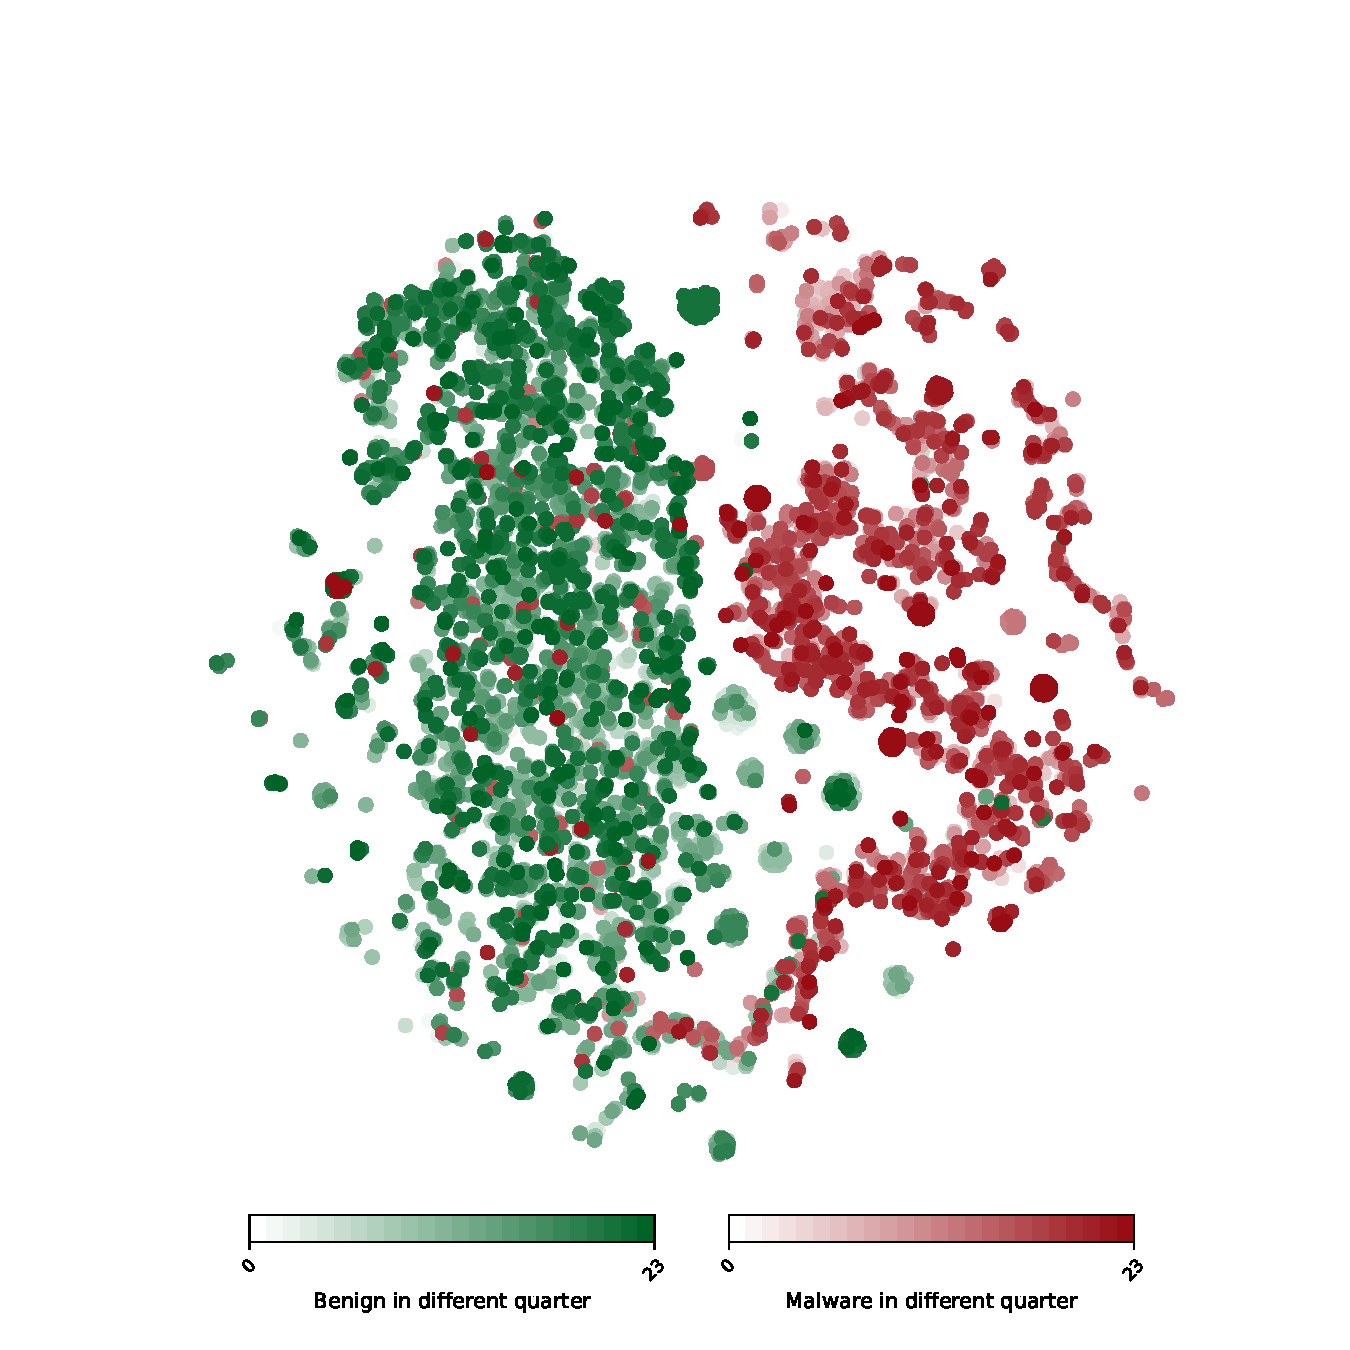
\includegraphics[width=3cm,height=3.5cm]{Graph/Motivation/tsne-APIGraph-v3}
%		\caption{APIGraph}
%		\label{fig::APIGraph PTXY concept drift dataset}
%	\end{subfigure}
%	\hspace{0.5cm}
%	\begin{subfigure}{0.20\textwidth}
%		\centering
%		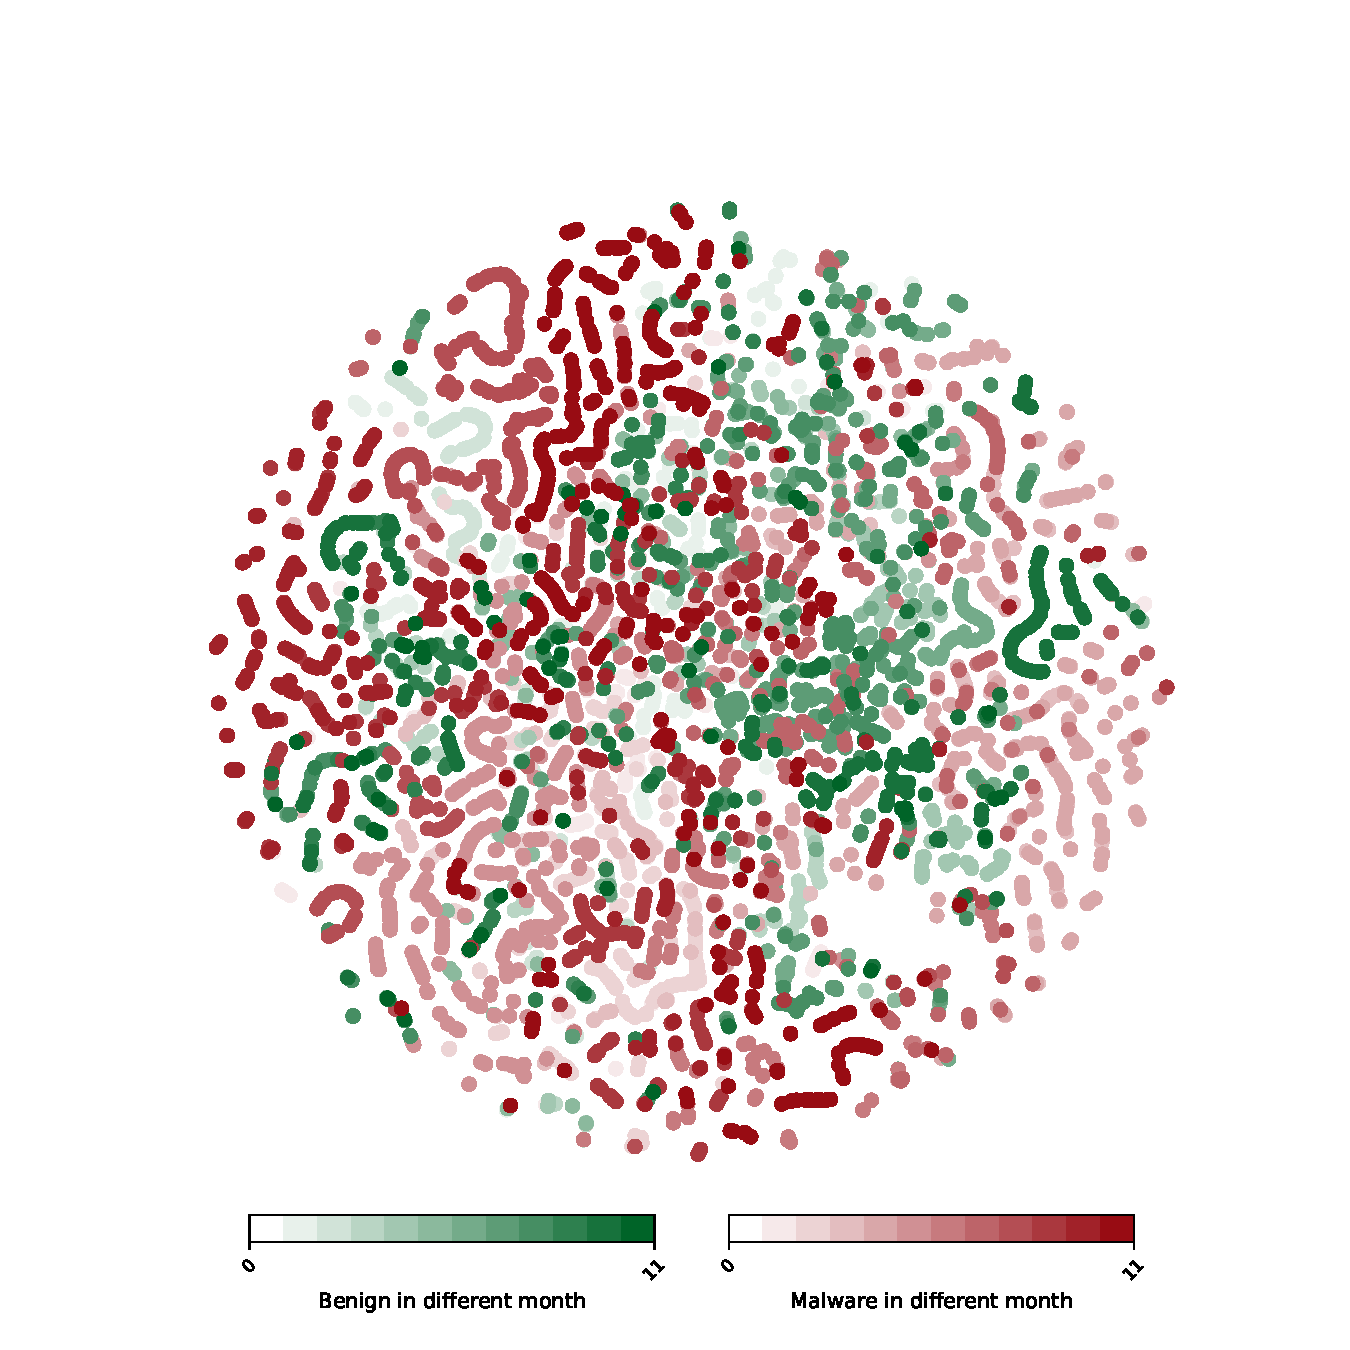
\includegraphics[width=3cm,height=3.5cm]{Graph/Motivation/tsne-BODMAS-v3}
%		\caption{BODMAS}
%		\label{fig::BODMAS PTXY concept drift dataset}
%	\end{subfigure}
%	\caption{T-SNE visualization of $P_{t}(\mathcal{X}|\mathcal{Y})$ concept drift in Android and Windows Malware Datasets}
%	\label{fig:PTXY concept drift in Malware Datasets}
%\end{figure}
%Malware samples may mimic benign characteristics or exhibit distinct malicious features, resulting in continuous changes in the feature distribution, as shown in Figure~\ref{fig:PTXY concept drift in Malware Datasets}.
%Consequently, at the time $t+1$, predicting the shift in $P_{t+1}(\mathcal{X}|\mathcal{Y})$ relative to $P_{t}\mathcal{X}|\mathcal{Y})$ becomes increasingly challenging.
%
%\noindent \textbf{(2) $P_{t}(\mathcal{Y})$ Concept Drift:} 
%Figure~\ref{fig:Attack Motivation-1} illustrates the quarterly distribution of the top 10 categories. 
%Given the significantly higher proportion of benign samples than malware samples, the largest category consists of benign samples, while the remaining nine are malicious families.
%Notably, the distribution shown reflects the label distribution of concept drift samples.
%\begin{figure}[htbp]
%	\centering
%	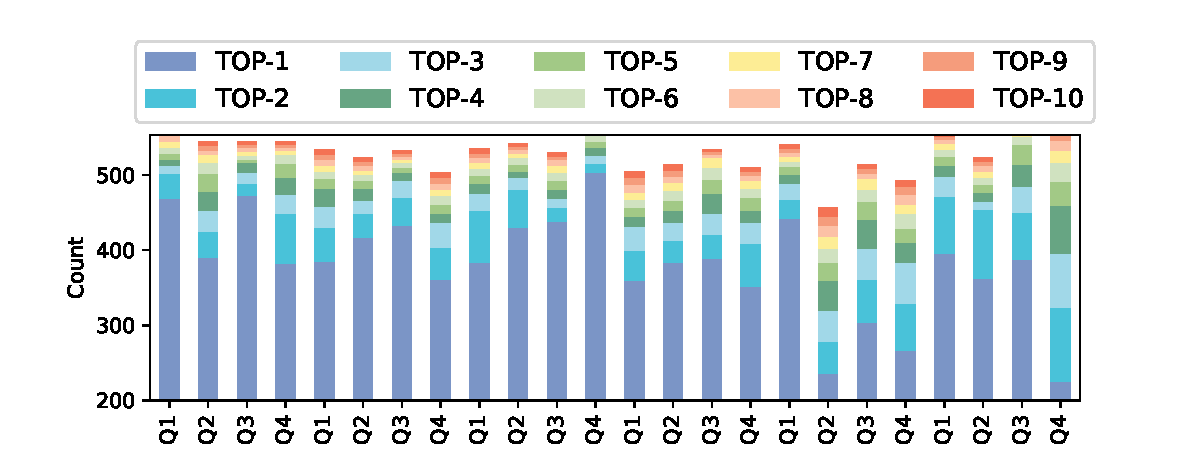
\includegraphics[width=\linewidth,keepaspectratio]{Graph/Evaluation/Figure2.pdf}
%	\caption{$P_{t}(\mathcal{Y})$ Concept Drift during 6 years}
%	\label{fig:Attack Motivation-1}
%\end{figure}
%In practice, the sample selection process is automated, leaving the model owner without access to any information about the distribution of concept drift samples before labeling.
%As a result, filtering poisoned samples becomes significantly more challenging.

\subsection{Shapley Additive Explanations}
\label{Sec: Shapley Additive Explanations}
Recent advances in explainable machine learning have introduced various methods for interpreting the predictions of complex models~\cite{ali2023explainable}.
SHapley Additive exPlanations~\cite{lundberg2017unified} adopt the Shapley value concept from cooperative game theory to assign each feature a contribution score based on its influence on the model's output.
The SHAP framework has been shown to subsume several earlier model explanation techniques~\cite{2021-Usenix-Poisoning-Attack-Explanation-guided-Backdoor}, including LIME~\cite{ribeiro2016should} and Integrated Gradients~\cite{sundararajan2017axiomatic}. 
These model explanation frameworks help determine the importance of each feature value in the model's prediction.
\begin{equation}
	\begin{aligned}
			g(\bm{\mathrm{x}}) = \phi_{0} + \sum_{j=1}^{M} \phi_{j} x_{j}
		\end{aligned}
	\label{SHAP}
\end{equation}
Explanation frameworks construct a surrogate linear model using the input feature vectors and output predictions, leveraging its coefficients to estimate feature importance and direction, as shown in Equation~\ref{SHAP}.
$\bm{\mathrm{x}}$ is the sample, $x_{j}$ is the $j^{th}$ feature for sample $\bm{\mathrm{x}}$, and $\phi_{j}$ is the contribution of feature $x_{j}$ to the model’s prediction.
The SHAP framework stands out by providing theoretical guarantees for calculating feature contributions in a model-agnostic manner.
Recent studies have extended model prediction explanations to include explanations of prediction uncertainty~\cite{NEURIPS2023_16e4be78}.
Motivated by this, we incorporate SHAP-based uncertainty attribution into the design of our poisoning attack against concept drift adaptation methods.

\subsection{Concept Drift Dataset Settings}
\label{Sec: Concept Drift Dataset Settings}
Concept drift datasets have significantly advanced machine learning research due to their rich temporal attribute information.
However, collecting natural concept drift datasets poses challenges, as it incurs significant costs and demands accurate temporal attributes.
Therefore, synthetic datasets are often constructed for experimental evaluation in existing studies, in addition to real-world datasets.

\subsubsection{Synthetic Dataset Construction}
\label{Sec: Synthetic Concept Drift Dataset Construction}
In this experimental evaluation, we constructed synthetic concept drift datasets using a publicly available spam email dataset (SPAM-Email~\cite{2010-Spam-Emali-dataset}) and the MNIST image dataset~\cite{2017-MINIST-dataset}.

\begin{itemize}[leftmargin=*]
	\item[$\bullet$] \textbf{MNIST:} 
	We processed the MNIST handwritten digit dataset to simulate the concept drift phenomenon. 
	Specifically, we selected two clusters of digits, close in the feature space, to represent two classes: digits 3, 5, and 8 (labeled as 0) and digits 4, 7, and 9 (labeled as 1).
	Each digit is treated as a subclass, with new subclasses gradually introduced based on feature similarity to simulate gradual concept drift.
	We randomly selected 30\% of the data from digits 3 and 4 for the initial training set.
	The subsequent five cycles were used as testing periods, each selecting a portion of the unused data as the testing data.
	
	\item[$\bullet$] \textbf{SPAM-Email:} 
	Similar to the concept drift construction in the MNIST dataset, we conducted an in-depth analysis of the original SPAM dataset.
	Using sklearn's k-means algorithm with default parameters, we subdivided legitimate and spam emails into 12 clusters, each representing a distinct subclass.
	Based on this, we designed a concept drift partitioning scheme with nine cycles, each containing 1,036 samples and an approximate 3:1 ratio of legitimate to spam emails.
	To simulate concept drift, we introduced a new subclass of legitimate and spam emails in each cycle while ensuring data from the same subclass appeared in consecutive cycles to reflect emerging trends.
	The first cycle served as the training data, containing one subclass for legitimate emails and one for spam. In subsequent testing cycles, new subclasses were introduced, and the proportions of existing subclasses were adjusted, ensuring at least four subclasses were present in each cycle.
	This approach enabled a smooth evolution of the data distribution over time while ensuring orderly family replacement.
\end{itemize}

\subsection{Training and Testing Data Splits}
\label{Sec: Training and Testing Data Splits}
Most training and testing data partitions are static, with the model trained on the training dataset and evaluated on a fixed testing data.
However, testing data in concept drift scenarios are dynamic and continuously evolving.
Both the distribution and size of the testing data change as time progresses.

\begin{itemize}[leftmargin=*]
	\item[$\bullet$] \textbf{APIGraph:} The APIGraph~\cite{2020-CCS-APIGraph} dataset is trained on data from 2012, with concept drift testing conducted on data from 2013 to 2018, where the data for each year is incrementally released monthly.
	The ratio of legitimate to malicious software for each year is roughly maintained at 9:1, simulating the real-world scenario where legitimate samples significantly outnumber malicious ones.
	Detailed data partitioning is provided in Table~\ref{tab: APIGraph Dataset}.
	
	\item[$\bullet$] \textbf{Androzoo:} The Androzoo\cite{2016-Androzoo} dataset is trained on data from 2017, with concept drift testing conducted on data from 2018 to 2022, where the data for each year is incrementally released monthly.
	The experimental settings for the other datasets are similar to those used for the APIGraph~\cite{2020-CCS-APIGraph} dataset.
	Detailed data partitioning is provided in Table~\ref{tab: Androzoo Dataset}.
	
	\begin{table}[h!]
		\caption{Android Concept Drift Dataset (Androzoo)}
		\label{tab: Androzoo Dataset}
		\setlength{\tabcolsep}{5.8pt}
		\begin{center}
			\scalebox{1.0}{
				\begin{tabular}{cccc}
					\toprule
					\textbf{Year}&\textbf{Malware}&\textbf{Benign}&\textbf{Malware Family}\\
					\midrule
					Train-2017 & 2,108 & 18,972 & 192\\ 
					%				\specialrule{0.05em}{1pt}{1pt}
					Test-2018 (Cycle 1) & 4,625 & 41,625 & 363\\
					%				\specialrule{0.05em}{1pt}{1pt}
					Test-2019 (Cycle 2)& 8,612 & 77,508 & 354\\ 
					%				\specialrule{0.05em}{1pt}{1pt}
					Test-2020 (Cycle 3)& 3,512 & 31,608 & 283\\
					%				\specialrule{0.05em}{1pt}{1pt}
					Test-2021 (Cycle 4)& 4,903 & 44,127 & 256\\
					%				\specialrule{0.05em}{1pt}{1pt}
					Test-2022 (Cycle 5)& 2,814 & 25,326 & 136\\
					\specialrule{0.05em}{1pt}{1pt}
					Total & 26,574 & 239,166 & 1,584\\
					\bottomrule
			\end{tabular}}
		\end{center}
	\end{table}
	
	
	\item[$\bullet$] \textbf{BODMAS:}
	The BODMAS~\cite{2021-PE-malware-dataset} dataset comprises 57,293 malware samples and 77,142 benign samples.
	The malware samples were randomly selected monthly from a security company's internal malware database, and data collection lasted from August 29, 2019, to September 30, 2020.
%	\begin{table}[t]
%		\begin{center}
%			\caption{Windows Malware Concept Drift Dataset} %标题
%			\label{tab: BODMAS Dataset} %表标签
%			\renewcommand{\arraystretch}{0.8}  % 调整该表格的行距
%			\begin{tabular}{cccc} %c的个数表示表的列数
%				\toprule
%				\textbf{Year} & \textbf{Malware} & \textbf{Benign} & \textbf{Malware Family}\\
%				\midrule
%				Train(before 10/19) & 4741 & 17655 & 330\\ 
%				Test-10/19 & 4549 & 3925 & 236 \\
%				Test-11/19 & 2494 & 3718 & 146 \\ 
%				Test-12/19 & 4039 & 6120 & 147 \\ 
%				Test-01/20 & 4510 & 5926 & 183 \\ 
%				Test-02/20 & 4269 & 3703 & 166 \\ 
%				Test-03/20 & 4990 & 3577 & 192 \\ 
%				Test-04/20 & 4640 & 5201 & 162 \\
%				Test-05/20 & 5449 & 6121 & 180 \\
%				Test-06/20 & 4217 & 8182 & 111 \\
%				Test-07/20 & 4995 & 6392 & 144 \\
%				Test-08/20 & 3823 & 2514 & 125 \\
%				Test-09/20 & 4577 & 4198 & 152\\
%				\midrule
%				\textbf{Total} & \textbf{57293} & \textbf{77142} & \textbf{2274} \\
%				\bottomrule
%			\end{tabular}
%		\end{center}
%	\end{table}
	
	\begin{table}[h!]
		\caption{Windows Malware Concept Drift Dataset}
		\label{tab: BODMAS Dataset}
		\setlength{\tabcolsep}{5.8pt}
		\begin{center}
			\scalebox{1.0}{
				\begin{tabular}{cccc}
					\toprule
					\textbf{Year}&\textbf{Malware}&\textbf{Benign} &\textbf{Malware Family} \\
					\midrule
					Train(before 10/19) & 4,741 & 17,655 & 330\\  
					Test-10/19 (Cycle 1) & 4,549 & 3,925 & 236 \\
					Test-11/19 (Cycle 2) & 2,494 & 3,718 & 146 \\
					Test-12/19 (Cycle 3) & 4,039 & 6,120 & 147 \\
					Test-01/20 (Cycle 4) & 4,510 & 5,926 & 183 \\ 
					Test-02/20 (Cycle 5) & 4,269 & 3,703 & 166 \\
					Test-03/20 (Cycle 6) & 4,990 & 3,577 & 192 \\ 
					Test-04/20 (Cycle 7) & 4,640 & 5,201 & 162 \\ 
					Test-05/20 (Cycle 8) & 5,449 & 6,121 & 180 \\ 
					Test-06/20 (Cycle 9) & 4,217 & 8,182 & 111 \\ 
					Test-07/20 (Cycle 10) & 4,995 & 6,392 & 144 \\ 
					Test-08/20 (Cycle 11) & 3,823 & 2,514 & 125 \\
					Test-09/20 (Cycle 12) & 4,577 & 4,198 & 152 \\
					\specialrule{0.05em}{1pt}{1pt}
					\textbf{Total} & \textbf{57,293} & \textbf{77,142} & \textbf{2,274} \\
					\bottomrule
			\end{tabular}}
		\end{center}
	\end{table}
	
	The data collected before October 2019 is used as the initial training data, while the data collected afterward serves as the concept drift testing data, as shown in Table~\ref{tab: BODMAS Dataset}.
	The testing data is evaluated every month.
	
	\item[$\bullet$] \textbf{SPAM-Email:}
	The dataset contains spam and legitimate messages, with a moderate spam ratio of approximately 25\%.
	It includes 9,324 instances and 500 features.
	The initial training data consists of 771 legitimate emails and 265 spam emails.
	Subsequently, 265 new spam emails and 771 legitimate emails are introduced in each of the 8 concept drift testing cycles.
%	\begin{table}[htbp]
%		\begin{center}
%			\caption{Synthetic Concept Drift Dataset for SPAM-Email} %标题
%			\label{tab: Synthetic Concept Drift Dataset for SPAM-Email} %表标签
%			\renewcommand{\arraystretch}{0.8}  % 调整该表格的行距
%			\begin{tabular}{ccc} %c的个数表示表的列数
%				\toprule
%				\textbf{miner} & \textbf{Spam} & \textbf{Legitimate} \\
%				\midrule
%				Train & 265 & 771 \\ 
%				Test-1 & 265 & 771 \\ 
%				Test-2 & 265 & 771 \\ 
%				Test-3 & 265 & 771 \\ 
%				Test-4 & 265 & 771 \\ 
%				Test-5 & 265 & 771 \\ 
%				Test-6 & 265 & 771 \\
%				Test-7 & 265 & 771 \\
%				Test-8 & 265 & 771 \\
%				\midrule
%				\textbf{Total} & \textbf{2387} & \textbf{6937} \\
%				\bottomrule
%			\end{tabular}
%		\end{center}
%	\end{table}
	
		\begin{table}[h!]
		\caption{Synthetic Concept Drift Dataset for SPAM-Email}
		\label{tab: Synthetic Concept Drift Dataset for SPAM-Email}
		\setlength{\tabcolsep}{5.8pt}
		\begin{center}
			\scalebox{1.0}{
				\begin{tabular}{ccc}
					\toprule
					\textbf{miner} & \textbf{Spam} & \textbf{Legitimate} \\
					\midrule
					Train & 265 & 771 \\ 
					Test-1 (Cycle 1) & 265 & 771 \\ 
					Test-2 (Cycle 2) & 265 & 771 \\ 
					Test-3 (Cycle 3) & 265 & 771 \\ 
					Test-4 (Cycle 4) & 265 & 771 \\ 
					Test-5 (Cycle 5) & 265 & 771 \\ 
					Test-6 (Cycle 6) & 265 & 771 \\
					Test-7 (Cycle 7) & 265 & 771 \\
					Test-8 (Cycle 8) & 265 & 771 \\
					\specialrule{0.05em}{1pt}{1pt}
					\textbf{Total} & \textbf{2,387} & \textbf{6,937} \\
					\bottomrule
			\end{tabular}}
		\end{center}
	\end{table}
	
	\item[$\bullet$] \textbf{MNIST:}
	The MNIST dataset contains handwritten digits. 
	3,591 samples were used for training, and 31,860 samples were distributed across 5 concept drift testing cycles.
%	\begin{table}[htbp]
%		\begin{center}
%			\caption{Synthetic Concept Drift Dataset for MNIST} %标题
%			\label{tab: Synthetic Concept Drift Dataset for MNIST} %表标签
%			\renewcommand{\arraystretch}{0.8}  % 调整该表格的行距
%			\begin{tabular}{ccc} %c的个数表示表的列数
%				\toprule
%				\textbf{Year} & \textbf{Label-1} & \textbf{Label-0} \\
%				\midrule
%				Train & 1752 & 1839 \\ 
%				Test-1 & 1752 & 2923 \\ 
%				Test-2 & 2421 & 2852 \\ 
%				Test-3 & 2463 & 2867 \\ 
%				Test-4 & 2734 & 2603 \\ 
%				Test-5 & 6930 & 4315 \\ 
%				\midrule
%				\textbf{Total} & \textbf{18052} & \textbf{17399} \\
%				\bottomrule
%			\end{tabular}
%		\end{center}
%	\end{table}

	\begin{table}[h!]
	\caption{Synthetic Concept Drift Dataset for MNIST}
	\label{tab: Synthetic Concept Drift Dataset for MNIST}
	\setlength{\tabcolsep}{5.8pt}
	\begin{center}
		\scalebox{1.0}{
			\begin{tabular}{ccc}
				\toprule
				\textbf{Year} & \textbf{Label-1} & \textbf{Label-0} \\
				\midrule
				Train & 1,752 & 1,839 \\ 
				Test-1 (Cycle 1) & 1,752 & 2,923 \\ 
				Test-2 (Cycle 2) & 2,421 & 2,852 \\ 
				Test-3 (Cycle 3) & 2,463 & 2,867 \\ 
				Test-4 (Cycle 4) & 2,734 & 2,603 \\ 
				Test-5 (Cycle 5) & 6,930 & 4,315 \\
				\specialrule{0.05em}{1pt}{1pt}
				\textbf{Total} & \textbf{18,052} & \textbf{17,399} \\
				\bottomrule
		\end{tabular}}
	\end{center}
\end{table}

\end{itemize}


%\subsection{Victim Model Settings}
%\label{Sec: Victim Model Settings}
%We adopt commonly used or well-performing architectures from prior research~\cite{2023-Usenix-chenyizhen,2022-SP-Trancending,2021-Usenix-CDAE} in machine learning tasks for the victim model setup. 
%All experiments are conducted on a Windows 11 system with 96GB memory, one Intel® Core™ i7-14700K 3.4GHz CPU, and an NVIDIA GeForce RTX 4080 SUPER (16GB).
%We present the model parameters optimized for respective classification tasks.
%\begin{table}[htbp]
%	\centering
%	\small
%	\caption{Parameters Setting of CDA-AL}
%	\label{tab: Parameter setting of active learning method}
%	%\renewcommand{\arraystretch}{1.2} % 调整单元格高度
%	\begin{tabular}{c|c c}
%		\hline
%		\textbf{Parameter} & \textbf{APIGraph} & \textbf{MNIST}\\ \hline
%		Optimizer  & SGD & ADAM\\ 
%		LR & 0.003 & 0.0004\\ 
%		Batch size & 1024 & 64\\ 
%		Loss & hi-dist-xent & triplet-mse\\ 
%		LR decay & 0.05 & - \\ 
%		Decay epochs & 10,500,10 & -\\
%		Learning epochs & 50 & 5\\ 
%		\hline
%		\textbf{Parameter} & \textbf{BODMAS} & \textbf{SPAM-Email} \\
%		\hline
%		Optimizer & AdamW & AdamW \\ 
%		LR & 0.0004 & 0.0004 \\ 
%		Batch size & 64 & 64 \\ 
%		Loss & BCE & BCE \\ 
%		LR decay & - & - \\ 
%		Decay epochs & - & - \\
%		Learning epochs & 50 & 5\\ 
%	\end{tabular}
%\end{table}
%Table~\ref{tab: Parameter setting of active learning method} summarizes the parameter settings for experiments conducted on four datasets: APIGraph~\cite{2020-CCS-APIGraph}, MNIST~\cite{2017-MINIST-dataset}, BODMAS~\cite{2021-PE-malware-dataset}, and SPAM-Email~\cite{2010-Spam-Emali-dataset}.
%APIGraph: SGD optimizer with a learning rate (LR) of 0.003, batch size 1024, and hi-dist-xent loss function.
%The learning rate decay was set to 0.05 and applied at epochs 10, 500, and 10.
%The model was trained for 50 epochs.
%MNIST: Adam optimizer with an LR of 0.0004, batch size 64, and triplet-my loss function. 
%No learning rate decay was applied, and the model was trained for five epochs.
%BODMAS and SPAM-Email: AdamW optimizer with an LR of 0.0004, batch size 64, and binary cross-entropy (BCE) loss function.
%No learning rate decay was applied.
%The model was trained for 50 epochs on BODMAS and five epochs on SPAM-Email.

	
\begin{figure*}[ht]
	%\setlength{\belowcaptionskip}{-1.5em} % 控制图片标题与后续文本之间的间距
	\centering
	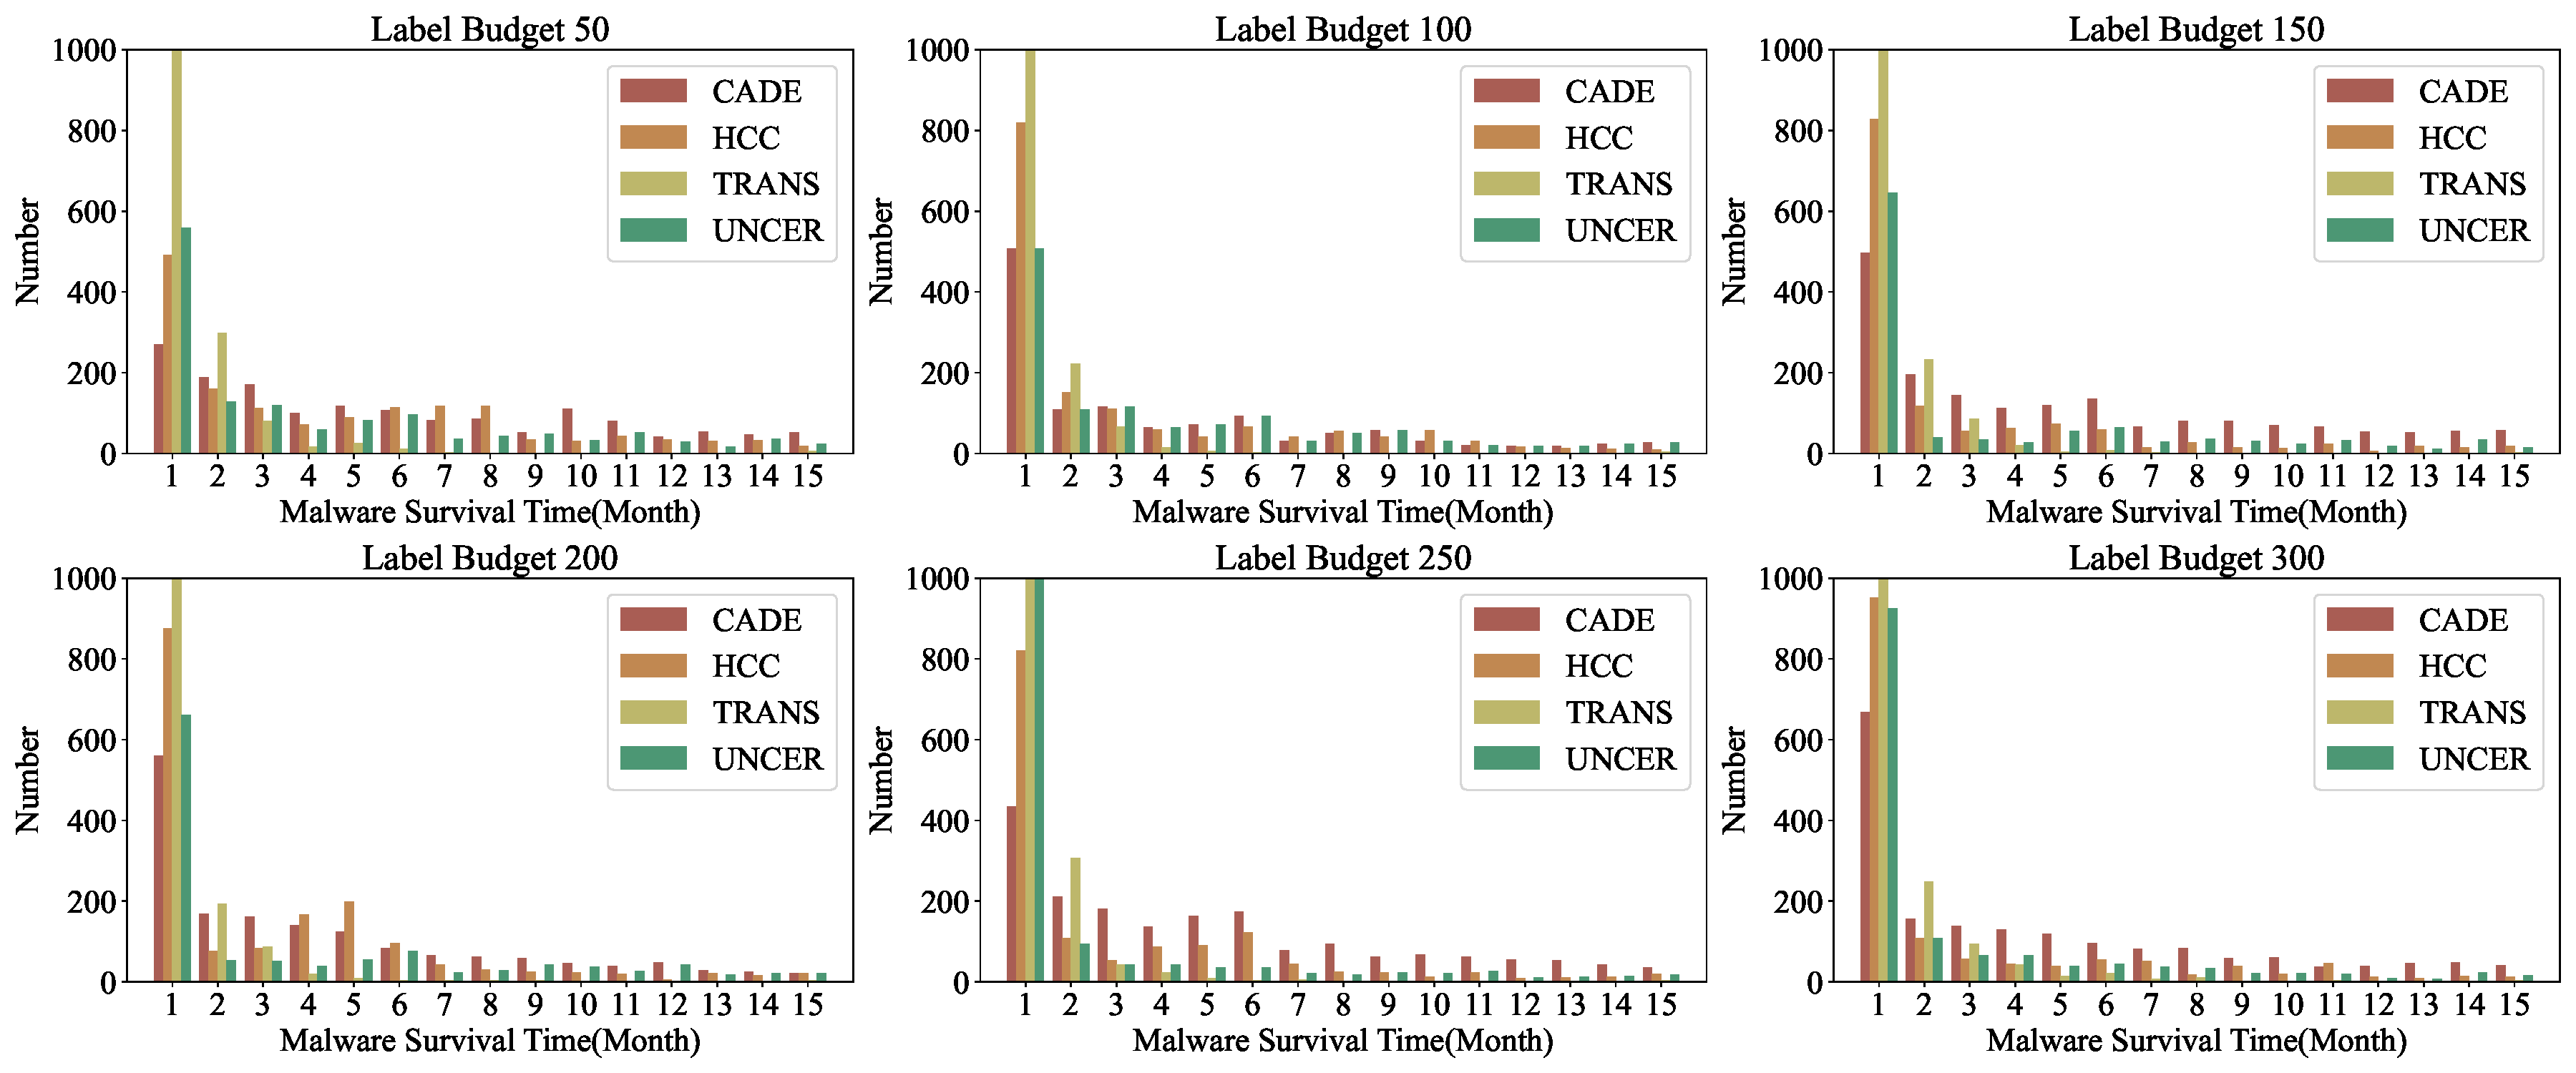
\includegraphics[width=\linewidth,keepaspectratio]{Graph/Appendix/Original_threat_life_cycle_all_budget_0901.pdf}
	\caption{Original misclassification time of attack targets}
	\label{fig: Original survival time of all budget}
\end{figure*}
%\subsection{Concept Drift Adaptation Strategies}
%\label{Sec: Concept Drift Adaptation Strategies}
%
%
%%\textbf{Model Uncertainty.} The core idea of uncertainty measurement~\cite{2023-survey-uncertainty-in-deep-neural-networks} is to detect concept drift based on the output layer of the target model. 
%%The model gives priority to selecting the samples with high uncertainty of the current model for labeling. 
%%A common uncertainty measurement for a neural network is to use one minus the max softmax output of the network.
%
%\noindent \textbf{ (1) Encoder Space Distance (CADE):} CADE~\cite{2021-Usenix-CDAE} trains an encoder through existing labeled data for learning a compressed representation (dimension reduction) of a given input distribution. 
%Then, the newly obtained test samples can be provided to the encoder to obtain the encoder's spatial features. 
%Finally, the distance function can effectively identify concept drift samples far from the existing training dataset.
%
%\noindent \textbf{(2) Credibility and Confidence (TRANS):} Transcending~\cite{2022-SP-Trancending} introduced the thery of conformal prediction~\cite{2005-high-cite-Algorithmic-learning-in-a-random-world} (credibility and confidence) into the field of concept drift adaptation. 
%Given a new test sample, Transcending first computes the non-conformity score of the sample. 
%Then, it computes credibility as the percentage of samples in the calibration set that have higher non-conformity scores than the test sample. 
%Finally, it computes confidence as one minus the credibility of the opposite label. 
%A lower credibility score or a lower confidence score means the test sample is more likely to have drifted.

%\noindent \textbf{(3) Hierarchical Contrastive Loss (HCL):} The method proposed by Chen et al.~\cite{2023-Usenix-chenyizhen} is currently the best-performing strategy in Android malware concept drift adaptation methods. 
%The model consists of two modules. 
%The first module is an encoder and the second module acts as the classifier. 
%In terms of loss function settings, to ensure that the model is robust to concept drift, the training loss of the model is set to the sum of hierarchical contrast loss and classification loss.
%The advantage of this strategy is its provision of finer-grained encoder rules and utilization of similar features among malware families, ultimately enhancing concept drift adaptation performance.


% 2025-Usenix-投稿拒绝
%\section{Original Survival Time of All Label Budget}
%\label{Sec: Original Survival Time of All Label Budget}
%
%\noindent We have analyzed the survival time of new malware under different label budget settings and various concept drift adaptation strategies, as shown in Figure \ref{fig: Original survival time of all budget}. 
%We can observe that the survival time of new malware exhibits a consistent trend, regardless of the label settings and concept drift adaptation strategies.
%Most new malware can survive for 1-5 months under concept drift adaptation strategies, a small portion can survive for more than 5 months, while the survival time of most old malware samples is 0.
%Moreover, most concept drift adaptation strategies face the situation that some new malware survives for more than one year under sufficient label budget (300 samples).
%This phenomenon fully indicates that there is still room for improvement in the performance of the current concept drift adaptation strategies.
%Due to the uneven distribution of survival times for new malware samples under the TRANS concept drift adaptation strategy, the number of samples with survival times of 0-2 months exceeds five times that of samples in other time intervals. 
%Therefore, for the sake of convenient presentation, we have truncated the bar chart representing the 0-2 months survival time samples in the TRANS statistics, while preserving the relative proportions of the overall sample volumes.
%\begin{figure*}[ht!]
%	%\setlength{\belowcaptionskip}{-1em} % 控制图片标题与后续文本之间的间距
%	\centering
%	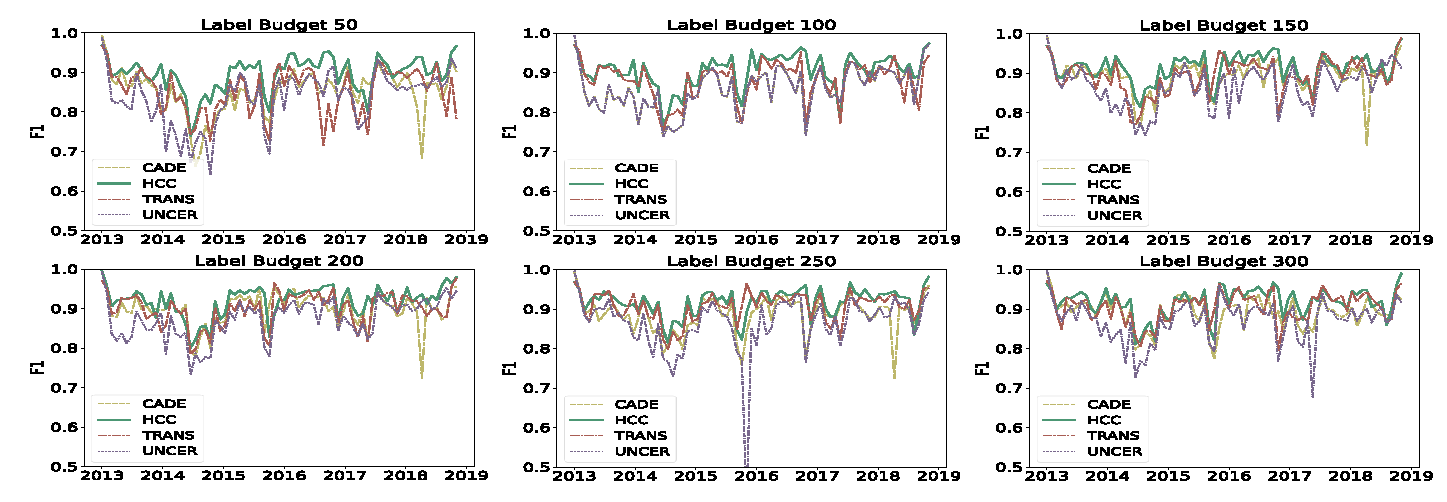
\includegraphics[width=\linewidth,keepaspectratio]{Graph/Appendix/base_performance_allbudget_0830.pdf}
%	\caption{Concept drift adaptation baseline}
%	\label{fig: CDA-AL Baseline}
%\end{figure*}

% \label{sec: Testing of attack overhead in problem space}
% %\vspace{-1em}
% \begin{table}[H]
	% \centering
	% \caption{APK obfuscation time}
	% %\renewcommand{\arraystretch}{0.8}  % 调整该表格的行距
	% \label{tab: APK obfuscation time}
	% \begin{tabular}{c|c|c|c}
		% \toprule
		% \textbf{APK} & \textbf{Size(MB)} & \textbf{Category} & \textbf{Obfuscation} \\
		% \midrule
		% \textbf{JD} & 97.59 & shopping & 54.95s \\
		% \textbf{Taobao} & 57.03 & shopping & 78.98s \\
		% \textbf{Little Red Book} & 162.99 & social & 178.68s \\
		% \textbf{Google} & 315.67 & tool & 93.32s \\
		% \textbf{Wang VPN} & 45.51 & tool & 14.91s \\
		% \textbf{WeChat} & 264.04 & communication & 136.76s \\
		% \midrule
		% \textbf{Average} & 199.72 & - & 90.72s \\
		% \bottomrule
		% \end{tabular}
	% \end{table}

% 这个先不说了
% \textbf{Feature Space Inverse Mapping:} In the end, we need to show that the features corresponding to the poison samples must have corresponding Android applications in the problem space. Since an attack seed sample is an object in the problem space that meets semantic requirements, and the poison samples are single-bit flip variants of the attack seed sample in the feature space, so they also meet semantic requirements in the problem space. For feature spaces such as the APIGraph dataset and the Androzoo dataset, a single transformation means an increase or decrease in an API call or permission declaration. 

%\section{Concept Drift Adaptation Strategy Settings}
%\label{sec: Concept Drift Adaptation Strategy Settings}
%\noindent It is not enough to just enumerate the model structures and concept drift adaptation strategies. 
%What is more critical is to combine them. 
%Our combination follows the principle of optimal configuration. 
%For each target model structure, we select the corresponding concept drift adaptation strategy based on the optimal combination method in existing research methods.
%The last setting about the concept drift adaptation strategy is the initial state of the target model. 
%Our setting in this study is to train the initial data for 1 year, then conduct \pandora attack verification, and use the monthly time window to evaluate and verify the effectiveness of the attack.
%The final combination is shown in Table \ref{tab: Combination of Model Structure and CDA-Strategy}.

%\section{Concept Drift Adaptation Baseline}
%\label{sec: CDA-AL Baseline}
%\noindent We conduct baseline tests on the performance of current mainstream concept drift adaptation methods on the APIGraph~\cite{2020-CCS-APIGraph} and CDAMAL\footnote{\url{https://anonymous.4open.science/r/Denial-of-Concept-Drift-Adaptation-Contribution-343C}} datasets, and the test results are shown in the Figure \ref{fig: CDA-AL Baseline}. 
%We run all experiments on a Win11 with 96GB memory, 1 Intel (R) Core (TM)i7-14700K 3.4GHz CPU and one NVIDIA GeForce RTX 4080 SUPER (16GB). 
%\begin{comment}
%	\begin{table}[h]
%		\centering
%		\small
%		\caption{Parameter setting of active learning method}
%		\label{tab: Parameter setting of active learning method}
%		%\renewcommand{\arraystretch}{1.2} % 调整单元格高度
%		\begin{tabular}{c|c c}
%			% \hline
%			\multirow{2}{*}{Parameter} & \multicolumn{2}{c}{Method} \\ \cline{2-3} 
%			& \textbf{HCL} & \textbf{CADE}\\ \hline
%			Optimizer  & SGD & ADAM\\ 
%			LR & 0.003 & 0.0001\\ 
%			Batch size & 1024 & 32\\ 
%			Loss & hi-dist-xent & triplet-mse\\ 
%			LR decay & 0.05 & 1\\ 
%			Decay epochs & 10,500,10 & 10,500,10\\
%			Scheduler & step & cosine\\ 
%			Learning epochs & 50 & 50\\ 
%			\hline
%			Parameter & \textbf{TRANS} & \textbf{UNC} \\
%			\hline
%			Optimizer & SGD & SGD \\ 
%			LR & 0.003 & 0.003 \\ 
%			Batch size & 512 & 1024 \\ 
%			Loss & hi-dist & hi-dist-xent \\ 
%			LR decay & 0.95 & 0.95 \\ 
%			Decay epochs & 10,500,10 & 30,1000,30 \\
%			Scheduler & step & step \\ 
%			Learning epochs & 50 & 50\\ 
%		\end{tabular}
%	\end{table}
%\end{comment}
%Here, we offer a concise overview of the hyperparameter configurations. 
%We utilize the SGD optimizer for HCL, TRANS, and UNC while employing the ADAM optimizer for CADE. 
%For the loss functions, TRANS uses the Hierarchical Distance loss function, CADE uses the Triplet Mean Squared Error loss function, and HCL and UNC employe the Hierarchical Distance Cross-Entropy loss function. 
%The total number of training epochs is set to 50 for all four methods.
%More detailed hyperparameter settings are shown in Table \ref{tab: Parameter setting of active learning method}.
%In this study, we test four types of current mainstream excellent Android malware detection models~\cite{2020-CCS-APIGraph,2023-TIFS-Federated-Android-Malware-ResNet,2023-Usenix-chenyizhen}, and the obtained concept drift detection data is shown in Figure \ref{fig: CDA-AL Baseline}.
%It can be observed that the higher the label budget setting is, the better the performance of the concept drift adaptation method becomes.
%Moreover, the latest concept drift adaptation method (HCL~\cite{2023-Usenix-chenyizhen}) demonstrates performance advantage over the existing methods (TRANS~\cite{2022-SP-Trancending},CADE~\cite{2021-Usenix-CDAE},UNCER~\cite{2023-survey-uncertainty-in-deep-neural-networks}).
%We notice that the performance of existing concept drift adaptation strategies is unstable, and even the optimal HCL method has performance fluctuations.
%The instability also inspires the research on the security of concept drift adaptation strategies in our study.

%As can be seen from the figure, after 6 years, the detector's F1 score index averaged 0.73 per month, a decrease of 0.26 compared to the initial month, and the lowest point dropped to 0.32 in November 2015, with an FNR as high as 77.66\%.

% \begin{table}[h]
	% \centering
	% \small
	% \caption{Parameter setting of active learning method}
	% \label{tab: Parameter setting of active learning method}
	% %\renewcommand{\arraystretch}{1.2} % 调整单元格高度
	% \begin{tabular}{c|c c c c }
		% % \hline
		% \multirow{2}{*}{\textbf{Parameter}} & \multicolumn{4}{c}{\textbf{Method}} \\ \cline{2-5} 
		%  & \textbf{HCC} & \textbf{CADE} & \textbf{TRANS} & \textbf{UNC} \\ \hline
		% \textbf{Optimizer}  & SGD & ADAM & SGD & SGD \\ 
		% \textbf{LR} & 0.003 & 0.0001 & 0.003 & 0.003 \\ 
		% \textbf{Batch size} & 1024 & 32 & 512 & 1024 \\ 
		% \textbf{Loss} & hi-dist-xent & triplet-mse & hi-dist & hi-dist-xent \\ 
		% \textbf{LR decay} & 0.05 & 1 & 0.95 & 0.95 \\ 
		% \textbf{Decay epochs} & 10,500,10 & 10,500,10 & 10,500,10 & 30,1000,30 \\
		% \textbf{Scheduler} & step & cosine & step & step \\ 
		% \textbf{learning epochs} & 50 & 50 & 50 & 50 \\ 
		% \end{tabular}
	% \end{table}



%\section{Freeze Attack Strategy}
%\label{Sec: Attack Value Unstable}
%%\begin{figure}[h]
%%	%\setlength{\belowcaptionskip}{-1em} % 控制图片标题与后续文本之间的间距
%%	\centering    
%%	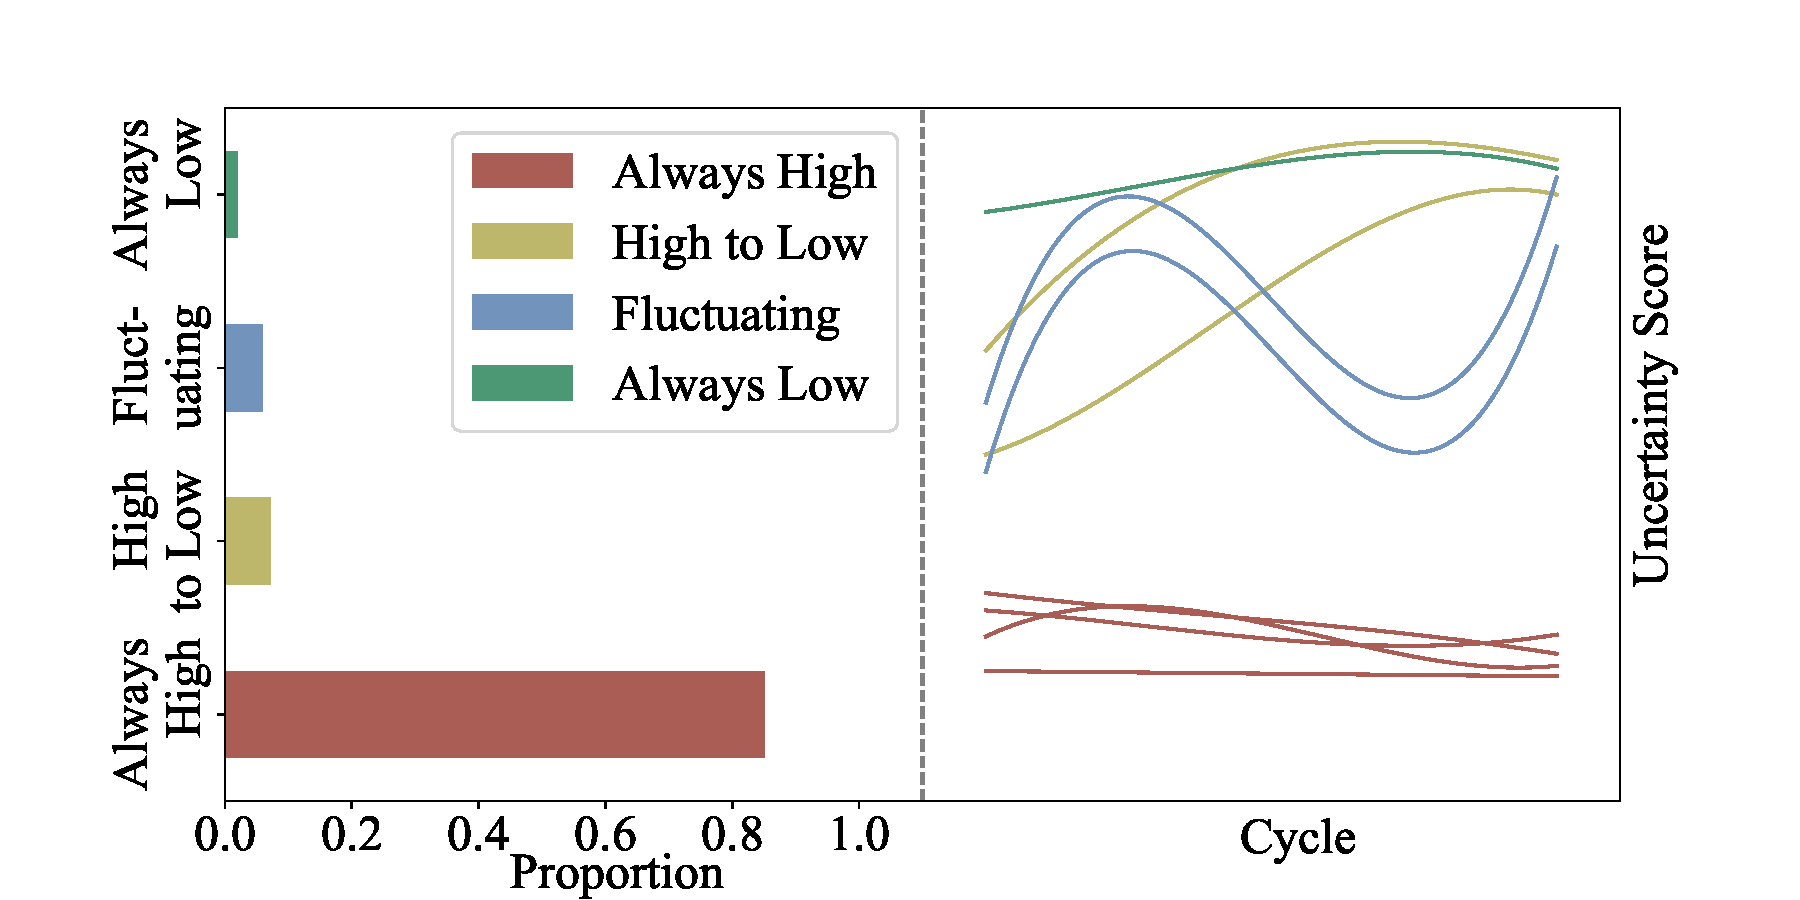
\includegraphics[width=\linewidth,keepaspectratio]{Graph/Appendix/attack_value_change_0830.pdf}       	
%%	\caption{Attack value unstable}
%%	\label{fig: Attack Value Unstable}
%%\end{figure}
%%%It is important to note that the \pandora attack framework is an automated attack framework, which needs to continuously generate poisoned samples in each model cycle.
%%Therefore, the malware attack value assessment module and the survival time prolongation module need to be integrated with each model cycle. 
%
%\noindent We observe that the attack value of new high uncertainty malware in the initial model cycle also exhibits instability in subsequent model cycles.
%%, as shown in Figure \ref{fig: Attack Value Unstable}. 
%While 85\% of the samples maintain a high attack value in the subsequent cycles, nearly 15\% of the samples experience fluctuations in their attack value.
%Specifically, the attack value of the samples may oscillate between high and low values, or it may shift from high value to low value. 
%To ensure the consistency of attack effectiveness across consecutive model cycles, we employ freeze attacks during the low attack value model cycles of new malware. 
%Freeze attack involves selecting benign poisoned seed samples with the highest uncertainty score. 
%During the poisoned sample generation phase, data augmentation based on sample replication strategies is applied to produce a batch of attack samples.


% 相关工作的这部分不放正文了,信息量太少,都是前面说过的东西
% \textbf{Concept Drift Adaptation.} Currently, researchers believe that the phenomenon of concept drift is the main reason affecting the survival time of new malware. Researchers have proposed a series of methods~\cite{2023-Usenix-chenyizhen,2022-SP-Trancending,2021-Usenix-CDAE,2017-Usenix-Transcend} to detect concept drift samples and optimize models. Furthermore, Yiling He et al.~\cite{2024-arxiv-Going-Proactive-and-Explanatory-Against-Malware-Concept-Drift} have proposed DREAM, a method that can effectively enhance the accuracy of drift detection and reduce the cost of manual analysis. Our work primarily focuses on detecting concept drift, as this phase serves as the foundation for subsequent stages. While existing research has mainly concentrated on optimizing the performance of adaptation methods for concept drift, our emphasis lies on its security.
\subsection{Model parameters}
\label{Sec: Model parameters}
APIGraph: The model was trained for 50 epochs using the SGD optimizer with a learning rate (LR) of 0.003, batch size of 1024, and hi-dist-xent loss.
A learning rate decay factor of 0.05 was applied every 10 epochs starting from epoch 10.
MNIST: The model was trained for 5 epochs with the Adam optimizer (LR = 0.0004), batch size of 64, and triplet-my loss. No learning rate decay was applied.
BODMAS and SPAM-Email: Both models used the AdamW optimizer (LR = 0.0004), batch size of 64, and binary cross-entropy (BCE) loss.
BODMAS was trained for 50 epochs and SPAM-Email for 5 epochs. No learning rate decay was applied.

\subsection{Attack Targets List}
\label{Sec: Attack Target List}
The experimental evaluation was conducted under various attack targets configurations to validate the effectiveness of the proposed method and to analyze factors influencing attack success.
The detailed information is as follows.

\begin{itemize}[leftmargin=*]
	
	\item[$\bullet$] \textbf{Single-Target Attack:} 
	We followed two principles when selecting attack targets.
	First, the attack targets must not be included in the training set.
	Second, the attack targets is misclassified during the month it appears.
	This indicates that the attack target is a newly emerging concept drift sample in the testing phase rather than a simple modification of existing samples in the training data.
	Moreover, this also prevents situations where the attack targets lack sufficient attack value.
	
	\item[$\bullet$] \textbf{Multi-Target Attack:} 
	The attack targets for multi-target attacks are composed of multiple single-attack targets that emerge simultaneously.
	The targets of APIGraph are detailed in Table~\ref{tab: Attack Target for Multi-target Attack}.
	The concept drift adaptation associated with the attack target spans five years.
	For other datasets, the multi-target attack is conducted over the entire set of attack targets.
	\begin{table}[ht!]
		\begin{center}
			\caption{Attack Target for Multi-target Attack} %标题
			\label{tab: Attack Target for Multi-target Attack} %表标签
			\renewcommand{\arraystretch}{0.8}  % 调整该表格的行距
			\begin{tabular}{ccc} %c的个数表示表的列数
				\toprule
				\textbf{Month} & \textbf{Type} & \textbf{Family} \\
				\midrule
				\multirow{6}{*}{2013-09} & \multirow{3}{*}{Non-Target} 	& ansca \\ 
				&	& cardserv \\ 
				&	& svpeng  \\ \cline{2-3}
				& \multirow{3}{*}{Target} 	& mecor  \\
				&	& smforw \\
				&	& vietsms \\
				\midrule
				\multirow{5}{*}{2014-05} & \multirow{3}{*}{Non-Target} 	& gabas \\ 
				&	& simplocker \\ 
				&	& smssend \\ \cline{2-3}
				& \multirow{2}{*}{Target} 	& mecor  \\
				&	& svpeng  \\ 
				\midrule
				\multirow{6}{*}{2014-06} & \multirow{4}{*}{Non-Target} 	& chyapo \\ 
				&	& pletor \\
				&	& spyware \\
				&   & tebak   \\ \cline{2-3}
				& \multirow{2}{*}{Target} 	& mecor \\
				&   & adflex  \\
				\midrule
				\multirow{5}{*}{2014-09} & \multirow{3}{*}{Non-Target} 	& fobus \\ 
				&	& gamecheater \\
				&   & ransomware  \\ \cline{2-3}
				& \multirow{2}{*}{Target} 	& mecor \\
				&   & spyware  \\
				\midrule
				\multirow{5}{*}{2014-10} & \multirow{3}{*}{Non-Target} 	& fakebank \\ 
				&	& systemmonitor \\
				&   & webapp  \\ \cline{2-3}
				& \multirow{2}{*}{Target} 	& airpush \\
				&   & mecor  \\
				\midrule
				\multirow{5}{*}{2015-05} & \multirow{3}{*}{Non-Target} 	& adflex \\ 
				&	& kalfere \\
				&   & styricka  \\ \cline{2-3}
				& \multirow{2}{*}{Target} 	& mobidash \\
				&   & vnapstore  \\
				\midrule
				\multirow{4}{*}{2016-07} & \multirow{1}{*}{Non-Target} 	& clicks \\  \cline{2-3}
				& \multirow{3}{*}{Target} 	& adflex \\
				&   & blouns  \\
				&   & mspy    \\
				\midrule
				\multirow{3}{*}{2017-01} & \multirow{1}{*}{Non-Target} 	& mobidash \\  \cline{2-3}
				& \multirow{2}{*}{Target} 	& batmob \\
				&   & kalfere  \\
				\midrule
			\end{tabular}
		\end{center}
	\end{table}
	
	%\noindent \textbf{(3) Dynamic Switching Between Different Attack Target Configurations:} 
	%The target selection rules are the same as those for the multi-target attack scenario.
	%The attack targets are detailed in Table~\ref{tab: Attack Target for Dynamic Switching}.
	%\begin{table}[htbp]
	%	\begin{center}
		%		\caption{Attack Target for Dynamic Switching} %标题
		%		\label{tab: Attack Target for Dynamic Switching} %表标签
		%		\renewcommand{\arraystretch}{0.8}  % 调整该表格的行距
		%		\begin{tabular}{cc|cc} %c的个数表示表的列数
			%			\toprule
			%			\textbf{Month} & \textbf{Family} & \textbf{Month} & \textbf{Family} \\
			%			\midrule
			%			\multirow{5}{*}{2014-09} & mecor & \multirow{5}{*}{2015-01} & airpush\\ 
			%									 & spyware &  & mobidash \\ 
			%									 & gamecheater &  & svpeng \\ 
			%									 & ransomware &  & kemoge \\ 
			%									 & fobus &  & gorpo \\ 
			%			\midrule
			%			\multirow{4}{*}{2016-07} & clicks & \multirow{4}{*}{2018-01} & itracker\\ 
			%									& adflex &  & faketoken \\ 
			%									& blouns &  & clicks \\ 
			%									& mspy &  & miner \\ 
			%			\midrule
			%		\end{tabular}
		%	\end{center}
	%\end{table}
\end{itemize}



\subsection{Attack Targets Initial Misclassification Time}
\label{Sec: Attack Target Initial Survival Time (APIGraph)}
Since the effectiveness of the \pandora is defined by prolonging the misclassification duration of the original attack targets, it is essential to test the misclassification duration of the attack targets in the absence of any attacks.
We analyzed the misclassification time of malware under different labeling budget settings and concept drift adaptation strategies, as shown in Figure~\ref{fig: Original survival time of all budget}.
Most malware is misclassified for 1-5 months under CDA-AL, while a small portion survives for over 5 months.
The \pandora aims to extend the misclassification duration of targeted samples. 
Therefore, we selected all malware samples in the testing phase with a misclassification duration of 15 months or less as attack targets.
We performed similar operations on the other three datasets to extract the original misclassification times of the attack targets.

%\section{Attack Method Details}
%\label{Sec: Attack Method Details}

%\subsection{The Alignability of Real-World Data}
%\label{Sec: Real-World Alignment with the Gray-Box Assumption}
%% 代理模型数据对齐相关分析
%The alignment degree between the data collection capabilities of the surrogate model and the victim model is a critical factor influencing the surrogate model's ability to simulate the victim model's inference behavior.
%However, we find that in concept drift adaptation systems for sensitive domains (e.g., VirusTotal), platform maintainers often utilize hash functions as sample indices to enable precise matching during the sample query process.
%Although exact matching improves the performance of concept drift adaptation, it inadvertently aids attackers in aligning data more effectively, allowing them to build more accurate surrogate models.
%This alignment, in turn, enhances the efficiency of \pandora attacks.
%% 现实世界代理模型黑盒与灰盒相关分析
%In black-box settings, attackers must construct surrogate models to estimate sample uncertainties, which increases their costs.
%Conversely, gray-box settings eliminate the need for surrogate models, significantly lowering attack expenses.
%Moreover, real-world machine learning systems~\cite{Baidu-ImageRecognition} provide confidence information (indicating sample uncertainty) to enhance user experience.
%This practice aligns with the gray-box assumption, making it more applicable to practical scenarios while further reducing the cost of \pandora attacks.
%The alignment between the data collection capabilities of the surrogate model and the victim model is a critical factor in simulating the victim model's inference behavior. 
%Specifically, in concept drift adaptation systems for sensitive domains (e.g., VirusTotal~\ref{Virustotaluploadinterface}), platform maintainers often use hash functions to index samples, enabling precise matching during the query process. 
%While this enhances adaptation performance, it also inadvertently aids attackers in aligning data more effectively, allowing them to build more accurate surrogate models and thereby increasing the efficiency of \pandora attacks.
%Moreover, real-world machine learning systems~\cite{Baidu-ImageRecognition} often provide confidence scores to enhance user experience. 
%This practice aligns with the gray-box assumption, making it highly relevant to practical scenarios and further lowering the cost of \pandora attacks.
%The alignment between the surrogate and victim models' data collection capabilities is critical in simulating the victim model's inference behaviour.
%Specifically, in concept drift adaptation systems for sensitive domains (e.g., VirusTotal~\cite{Virustotaluploadinterface}), platform maintainers often use hash functions to index samples, facilitating precise matching during the query process. While this improves adaptation performance, it also inadvertently helps attackers align data more effectively, enabling the construction of accurate surrogate models and enhancing \pandora attack efficiency.
%Moreover, real-world machine learning systems~\cite{Baidu-ImageRecognition} often provide confidence scores to improve user experience. 
%
%\noindent \textbf{In summary:} Real-world scenarios align more closely with the gray-box assumption, making \pandora attacks highly applicable in practical settings while simultaneously reducing their costs.

%\begin{table}[t]
%	\caption{Problem-Space Perturbation Operations} %标题
%%	\label{tab: List of Problem Space Perturbation Operations} %表标签
%	\centering
%	\renewcommand{\arraystretch}{0.95}  % 调整表格的行距
%	\small
%	\begin{tabular}{|>{\centering\arraybackslash}p{1.2cm}|>{\centering\arraybackslash}p{6.0cm}|}
%		\hline
%		\textbf{Dataset}                   & \textbf{Perturbation Operations} ($\alpha$) \\ \hline
%		\multirow{3}{*}{APIGraph} & Rename method names to meaningless identifiers            \\ \cline{2-2} 
%		& Modify image and other resource files     \\ \cline{2-2} 
%		&Transform complex control structures into simpler ones    \\ \hline
%		\multirow{3}{*}{BODMAS}   & Modify the system API function names                       \\ \cline{2-2} 
%		& Move variables to the header structure fields            \\ \cline{2-2} 
%		& Dynamically adjust the size of the DOS STUB space        \\ \hline
%		\multirow{3}{*}{MNIST}   & Add Gaussian noise to the image pixels                      \\ \cline{2-2} 
%		&  Perform geometric transformations, such as rotation                    \\ \cline{2-2} 
%		& Apply sharpening to enhance the edges of the image                        \\ \hline
%		\multirow{3}{*}{SPAM}     &  Remove non-essential words                       \\ \cline{2-2} 
%		&  Split long sentences into shorter ones                      \\ \cline{2-2} 
%		& Insert random symbols or additional spaces                        \\ \hline
%	\end{tabular}
%\end{table}

%\subsection{Attack Negotiation Details}
%\label{Sec: Attack Negotiation Details}
%% 攻击协商协议细节
%To further elaborate, the following details describe the attack negotiation process and its implementation.
%At time $t$, attacker $\mathcal{A}_{m}$ begins by evaluating the potential attack value of their target sample $x_{tar}^{m}$, as shown in Step-II-D (Figure~\ref{fig: Attack Negotiation}).
%This assessment is based on two key indicators: the predicted pseudo label $\overline{y}_{tar}^{m}$ of the attack target $x_{tar}^{m}$, generated by the surrogate model $S_{t}$, and the uncertainty score $u_{tar}^{m}$.
%The pseudo labels $\overline{y}_{tar}^{m}$ reflect the survival probability of the target sample $x_{tar}^{m}$ under the current model state at time $t$.
%Simultaneously, the uncertainty score $u_{tar}^{m}$ quantifies the likelihood that $x_{tar}^{m}$ will be flagged for manual analysis based on the label budget threshold $\beta$.
%Only samples with uncertainty $u_{tar}^{m}$ below the threshold $\beta$ are considered valuable for the attack.
%If a target sample $x_{tar}^{m}$ is submitted for manual analysis, the victim model will learn the ground truth label ${y}_{tar}^{m}$, thereby neutralizing the attack’s effect.
%Attack targets that are misclassified $\left( y_{tar}^{m} \ne \overline{y}_{tar}^{m} \right)$ under the current model state and are resistant to manual analysis hold attack value.
%Conversely, if a target does not meet these criteria, the attacker does not have sufficient time to execute a data poisoning attack effectively.
%As a result, such samples are either immediately detected as correct label during the testing cycle in which they appear or, following manual analysis, are added to the detection system's blacklist.
%For targets lacking attack value, the attacker withdraws from the current attack negotiation to conserve resources.
%To validate the effectiveness of the attack value evaluation module, we also conducted ablation experiments detailed in Appendix~\ref{Sec: Other Attack Influencing Factors under TPA}.
%After each attacker identifies their high-value targets $x_{tar}^{m}$, they proceed to negotiate the attack targets, as illustrated in Step-III to Step-VII (Figure~\ref{fig: Attack Negotiation}).
%Steps III to VII follow the standard Millionaire’s Protocol algorithm, which can also be replaced in practice with any more efficient cryptographic protocol providing equivalent functionality.

%\subsection{Side Effects of Problem-Space Perturbation}
%\label{Sec: Side Effects of Problem Space Perturbation}
%\begin{table}[htbp]
%	\caption{Problem-Space Perturbation Operations} %标题
%	\label{tab: List of Problem Space Perturbation Operations} %表标签
%	\centering
%	\renewcommand{\arraystretch}{0.9}  % 调整表格的行距
%	\small
%	\begin{tabular}{|c|c|}
%		\hline
%		\textbf{Dataset}                   & \textbf{Perturbation Operations} ($\alpha$) \\ \hline
%		\multirow{3}{*}{APIGraph} & Rename method names to meaningless identifiers            \\ \cline{2-2} 
%		& Modify image and other resource files     \\ \cline{2-2} 
%		&Transform complex control structures into simpler ones    \\ \hline
%		\multirow{3}{*}{BODMAS}   & Modify the system API function names                       \\ \cline{2-2} 
%		& Move variables to the header structure fields            \\ \cline{2-2} 
%		& Dynamically adjust the size of the DOS STUB space        \\ \hline
%		\multirow{3}{*}{MNIST}   & Add Gaussian noise to the image pixels                      \\ \cline{2-2} 
%		&  Perform geometric transformations, such as rotation                    \\ \cline{2-2} 
%		& Apply sharpening to enhance the edges of the image                        \\ \hline
%		\multirow{3}{*}{SPAM}     &  Remove non-essential words                       \\ \cline{2-2} 
%		&  Split long sentences into shorter ones                      \\ \cline{2-2} 
%		& Insert random symbols or additional spaces                        \\ \hline
%	\end{tabular}
%\end{table}
%%%%%%%%%%%%%%%
%As shown in Section~\ref{Sec: Poisoned Sample Generation}, under the condition of maintaining consistency in the feature space, the attacker generates poisoned samples using perturbations in the problem space. 
%For data domains such as images and text, the goal of poisoned samples is to reduce the performance of the victim model.
%Therefore, the attack is considered adequate as long as the poisoned samples maintain high uncertainty during the perturbation process in the problem space.
%
%We adopt the perturbation methods shown in Table~\ref{tab: List of Problem Space Perturbation Operations} during problem-space perturbations.
%Furthermore, after the perturbation in the problem space, the attacker utilizes a surrogate model as a discriminator to eliminate the samples with decreased uncertainty.
%For functional samples, such as Android applications, in addition to ensuring high uncertainty, the sample's functionality also needs to be preserved.
%The code's functionality is preserved using well-established code obfuscation techniques, as detailed in Table~\ref{tab: List of Problem Space Perturbation Operations}.
%The attacker will also use the surrogate model as the discriminator for poisoned samples.
%In Summary: All problem-space operations preserve the sample uncertainty of the poisoned samples.

%\section{Other Attack Influencing Factors}
%\label{Sec: Other Attack Influencing Factors under TPA}

%\noindent \textbf{Note:} While the attack value assessment reduces the number of attack targets, it significantly improves the utilization of attacker resources.
%Moreover, in sensitive domains, the benefits of successful poisoning attacks exhibit pronounced asymmetry, where the gains from a single successful attack far exceed the associated costs. Therefore, attackers do not need to prioritize the quantity of attack targets.

%\noindent \textbf{Impact of Different Feature Extraction Methods:}
%In real-world scenarios, victim models may employ diverse feature extraction methods. 
%To account for this variability, we collected Android malware data from the Androzoo platform and applied a feature extraction approach distinct from that used in the APIGraph dataset.
%We extract static features~\cite{2014-NDSS-Drebin}, such as permissions, from our self-constructed dataset to conduct attack experiments on heterogeneous features.
%We name the collected dataset as MalData.
%The dataset spans 6 years, comprising 265,740 samples and 1,584 malware families.
%The attack results are shown in Table~\ref{tab: Feature Heterogeneity}. 
%Our proposed \pandora attack can achieve effective attacks (with an ASR of over 90\%) against different feature extraction methods.
%Moreover, during the attack process, the model's performance remains stable compared to the non-attack state, with an average F1 score change of 0.015 and an average FNR change of 1.3\%.
%\begin{table}[htbp]
%	\centering
%	%\renewcommand{\arraystretch}{0.8}  % 调整表格的行距
%	\small
%	\caption{Feature heterogeneity}
%	%\renewcommand{\arraystretch}{0.8}  % 调整该表格的行距
%	\label{tab: Feature Heterogeneity}
%	\begin{tabular}{cccc}
%		\toprule
%		\textbf{Feature} & \textbf{F1} & \textbf{FNR (\%)} & \textbf{ASR (\%)}\\
%		\midrule
%		APIGraph~\cite{2020-CCS-APIGraph} & 0.90\textsubscript{-0.02}  & 14.12\textsubscript{+1.12} & \textbf{92.77} \\
%		MalData & 0.67\textsubscript{+0.01} & 44.57\textsubscript{+1.39} & \textbf{95.03} \\
%		\bottomrule
%	\end{tabular}
%	% \vspace{-0.5em}
%\end{table}

%\noindent \textbf{Impact of Poisoning Rate:}
%The attacker can adjust the proportion of poisoned samples relative to the victim model's label budget by controlling the number of generated poisoned samples.
%The label budget's poisoning rate represents the intensity of the \pandora attack.
%The higher the poisoning rate of the label budget, the greater the attacker's attack cost. 
%To effectively illustrate the impact of poisoning rate on attack effectiveness, we set the label budget poisoning rate to 100\%, 70\% and 50\%, respectively. 
%We then evaluate how different poisoning rates affect the attack result. 
%As shown in Table~\ref{tab: Poisoning Rate of Label Budget}, different poisoning rates of label budgets have different impacts on ASR. 
%The average ASR of multiple attack test sets can still reach 87.73\%.
%Furthermore, we can observe a clear trend in ASR: As the poisoning rate of label budget decreases, ASR gradually declines. 
%Specifically, the settings of 70\% and 50\% poisoning rates decrease by 3.88\% and 11.25\% in ASR, respectively.
%With a 50\% reduction in the poisoning rate, the ASR (Attack Success Rate) remains at 80\%.
%%This indicates that the importance of different concept drift samples varies significantly in determining the attack's success.
%%If attackers can analyze the contribution of individual samples to the attack's value, it may be possible to maintain a high attack success rate while significantly reducing the poisoning rate (computational cost).
%\begin{table}[htbp]
%\centering
%\renewcommand{\arraystretch}{0.8}  % 调整表格的行距
%\small
%\caption{Poisoning Rate of Label Budget}
%%\renewcommand{\arraystretch}{0.8}  % 调整该表格的行距
%\label{tab: Poisoning Rate of Label Budget}
%% \begin{tabular}{P{2.0cm}P{1.3cm}P{1.3cm}P{1.3cm}P{1.3cm}}
%	\begin{tabular}{ccccc}
%			\toprule
%			\textbf{Poisoning Rate} & \textbf{F1} & \textbf{FPR (\%)} & \textbf{FNR (\%)} & \textbf{ASR (\%)}\\
%			\midrule
%			100\% & 0.90 & 0.44 & 14.12 & \textbf{92.77} \\
%			70\%  & 0.90 & 0.43 & 14.22 & \textbf{88.89} \\
%			50\%  & 0.90 & 0.46 & 14.21 & \textbf{81.52} \\
%			
%			\bottomrule
%		\end{tabular}
%\end{table}
	
%\noindent \textbf{Impact of Search Space:} 
%In this study, we leverage the feature space of attack seed samples to reduce the computational cost associated with feature space perturbations during the generation of poisoned samples.
%Simultaneously, to gain deeper insights into the impact of feature space perturbations on attack success rates, we investigate their relationship, laying a foundation for future research on feature-space-based poisoning attacks.
%The sample feature search space refers to the entire feature space the attacker can perturb when generating poisoned samples based on the seed samples. 
%The \pandora attack forms the entire perturbation feature space after a single bit flip is performed on each poisoned seed sample.
%A single-bit flip has minimal impact on the original functionality of the sample.
%Additionally, poisoned samples are primarily derived from benign samples.
%To ensure label consistency, we only remove features (e.g., disabling permissions) from the samples rather than adding new ones, thus avoiding the introduction of potentially dangerous permissions.
%The larger the search space, the greater the probability that the attacker will find samples that meet the attack requirements.
%However, a larger search space will result in higher sample generation costs for the attacker.
%In this experimental evaluation, the search space was set to 100\% feature space, 90\% feature space, and 80\% feature space, respectively, to verify the impact of the search space size on the attack effect.
%We select the best concept drift adaptation method (HCL) as the concept drift adaptation strategy and set the label budget to 200 samples.
%The experimental evaluation results are shown in Table~\ref{tab: Search Space Influence Factor}.
%\begin{table}[htbp]
%	\centering
%	\small
%	\renewcommand{\arraystretch}{0.8}
%	\caption{Search space influence factor}
%	\label{tab: Search Space Influence Factor}
%	%\renewcommand{\arraystretch}{0.85}  % 调整该表格的行距
%	\begin{tabular}{cccc}
%			\toprule
%			\textbf{Search Space (\%)}  & \textbf{F1} & \textbf{FNR (\%)} & \textbf{ASR (\%)} \\
%			\midrule
%			100 & 0.90 & 14.12 & \textbf{92.77} \\
%			90 & 0.89 & 14.54 & \textbf{92.10} \\
%			80 & 0.87 & 19.16 & \textbf{95.93} \\
%			\bottomrule
%		\end{tabular}
%\end{table}
%According to the experimental result, we can see that the average ASR under different search space settings can reach 93.60\%. 
%The setting group with a 20\% reduction in search space can still achieve an ASR of 95.93\%.
%Furthermore, we have observed that the ASR may even increase as the search space decreases.
%The reason is that the reduction in search space primarily affects the quantity of poisoned samples but does not influence the uncertainty scores of these samples.
%Therefore, as long as the reduction in search space does not compromise the coverage of the label budget by the generated poisoned samples, its impact on the ASR can be considered negligible.
%Additionally, due to the varying impacts of different bit flips within the search space on the uncertainty scores of samples, poisoning samples generated in a smaller search space may exhibit higher uncertainty scores, ultimately achieving a higher ASR.
%Based on the above analysis, we know that when attackers cannot search the entire feature search space due to the limited attack cost, they can still carry out effective \pandora attacks.
%It should be pointed out that, similar to previous studies on malicious software perturbation~\cite{2021-Usenix-Poisoning-Attack-Explanation-guided-Backdoor,2021-CCS-Evasion-Attack-Graph-Attack}, our feature perturbation also adheres to label consistency and the integrity of sample functionality.
%We did not add malicious behaviors to benign samples; we only reduced some features and functions of a portion of benign samples, while keeping the labels consistent.
%As for malware samples, we only added some functions, and the existing malicious behaviours remained unchanged, with both consistent labels and functionality.
%\begin{figure}[h!]
%	\centering
%	% 第一个子图
%	\begin{subfigure}{0.20\textwidth}
%		\centering
%		\includegraphics[width=4cm,height=2cm]{Graph/Evaluation/IF-Poisoning-Rate-2024-12-24-9-41}
%		\caption{IF-Posiong Rate}
%		\label{fig: Influencing Factor-Posiong Rate}
%	\end{subfigure}
%	% 用于调整两个子图的间距
%	\hspace{0.5cm}
%	\begin{subfigure}{0.20\textwidth}
%		\centering
%		\includegraphics[width=4cm,height=3cm]{Graph/Evaluation/IF-CDA-Strategy}
%		\caption{IF-Search Space}
%		\label{fig: Influencing Factor-Search Space}
%	\end{subfigure}
%	\caption{Other Influencing Factors}
%	\label{fig: Other Influencing Factors}
%\end{figure}

%\subsection{Operability of Sample with High Uncertainty}
%\label{Sec: Operability of Sample with High Uncertainty}
%We observed that sample uncertainty is highly manipulable in domains with weaker semantic constraints, thereby facilitating poisoning attacks. 
%Taking text data as an example, attackers can flip labels while maintaining sample uncertainty, even without controlling the labeling process of the victim model.
%\begin{figure}[htbp]
%	\centering
%	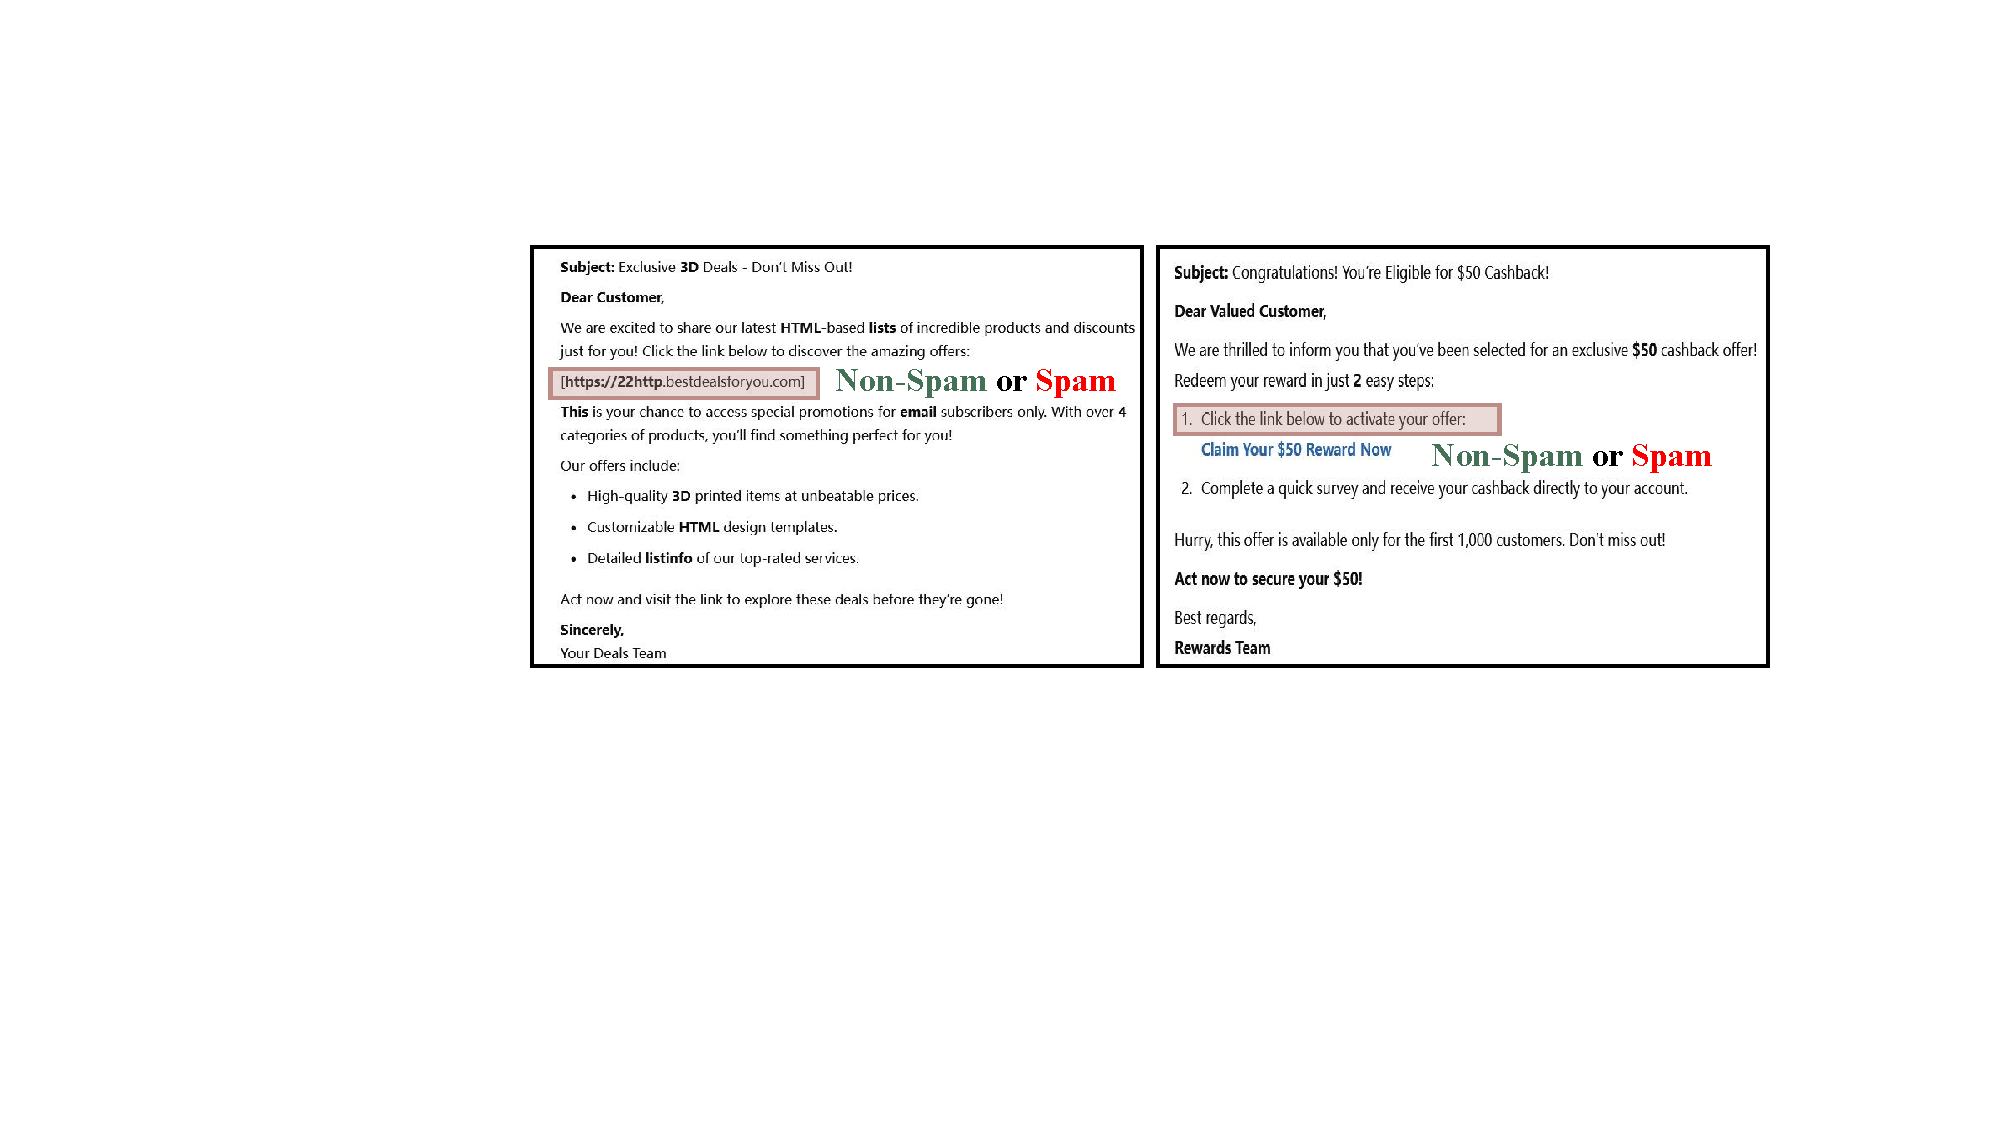
\includegraphics[keepaspectratio,height=3cm]{Graph/Evaluation/SPAM-Dynamics.pdf}
%	\caption{Uncertainty Dynamics in SPAM Email}
%	\label{fig:Uncertainty Dynamics for SPAM}
%\end{figure}
%We selected two feature vectors from spam emails in the SPAM dataset and used AIGC to generate corresponding email content.
%Whether identical feature vectors are classified as spam is not determined by the textual characteristics alone but rather by whether the embedded links are malicious.
%Attackers can exploit this by generating high-uncertainty samples with identical features but opposite labels. Such samples can significantly degrade the concept drift adaptation performance of the target model.
%For example, in spam detection, sample features are word vectors. 
%Using large language models (LLMs), attackers can generate poisoned samples with consistent features but flipped labels, adhering to the clean-label assumption through manual validation, as shown in Equation~\ref{EQ-Guided Untargeted Poisoning Attack}.
%\begin{equation}
%	\begin{aligned}
%		x_{seed}^{t+1} & = \max_{x_{p} \in D_{te}^{t}} uncer\left( x_{p+\alpha}, \theta_{t}^{*} \right)  \\
%		\text{s.t. } &
%		\begin{cases} 
%			uncer\left( x_{p+\alpha}, \theta_{t}^{*} \right)>\beta \\
%			y_{p+\alpha} \neq y_{p}
%		\end{cases}  \\
%	\end{aligned}
%	\label{EQ-Guided Untargeted Poisoning Attack}
%\end{equation}
%
%\subsection{Uncertainty Dynamics based on AIGC}
%\label{Sec: Uncertainty Dynamics based on LLM}
%With the help of generative models, attackers can perturb the uncertainty of existing samples at minimal cost.
%This is particularly significant in domains such as text, images, and videos, where the semantic meaning of labels evolves over time.
%\begin{figure}[htbp]
%	\centering
%	
\includegraphics[width=8cm,height=3cm]{Graph/Evaluation/Figure17-Bird.pdf}
%	\caption{Uncertainty Dynamics based on AIGC (Bird)}
%	\label{fig:Uncertainty Dynamics based on LLM}
%\end{figure}
%Attackers have substantial flexibility in these areas, as the real-world meanings of text and visual entities are constantly evolving.
%As shown in Figure~\ref{fig:Uncertainty Dynamics based on LLM} and Figure~\ref{fig:Uncertainty Dynamics based on LLM-Deer}, we leverage AIGC to quickly generate a series of images with gradually shifting concepts.
%As shown in Figure~\ref{fig:Uncertainty Dynamics based on LLM} and Figure~\ref{fig:Uncertainty Dynamics based on LLM-Deer}, we leverage AIGC to generate images with gradually shifting concepts quickly. 
%\begin{figure}[htbp]
%	\centering
%	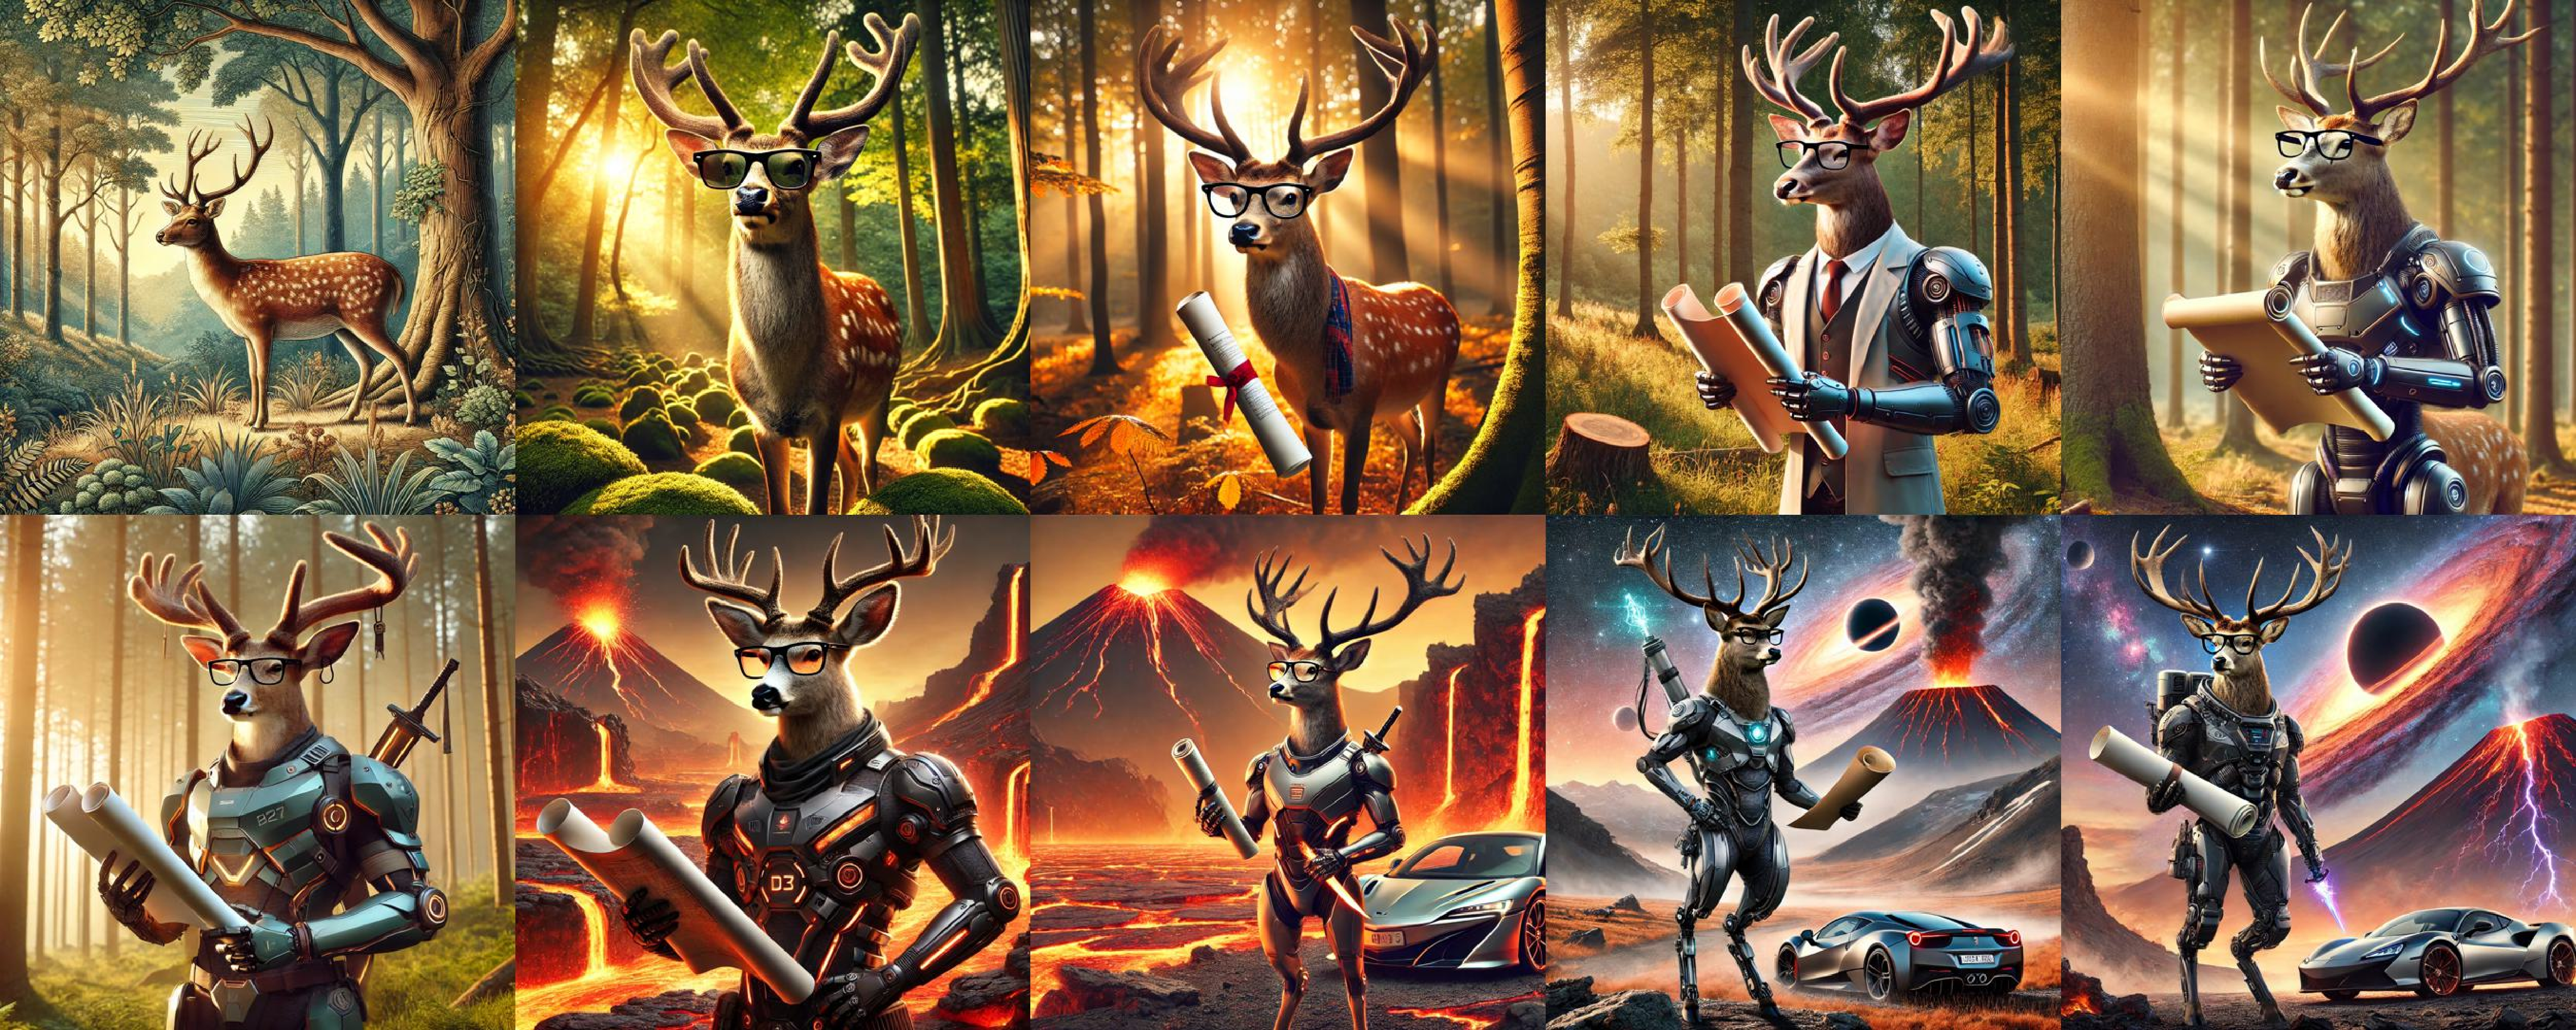
\includegraphics[width=8cm,height=3cm]{Graph/Evaluation/Figure17-deer.pdf}
%	\caption{Uncertainty Dynamics based on AIGC (Deer)}
%	\label{fig:Uncertainty Dynamics based on LLM-Deer}
%\end{figure}
%Attackers do not need to worry about label flipping, as high uncertainty is the core requirement for poisoned samples in \pandora attacks (UPA).
%Furthermore, our experiments on concept drift direction-guided untargeted attacks using the SPAM dataset (Figure~\ref{fig:Untargeted-Attack-Guided}) reveal that label flipping can even enhance the effectiveness of UPA attacks.

%\section{Attacker Cost Analysis}
%\label{Sec: Attacker Cost Analysis}
%
%\noindent The attacker’s cost structure is complicated, including manual labeling, poisoned seed sample search, and sample generation costs.
%Since the attacker’s surrogate model training phase uses pseudo labels, the active learning process has no manual labeling cost.
%The main labeling cost is used for the search of poisoned samples, which is much smaller than the annotation cost in the active learning process of the victim model, as the attacker only needs to focus on a small number of highly uncertain samples within each test cycle.
%Attackers need to pay a specific cost for the construction of poisoned samples.
%This part involves the construction of the corresponding problem space after the feature space is determined.  
%Large language models can assist attackers in constructing poisoned samples, such as poisoned images and text.
%The problem-space construction of malware samples is inherently more complex.
%However, there are also mature tools available to use~\cite{virboxprotector}.
%We tested mainstream tools and found that the average processing time was 75 seconds per sample.
%The average size of the samples is 199.72MB, and the sample list is shown in Table \ref{tab: APK obfuscation time}. 
%In addition to the fact that automated tools in the industry have significantly reduced the cost of constructing poisoned samples for attackers, existing academic research has shown that related construction is feasible, with the construction time for a single sample being 10 minutes~\cite{2023-CCS-Query-Based-Evasion-Attack}.
%
%\begin{table}[htbp]
%	\centering
%	\small
%	\renewcommand{\arraystretch}{0.8}
%	\caption{APK obfuscation Time}
%	%\renewcommand{\arraystretch}{0.8}  % 调整该表格的行距
%	\label{tab: APK obfuscation time}
%	\begin{tabular}{c|c|c}
%		\toprule
%		\textbf{APK} & \textbf{Size (MB)} & \textbf{Obfuscation time} \\
%		\midrule
%		JD & 97.59 & 54.95s \\
%		Taobao & 57.03 & 78.98s \\
%		Little Red Book & 162.99 & 178.68s \\
%		Google & 315.67 & 93.32s \\
%		Wang VPN & 45.51 & 14.91s \\
%		WeChat & 264.04 & 136.76s \\
%		\midrule
%		\textbf{Average} & 199.72 & 90.72s \\
%		\bottomrule
%	\end{tabular}
%\end{table} 

%\textcolor{blue}{The time overhead for the attacker is significantly less than the time required for model updating, therefore the attack can be successfully executed.}

%To fully demonstrate the rationality of attack in the problem space, we test the time cost of obfuscation operations.
%We aim to demonstrate that attackers can quickly map poisoned samples from the feature space to the problem space. We select APKs of different types and sizes. 
%Then, we test their repackaging and obfuscation time, as shown in Table \ref{tab: APK obfuscation time}. 
%Based on the time-based test result, we can observe that the average attack time overhead for a single sample in the problem space is less than 5 minutes. 
%Since the concept drift adaptation model is typically updated monthly, attackers have sufficient time to execute \pandora attacks.
% 从正文中摘出来的部分,也是时间开销相关的,整合到附录吧
%After fully confirming the effectiveness of the attack method, we conduct tests on the attack time cost, as shown in Table \ref{tab: Attack time cost}.
%We evaluat data from 2013 to 2018 and found that the current optimal concept drift adaptation method has an average feature space attack time cost of 5 minutes and 49 seconds. 
%Because of the different sizes of malware packages, the time cost for problem space attacks varies significantly.
%Therefore, we select various types of software, including e-commerce, gaming, and social media, to test the time cost of problem space attack operations. 
%The experimental results show that the average time cost for a single sample problem space attack operation is 6 minutes and 8 seconds. 
%In summary, the total time cost of the entire attack process is significantly lower than the model update frequency of mainstream concept drift adaptation methods.

%\begin{comment}
%	\begin{table*}[ht]
%		\centering
%		\small
%		\renewcommand{\arraystretch}{0.8}
%		\caption{\pandora Attack time cost}
%		\label{tab: Attack time cost}
%		\begin{tabular}{|c|*{12}{c|}}
%			\toprule
%			\multirow{3}{*}{Stage} & \multicolumn{12}{c|}{Concept Drift Strategy and Active Learning Label Budget} \\
%			\cmidrule{2-13}
%			& \multicolumn{6}{c|}{\textbf{CADE}} & \multicolumn{6}{c|}{\textbf{HCL}} \\
%			\cmidrule{2-13}
%			& 50 & 100 & 150 & 200 & 250 & 300 & 50 & 100 & 150 & 200 & 250 & 300 \\
%			\midrule
%			% 在此处插入表格数据
%			Seed Selection (Min) & 7.55 & 15.42 & 17.78 & 10.15 & 3.98 & 10.77 & 5.63 & 9.45 & 8.13 & 6.03 & 3.03 & 11.07 \\
%			Sample Generation (Min) & 1.7 & 3.58 & 4.37 & 2.08 & 1.47 & 5.52 & 1.23 & 2.52 & 2.27 & 1.85 & 1.07 & 4.35 \\
%			Model Update (Min) & 4.65 & 4.62 & 5.17 & 5.3 & 1.65 & 3.27 & 1.48 & 1.97 & 1.9 & 1.72 & 0.55 & 2.27\\
%			\midrule
%			\multirow{2}{*}{Stage} & \multicolumn{6}{c|}{\textbf{TRANS}} & \multicolumn{6}{c|}{\textbf{UNC}} \\
%			\cmidrule{2-13}
%			& 50 & 100 & 150 & 200 & 250 & 300 & 50 & 100 & 150 & 200 & 250 & 300 \\
%			\midrule
%			Seed Selection (Min) & 8.63 & 13.2 & 14.93 & 16.29 & 18.15 & 17.77 & 0.08 & 0.1 & 0.06 & 0.08 & 0.08 & 0.12 \\
%			Sample Generation (Min) & 2.52 & 2.63 & 2.82 & 3.05 & 3.17 & 2.57 & 0.1 & 0.03 & 0.03 & 0.03 & 0.1 & 0.2 \\
%			Model Update (Min) & 1.78 & 1.7 & 1.77 & 1.84 & 1.9 & 1.7 & 3.7 & 2.88 & 1.15 & 5.68 & 2.32 & 3.78 \\
%			\bottomrule
%		\end{tabular}
%	\end{table*}
%\end{comment}

%\subsection{Defence Parameter Analysis}
%\label{Sec: Defence Parameter Analysis}
%\noindent \textbf{Activation Clustering (AC)} is a data inspection method. 
%AC assumes the poisoned data in the target class forms a separate cluster that is either small or far from the class center.
%As shown in the Figure~\ref{fig:feature space entanglement}, we utilized the t-SNE tool to visualize the poisoned and non-poisoned samples.
%It can be observed that due to the \pandora attack's use of attack seeds for generating poisoned samples, there is a highly intricate entanglement between poisoned and non-poisoned samples in the feature space.
%As a result, poisoning defense methods based on the AC perform poorly.
%Not only do they fail to eliminate poisoned samples, but they also remove clean samples, thereby undermining the model's ability to generalize effectively.
%\noindent \textbf{(1) Feature Space Entanglement:} As shown in Figure~\ref{fig:feature space entanglement}, t-SNE visualization reveals that \pandora's use of attack seeds creates intricate entanglement between poisoned and clean samples in the feature space (the APIGraph dataset's test data from June 2013).
%Consequently, AC-based defences perform poorly, failing to remove poisoned samples while mistakenly eliminating clean ones, which weakens the model's generalization ability.
%\begin{figure}[htbp]
%	\centering
%	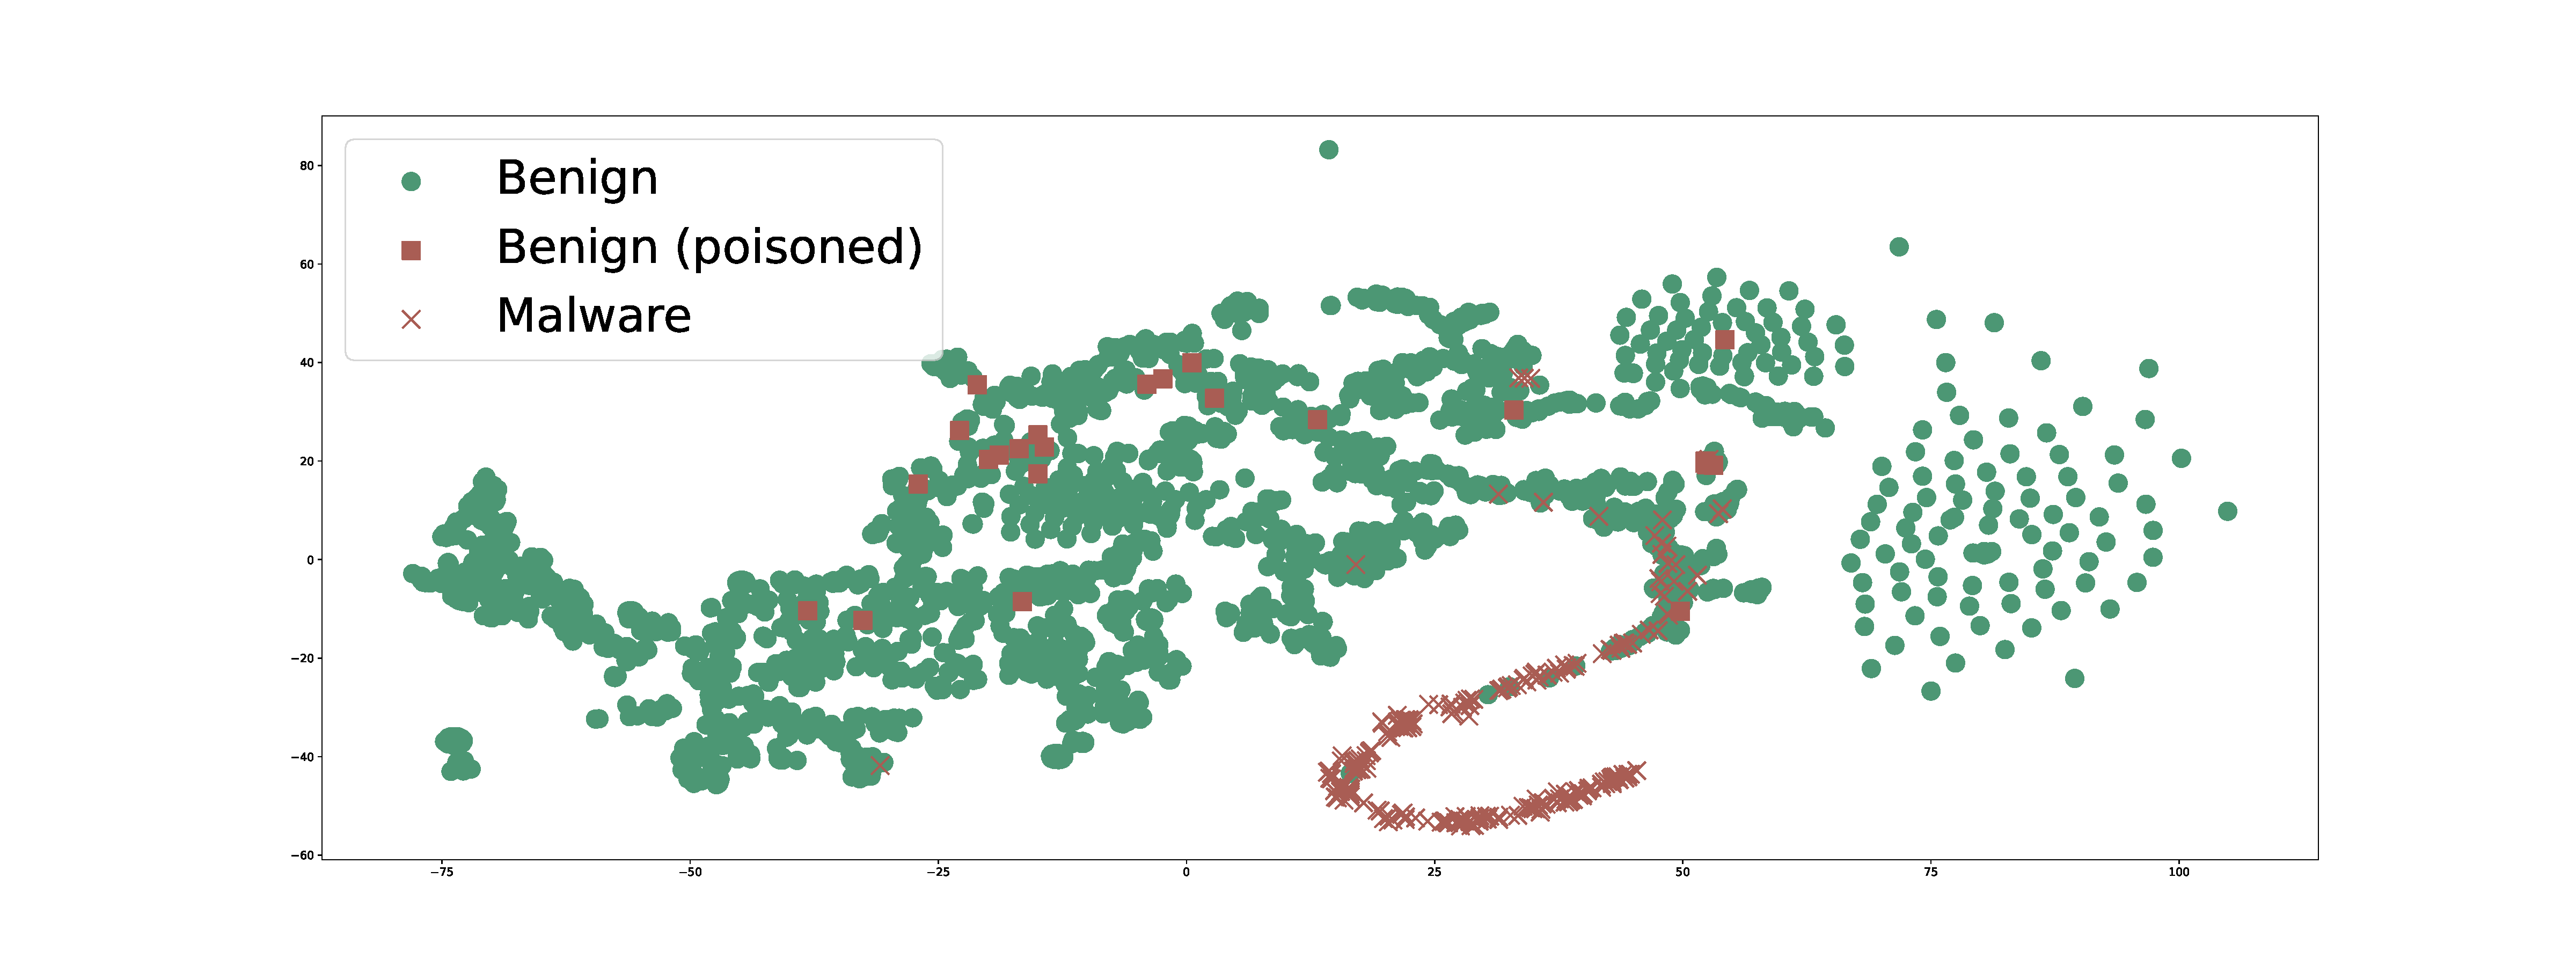
\includegraphics[width=\linewidth,keepaspectratio]{Graph/Evaluation/Figure24-v1}
%	\caption{Feature space entanglement}
%	\label{fig:feature space entanglement}
%\end{figure}
%Due to the longer time span of multi-target attack testing, we selected the APIGraph dataset for defense parameter analysis. 
%The number of clusters was the only parameter requiring manual configuration during the defense.
%We evaluated four cluster settings (6, 10, 20, and 40) under the multi-target attack. 
%The mean F1 score across these four settings was 0.91, with a variance of 0.0025.
%In the single-target attack, we selected the family 'clicks' (with the best ICDF defense performance) and the family 'mogap' (with the worst ICDF defense performance) from the Top 10 attack targets.
%For each family, we conducted four experiments with clustering parameter settings of 6, 10, 20, and 40 and observed that the defense performance remained consistent across all settings.
%This indicates that the defense parameter settings have minimal impact on defense effectiveness, which can effectively reduce the deployment costs of the defense method.

%\section{Practical Significance of \pandora}
%\label{Sec: Practical Significance of \pandora Attacks}
%Attackers can degrade the performance of target models, posing significant threats to the safety of real-world users.
%These risks are particularly severe in sensitive domains such as malware detection and industrial risk analysis, where attacks can lead to financial and physical harm to users.
%In the malware detection scenario studied in this paper, \pandora (under TPA) extends the misclassification duration of specific targets (malware), resulting in longer survival times in real-world scenarios.
%This prolonged survival exacerbates security threats.
%For example, the GriftHorse malware~\cite{GriftHorseMalware}, discovered in November 2020, leveraged subscription-based SMS services to generate 1.5 million USD to 4 million USD in monthly revenue, infecting over 10 million Android devices across 70+ countries.
%If the attacker combines the \pandora attack simultaneously, the harm of the above-mentioned security incident may be further expanded.
%Furthermore, the successful attack targets of \pandora serve as valuable references for attackers in designing future malware, significantly enhancing the efficiency of malware development and amplifying its potential harm.

%\section{Case Study}
%To verify the practicality of leveraging inference uncertainty in real-world machine learning models, we also tested publicly available machine learning services, specifically Baidu's object recognition system~\cite{Baidu-ImageRecognition}. 
%Ten categories from the CIFAR-10 dataset were selected for evaluation.
%Image recognition models show lower uncertainty with single-concept images but higher uncertainty with multi-concept images.
%To explore this, we created conceptual combinations using GAI technologies, enabling attackers to manipulate sample uncertainty in mature machine-learning products.
%The images were generated by progressively increasing the number of conceptual elements, ranging from 1 to 10, with subsequent images incorporating more concepts.
%For detailed information about the images, please refer to Appendix~\ref{Sec: Uncertainty Dynamics based on LLM}.
%\begin{figure}[htbp]
%	\centering
%	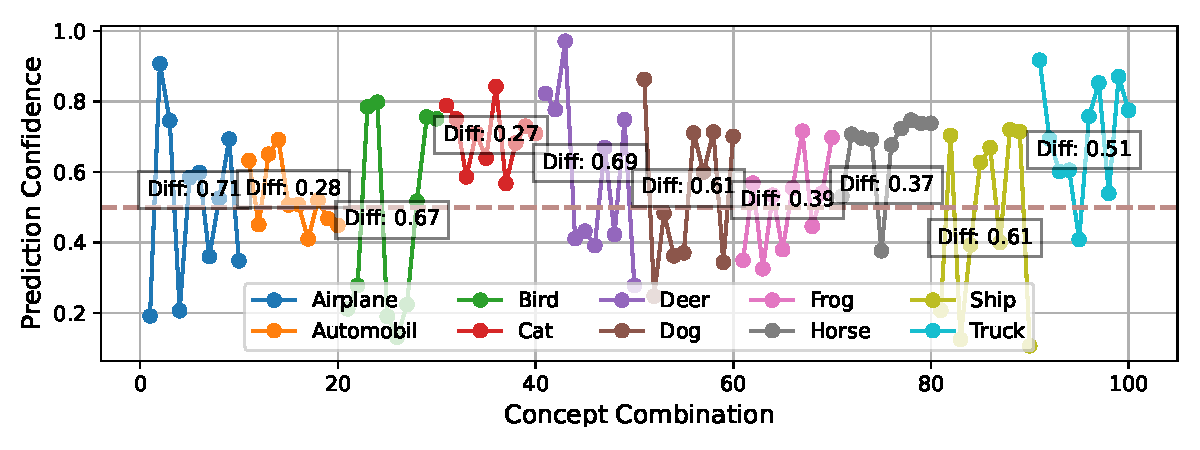
\includegraphics[width=\linewidth,keepaspectratio]{Graph/Evaluation/Figure18.pdf}
%	\caption{Case Study of Uncertainty Dynamics}
%	\label{fig:Case Study of Uncertainty Dynamics}
%\end{figure}
%Figure~\ref{fig:Case Study of Uncertainty Dynamics} illustrates notable fluctuations in sample uncertainty as additional concepts are introduced, with an average range of 0.511 between the highest and lowest uncertainty scores.
%Specifically, 90\% of test categories display uncertainty scores above 0.5 during conceptual combination tests, underscoring the vulnerability of mature machine learning models to manipulations in uncertainty.

%\subsection{Open Science}
%\label{Sec: Open Science}
%\noindent In order to enhance the reproducibility and replicability of scientific findings, we will share our research artifacts. 
%Our code (\url{}) and CDAMAL dataset (\url{https://anonymous.4open.science/r/CDAMAL-Concept-Drift-Dataset-3E08}) are all available. 
%In addition, considering research ethics, our dataset and the source code of the \pandora attack will only share minimized demonstration examples by default to illustrate the attack's effectiveness.
	
\end{document}
\endinput